%% LyX 2.3.4.2 created this file.  For more info, see http://www.lyx.org/.
%% Do not edit unless you really know what you are doing.
\documentclass{book}
\usepackage[T1]{fontenc}
\usepackage[utf8]{inputenc}
\setcounter{secnumdepth}{3}
\usepackage{array}
\usepackage{prettyref}
\usepackage{float}
\usepackage{units}
\usepackage{mathtools}
\usepackage{multirow}
\usepackage{amsmath}
\usepackage{amsthm}
\usepackage{amssymb}
\usepackage{stackrel}
\usepackage{graphicx}
\usepackage{setspace}
\onehalfspacing

\makeatletter

%%%%%%%%%%%%%%%%%%%%%%%%%%%%%% LyX specific LaTeX commands.
%% Because html converters don't know tabularnewline
\providecommand{\tabularnewline}{\\}

%%%%%%%%%%%%%%%%%%%%%%%%%%%%%% Textclass specific LaTeX commands.
\theoremstyle{plain}
\ifx\thechapter\undefined
	\newtheorem{thm}{\protect\theoremname}
\else
	\newtheorem{thm}{\protect\theoremname}[chapter]
\fi
\theoremstyle{definition}
\newtheorem{defn}[thm]{\protect\definitionname}
\theoremstyle{plain}
\newtheorem{lem}[thm]{\protect\lemmaname}
\theoremstyle{remark}
\newtheorem{note}[thm]{\protect\notename}
\theoremstyle{definition}
\newtheorem{example}[thm]{\protect\examplename}

%%%%%%%%%%%%%%%%%%%%%%%%%%%%%% User specified LaTeX commands.
\usepackage{Style_book}

\usepackage{color}
\usepackage{graphicx}
\graphicspath{{Images/}}

\expandafter\def\expandafter\normalsize\expandafter{%
    \normalsize
    \setlength\abovedisplayskip{4pt}
    \setlength\belowdisplayskip{4pt}
    \setlength\abovedisplayshortskip{4pt}
    \setlength\belowdisplayshortskip{4pt}
}

\renewcommand*\arraystretch{1.5}

\makeatother

\providecommand{\definitionname}{Definice}
\providecommand{\examplename}{Příklad}
\providecommand{\lemmaname}{Lemma}
\providecommand{\notename}{Poznámka}
\providecommand{\theoremname}{Věta}

\begin{document}
\thispagestyle{empty}
\frontmatter
\begin{center}
\begin{minipage}[c][0.2\textheight][t]{0.2\linewidth}%
\noindent \begin{center}

\includegraphics[width=3cm]{Images/Logos/Logo_cvut_col}
\par\end{center}%
\end{minipage}%
\begin{minipage}[c][0.2\textheight]{0.6\linewidth}%
\begin{center}
\color{doc_col}\textbf{\textsc{\Large{}České vysoké učení technické
v Praze}}{\Large\par}
\par\end{center}
\begin{center}
\color{doc_col}{\Large{}Fakulta jaderná a fyzikálně inženýrská}{\Large\par}
\par\end{center}
\begin{center}
\color{doc_col}{\Large{}Katedra matematiky}{\Large\par}
\par\end{center}%
\end{minipage}%
\begin{minipage}[c][0.2\textheight][t]{0.2\linewidth}%
\noindent \begin{center}

\includegraphics[width=3cm]{Images/Logos/Logo_fjfi_col}
\par\end{center}%
\end{minipage}
\par\end{center}

\begin{center}
\vspace{5cm}
\par\end{center}

\begin{center}
\textbf{\huge{}Rozpoznávání a zpracování obrazu}{\huge\par}
\par\end{center}

\begin{center}
{\huge{}\vspace{3cm}
}{\huge\par}
\par\end{center}

\begin{center}
\emph{\large{}Poznámky k přednáškám (vytvořeno: 2. 1. 2018)}\vfill{}
\par\end{center}

\tableofcontents{}

\cleardoublepage{}

\chapter*{Úvodní slovo}

\addcontentsline{toc}{chapter}{Úvodní slovo}
\markboth{Úvodní slovo}{}

Tyto poznámky vznikly jako materiál ke státní závěrečné zkoušce z
předmětů ROZ1, ROZ2 a SFTO v roce 2017. Vzhledem k tomu, že se jedná
o studenty vytvořené poznámky, tak není možné zaručit jejich bezchybnost.
Berte proto tyto poznámky pouze jako pomocný materiál a nespoléhejte
při učení pouze na ně. 

\subsubsection*{Oprava chyb}

Jak již bylo zmíněno výše, poznámky jsou studentské a tedy obsahují
chyby. Například část \textcolor{doc_col}{\textbf{\emph{Příznakové
metody (signálově nezávislé)}}} je velmi nepřesná a potřebovala by
předělat.

\subsubsection*{Verze dokumentu: }
\begin{itemize}
\item Martin Petřek (původní verze),
\item Ondřej Ticháček (první přepracování),
\item Václav Mácha, Jana Vacková (současná verze).
\end{itemize}
\cleardoublepage{}

\mainmatter

\chapter{Matematické základy}

\section{Konvoluce a korelace}
\begin{defn}[Konvoluce a korelace v 1D]
 Konvolucí rozumíme zobrazení $\ast:L_{1}\times L_{1}\rightarrow L_{1}$
definované pro funkce $f,g$ vztahem 
\begin{align*}
(f\ast g)(x) & =\int\limits _{\mathbb{R}}f(t)g(x-t)\textrm{d}t, &  & \textrm{pro spojitý případ,}\\
(f\ast g)(n) & =\stackrel[m=-\infty]{\infty}{\sum}f\left(m\right)g\left(n-m\right), &  & \textrm{pro diskrétní případ.}
\end{align*}
 Korelací rozumíme zobrazení $\circledast:L_{1}\times L_{1}\rightarrow L_{1}$
definované pro funkce $f,g$ vztahem 
\begin{align*}
\left(f\circledast g\right)\left(x\right) & =\int\limits _{\mathbb{R}}f(t)g\left(t-x\right)\textrm{d}t, &  & \textrm{pro spojitý případ,}\\
\left(f\circledast g\right)\left(n\right) & =\stackrel[m=-\infty]{\infty}{\sum}f\left(m\right)g\left(m-n\right), &  & \textrm{pro diskrétní případ.}
\end{align*}
\end{defn}

Princip konvoluce je znázorněn na obr. \ref{fig:Konvoluce_1D}. V
podstatě se jedná o průměrování funkce $f$ jinou funkcí $g$, protože
$g$ je většinou symetrická funkce s malým nosičem. Je-li např. $g$
obdélníkový puls, pak se jedná o klasické průměrování. Dost často
se požaduje, aby výsledná funkce $f\ast g$ měla stejně omezený obor
hodnot jako původní funkce $f$, z tohoto důvodu se volí $g$ splňující
vlastnost $\int_{\mathbb{R}}g=1$. Rozdíl korelace oproti konvoluci
je, že funkce $g$ se v korelaci ,,neotáčí``.
\begin{figure}[h]
\centering{}%% Creator: Inkscape 0.91, www.inkscape.org
%% PDF/EPS/PS + LaTeX output extension by Johan Engelen, 2010
%% Accompanies image file 'Konvoluce_1D.pdf' (pdf, eps, ps)
%%
%% To include the image in your LaTeX document, write
%%   \input{<filename>.pdf_tex}
%%  instead of
%%   \includegraphics{<filename>.pdf}
%% To scale the image, write
%%   \def\svgwidth{<desired width>}
%%   \input{<filename>.pdf_tex}
%%  instead of
%%   \includegraphics[width=<desired width>]{<filename>.pdf}
%%
%% Images with a different path to the parent latex file can
%% be accessed with the `import' package (which may need to be
%% installed) using
%%   \usepackage{import}
%% in the preamble, and then including the image with
%%   \import{<path to file>}{<filename>.pdf_tex}
%% Alternatively, one can specify
%%   \graphicspath{{<path to file>/}}
%%
%% For more information, please see info/svg-inkscape on CTAN:
%%   http://tug.ctan.org/tex-archive/info/svg-inkscape
%%
\begingroup%
  \makeatletter%
  \providecommand\color[2][]{%
    \errmessage{(Inkscape) Color is used for the text in Inkscape, but the package 'color.sty' is not loaded}%
    \renewcommand\color[2][]{}%
  }%
  \providecommand\transparent[1]{%
    \errmessage{(Inkscape) Transparency is used (non-zero) for the text in Inkscape, but the package 'transparent.sty' is not loaded}%
    \renewcommand\transparent[1]{}%
  }%
  \providecommand\rotatebox[2]{#2}%
  \ifx\svgwidth\undefined%
    \setlength{\unitlength}{264bp}%
    \ifx\svgscale\undefined%
      \relax%
    \else%
      \setlength{\unitlength}{\unitlength * \real{\svgscale}}%
    \fi%
  \else%
    \setlength{\unitlength}{\svgwidth}%
  \fi%
  \global\let\svgwidth\undefined%
  \global\let\svgscale\undefined%
  \makeatother%
  \begin{picture}(1,0.40909091)%
    \put(0.18181818,0.10606087){\color[rgb]{0,0,0}\makebox(0,0)[lb]{\smash{\footnotesize $g(x)$}}}%
    \put(0.10644587,0.22727281){\color[rgb]{0,0,0}\makebox(0,0)[b]{\smash{\footnotesize $f(x)$}}}%
    \put(0,0){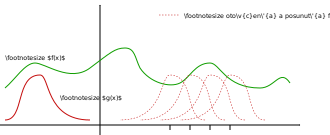
\includegraphics[width=\unitlength,page=1]{Konvoluce_1D.pdf}}%
    \put(0.55757576,0.35454553){\color[rgb]{0,0,0}\makebox(0,0)[lb]{\smash{\footnotesize oto\v{c}en\'{a} a posunut\'{a} funkce $g(x)$}}}%
  \end{picture}%
\endgroup%
\caption{Znázornění principu konvoluce v 1D.\label{fig:Konvoluce_1D}}
\end{figure}

\begin{defn}[Diracova $\delta$ funkce]
 Diracovou $\delta$ funkcí rozumíme funkci $\text{\ensuremath{\delta}}\left(x\right)$
splňující
\[
\text{\ensuremath{\delta}}\left(x\right)=\left\{ \begin{array}{ccc}
"+\infty" & \ldots & x=0\\
0 & \ldots & x\neq0
\end{array}\right.,\quad\wedge\quad\int\limits _{\mathbb{R}}\delta\left(x\right)\textrm{d}x=1.
\]
\end{defn}

\begin{lem}
Základní vlastnosti konvoluce:
\begin{align*}
\textnormal{1.}\; & f\left(x\right)\ast g\left(x\right)=g\left(x\right)\ast f\left(x\right), & \textnormal{4.}\; & a\left(f\left(x\right)\ast g\left(x\right)\right)=\left(af\left(x\right)\right)\ast g\left(x\right)=f\left(x\right)\ast\left(ag\left(x\right)\right),\\
\textnormal{2.}\; & f\left(x\right)\ast\left(g\left(x\right)+h\left(x\right)\right)=f\left(x\right)\ast g\left(x\right)+f\left(x\right)\ast h\left(x\right), & \textnormal{5.}\; & f\left(x\right)\ast\delta\left(x\right)=\delta\left(x\right)\ast f\left(x\right)=f\left(x\right).\\
\textnormal{3.}\; & f\left(x\right)\ast\left(g\left(x\right)\ast h\left(x\right)\right)=\left(f\left(x\right)\ast g\left(x\right)\right)\ast h\left(x\right),
\end{align*}
\end{lem}

\begin{defn}[Konvoluce a korelace v 2D]
 Konvoluce a korelace ve 2D jsou pro matice $F$, $G$ definovány
po prvcích následovně
\begin{align*}
H\left[i,j\right] & =\stackrel[u=-k]{k}{\sum}\:\stackrel[v=-k]{k}{\sum}G\left[u,v\right]F\left[i-u,j-v\right],\\
H\left[i,j\right] & =\stackrel[u=-k]{k}{\sum}\:\stackrel[v=-k]{k}{\sum}G\left[u,v\right]F\left[i+u,j+v\right].
\end{align*}
\end{defn}

V případě konvoluce se jedná o posouvání matice $G$, kterou nazýváme
maska, po matici $F$ a do každého bodu výsledné matice napíšeme součet
součinů překrývajících se prvků. V případě korelace se maska aplikuje
obráceně. Koeficienty v masce udávají váhu jednotlivým pixelům. Aby
při aplikaci masky na obrázek nedocházelo ke zvyšování jasu, je třeba,
aby celková energie masky byla 1.

Při aplikaci masky na obrázek dochází na okrajích k tzv. okrajovému
efektu. Na obr. \ref{fig:Okrajovy_efekt} jsou znázorněny možnosti
aplikace masky. Ve většině případů chceme, aby výsledný obrázek byl
stejně velký jako původní obrázek $F$, proto volíme typ \emph{same}.
V takovém případě je ovšem nutné původní obrázek rozšířit. Toto rozšíření
lze dělat několika způsoby:
\begin{itemize}
\item \textbf{přidání nul (}\textbf{\emph{zero padding}}\textbf{):} po aplikaci
masky dojde k rozmazání a ztmavnutí okrajů a vzniká hrana,
\item \textbf{zrcadlení (}\textbf{\emph{mirror extension}}\textbf{): }nedochází
ke ztmavnutí ani rozmazání a nevzniká hrana,
\item \textbf{periodické prodloužení (}\textbf{\emph{periodic extension}}\textbf{):
}toto vyžadují některé matematické věty (např. konvoluce).
\end{itemize}
\begin{figure}[h]
\centering{}%% Creator: Inkscape 0.91, www.inkscape.org
%% PDF/EPS/PS + LaTeX output extension by Johan Engelen, 2010
%% Accompanies image file 'Okrajovy_efekt.pdf' (pdf, eps, ps)
%%
%% To include the image in your LaTeX document, write
%%   \input{<filename>.pdf_tex}
%%  instead of
%%   \includegraphics{<filename>.pdf}
%% To scale the image, write
%%   \def\svgwidth{<desired width>}
%%   \input{<filename>.pdf_tex}
%%  instead of
%%   \includegraphics[width=<desired width>]{<filename>.pdf}
%%
%% Images with a different path to the parent latex file can
%% be accessed with the `import' package (which may need to be
%% installed) using
%%   \usepackage{import}
%% in the preamble, and then including the image with
%%   \import{<path to file>}{<filename>.pdf_tex}
%% Alternatively, one can specify
%%   \graphicspath{{<path to file>/}}
%%
%% For more information, please see info/svg-inkscape on CTAN:
%%   http://tug.ctan.org/tex-archive/info/svg-inkscape
%%
\begingroup%
  \makeatletter%
  \providecommand\color[2][]{%
    \errmessage{(Inkscape) Color is used for the text in Inkscape, but the package 'color.sty' is not loaded}%
    \renewcommand\color[2][]{}%
  }%
  \providecommand\transparent[1]{%
    \errmessage{(Inkscape) Transparency is used (non-zero) for the text in Inkscape, but the package 'transparent.sty' is not loaded}%
    \renewcommand\transparent[1]{}%
  }%
  \providecommand\rotatebox[2]{#2}%
  \ifx\svgwidth\undefined%
    \setlength{\unitlength}{268bp}%
    \ifx\svgscale\undefined%
      \relax%
    \else%
      \setlength{\unitlength}{\unitlength * \real{\svgscale}}%
    \fi%
  \else%
    \setlength{\unitlength}{\svgwidth}%
  \fi%
  \global\let\svgwidth\undefined%
  \global\let\svgscale\undefined%
  \makeatother%
  \begin{picture}(1,0.40298507)%
    \put(0.18054268,0.20256373){\color[rgb]{0,0,0}\makebox(0,0)[lb]{\smash{}}}%
    \put(1.24916156,0.62585506){\color[rgb]{0,0,0}\makebox(0,0)[lb]{\smash{}}}%
    \put(0.82646509,0.1360722){\color[rgb]{0,0,0}\makebox(0,0)[lb]{\smash{}}}%
    \put(0.49222445,0.26964933){\color[rgb]{0,0,0}\makebox(0,0)[lb]{\smash{}}}%
    \put(0,0){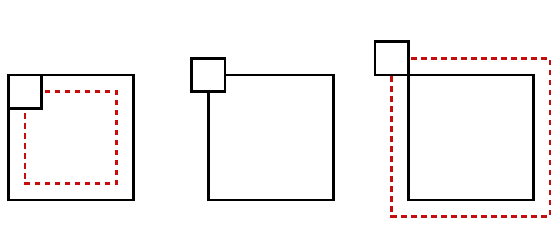
\includegraphics[width=\unitlength,page=1]{Okrajovy_efekt.pdf}}%
    \put(0.04477608,0.2238806){\color[rgb]{0,0,0}\makebox(0,0)[b]{\smash{G}}}%
    \put(0.1253731,0.14925373){\color[rgb]{0,0,0}\makebox(0,0)[b]{\smash{F}}}%
    \put(0.48358234,0.14925373){\color[rgb]{0,0,0}\makebox(0,0)[b]{\smash{F}}}%
    \put(0.84179135,0.14925373){\color[rgb]{0,0,0}\makebox(0,0)[b]{\smash{F}}}%
    \put(0.84179135,0.37313436){\color[rgb]{0,0,0}\makebox(0,0)[b]{\smash{\textbf C)}}}%
    \put(0.48358126,0.37313436){\color[rgb]{0,0,0}\makebox(0,0)[b]{\smash{\textbf B)}}}%
    \put(0.12537226,0.37313436){\color[rgb]{0,0,0}\makebox(0,0)[b]{\smash{\textbf A)}}}%
    \put(0.70149299,0.28358061){\color[rgb]{0,0,0}\makebox(0,0)[b]{\smash{G}}}%
    \put(0.37313473,0.25372986){\color[rgb]{0,0,0}\makebox(0,0)[b]{\smash{G}}}%
  \end{picture}%
\endgroup%
\caption{Ukázka okrajového efektu při diskrétní konvoluci ve 2D. Typy: \textbf{A)}
\emph{valid}, \textbf{B)} \emph{same} a \textbf{C)} \emph{full}. \label{fig:Okrajovy_efekt}}
\end{figure}


\section{Fourierova transformace}

Fourierova řada slouží k zápisu periodického průběhu pomocí funkcí
$\sin$ a $\cos$. Základní myšlenka zápisu funkce ve formě řady z
těchto funkcí je rozklad vektoru do ortogonální báze. Mějme ortogonální
bázi $\mathcal{B}=\left\{ \phi_{n}\left(x\right)\right\} =\{1,\sin mx,\cos nx\}$
v diskrétním prostoru $L_{2}\left(\left\langle 0,2\pi\right\rangle \right)$
se skalárním součinem definovaným následovně
\[
\left\langle f,g\right\rangle =\int\limits _{0}^{2\pi}f\left(x\right)g\left(x\right)\textrm{d}x.
\]
Funkci $f\in L_{2}\left(\left\langle 0,2\pi\right\rangle \right)$
jsme pak schopni vyjádřit pomocí Fourierovy řady
\[
f=\frac{a_{0}}{2}+\stackrel[k=1]{+\infty}{\sum}\left[a_{k}\cos\left(kx\right)+b_{k}\sin\left(kx\right)\right],
\]
\begin{align*}
a_{0} & =\frac{1}{\pi}\int\limits _{0}^{2\pi}f\left(x\right)\textrm{d}x, & a_{k} & =\frac{1}{\pi}\int\limits _{0}^{2\pi}f\left(x\right)\cos\left(kx\right)\textrm{d}x\quad k\geq1, & b_{k} & =\frac{1}{\pi}\int\limits _{0}^{2\pi}f\left(x\right)\sin\left(kx\right)\textrm{d}x,\quad k\geq1,
\end{align*}
kde $a_{k}$ a $b_{k}$ jsou tzv. Fourierovy koeficienty. To, že jsme
se omezili pouze na celočíselné násobky frekvencí, má za následek
fakt, že jsme schopni v celém oboru popsat jen periodické funkce.
V obecném pojetí lze libovolnou funkci složit z bazických $\sin$
a $\cos$ funkcí, ovšem jejich frekvence musí být spojitě se měnící. 

Fourierova transformace je integrální transformace převádějící signál
mezi časově a frekvenčně závislým vyjádřením pomocí harmonických signálů.
V podstatě se jedná o vyjádření původní funkce jako lineární kombinace
$\sin$ a $\cos$ funkcí. Slouží pro převod signálů z časové oblasti
do oblasti frekvenční. V jednodimenzionálním případě jsou bázové funkce
ve tvaru 
\[
\left\{ \phi_{u}\left(x\right)\right\} =\left\{ e^{-2\pi iux}\right\} 
\]
 a ve dvoudimenzionálním případě jsou bázové funkce ve tvaru 
\[
\left\{ \phi_{uv}\left(x,y\right)\right\} =\left\{ e^{-2\pi i\left(ux+vy\right)}\right\} 
\]
 a jejich reálná a imaginární část je tvořena ,,vlnitými plechy``.
\begin{defn}[Spojitá Fourierova transformace (CFT) a inverzní spojitá Fourierova
transformace (IFT)]
 Nechť $f\in L_{1}$, pak spojitá Fourierova transformace je definována
vztahem
\begin{align*}
F\left(u\right) & =\mathcal{F}\left[f(x)\right]\left(u\right)=\int\limits _{\mathbb{R}}f\left(x\right)e^{-2\pi iux}\textrm{d}x & \textrm{v 1D},\\
F\left(u,v\right) & =\mathcal{F}\left[f\left(x,y\right)\right]\left(u,v\right)=\int\limits _{\mathbb{R}^{2}}f\left(x,y\right)e^{-2\pi i\left(ux+vy\right)}\textrm{d}x\textrm{d}y & \textrm{ve 2D}.
\end{align*}
Inverzní Fourierovu transformaci definujeme následovně
\begin{align*}
f\left(x\right) & =\mathcal{F}^{-1}\left[F\left(u\right)\right]\left(x\right)=\int\limits _{\mathbb{R}}F\left(u\right)e^{2\pi iux}\textrm{d}u & \textrm{v 1D},\\
f\left(x,y\right) & =\mathcal{F}^{-1}\left[F\left(u,v\right)\right]\left(x,y\right)=\int\limits _{\mathbb{R}^{2}}F\left(u,v\right)e^{2\pi i\left(ux+vy\right)}\textrm{d}u\textrm{d}v & \textrm{ve 2D}.
\end{align*}
\end{defn}

\begin{note}
Fourierova transformace a spojitá Fourierova transformace se nepatrně
liší
\begin{align*}
\mathcal{F}\left[f\left(x\right)\right] & =\int\limits _{\mathbb{R}}f\left(x\right)e^{-iux}\textrm{d}x, & \mathcal{F}^{-1}\left[F\left(u\right)\right] & =\frac{1}{2\pi}\int\limits _{\mathbb{R}}F\left(u\right)e^{iux}\textrm{d}u.
\end{align*}
\end{note}

\begin{defn}[Diskrétní Fourierova transformace]
 Diskrétní Fourierova transformace a inverzní diskrétní Fourierova
jsou definovány vztahy
\begin{align*}
F\left(k\right) & =\mathcal{F}\left[f(n)\right]\left(k\right)=\stackrel[n=0]{N-1}{\sum}f\left(n\right)e^{-\frac{1}{N}2\pi ink}, & \forall k & \in\left\{ 0,1,\ldots,N-1\right\} ,\\
f\left(n\right) & =\mathcal{F}^{-1}\left[F\left(k\right)\right]\left(n\right)=\frac{1}{N}\cdot\stackrel[k=0]{N-1}{\sum}F\left(k\right)e^{\frac{1}{N}2\pi ink}, & \forall n & \in\left\{ 0,1,\ldots,N-1\right\} .
\end{align*}
\end{defn}

Existence komplexní funkce $F$ plyne z předpokladu, není ovšem zaručeno,
že i $F\left(u\right)$ bude z $L_{1}$. Díky tomu, že $F\left(u\right)$
je komplexní funkce (spektrum), lze jí rozložit do tvaru
\[
F\left(u\right)=\left|F\left(u\right)\right|e^{i\arg F\left(u\right)},
\]
kde $\left|F\left(u\right)\right|$ je tzv. amplitudové spektrum a
$\arg F\left(u\right)$ fázové spektrum.
\begin{lem}
Vlastnosti Fourierovy transformace:
\begin{align*}
\textnormal{1.}\; & \mathcal{F}\left[af\left(x\right)+g\left(x\right)\right]\left(u\right)=a\mathcal{F}\left[f\left(x\right)\right]\left(u\right)+\mathcal{F}\left[g\left(x\right)\right]\left(u\right), & \textnormal{4.}\; & \mathcal{F}\left[1\right]\left(u\right)=\delta\left(u\right),\\
\textnormal{2.}\; & \mathcal{F}\left[a\cdot f\left(x\right)\right]\left(u\right)=\left|a\right|^{-1}\mathcal{F}\left[f\left(x\right)\right]\left(\frac{u}{a}\right), & \textnormal{5.}\; & \mathcal{F}\left[R\left(f\left(x\right)\right)\right]\left(u\right)=R\left(\mathcal{F}\left[f\left(x\right)\right]\left(u\right)\right),\\
\textnormal{3.}\; & \mathcal{F}\left[\delta\left(x\right)\right]=1,
\end{align*}
kde $R\left(.\right)$ značí rotaci.
\end{lem}

\begin{thm}[Fourier Shift teorém ]
 \label{thm:Fourier_Shift_Theorem}Posuneme-li funkci $f$ o konstantu
$a$, dává Fourierova transformace vztah:
\[
\mathcal{F}\left[f(x-a)\right]\left(u\right)=e^{-2\pi iau}F(u).
\]
\end{thm}

\begin{proof}
Upravujme
\begin{align*}
\mathcal{F}\left[f\left(x-a\right)\right]\left(u\right) & =\int\limits _{\mathbb{R}}f\left(x-a\right)e^{-2\pi iu(x\pm a)}\textrm{d}x=e^{-2\pi iua}\int\limits _{\mathbb{R}}f\left(x-a\right)e^{-2\pi iu(x-a)}\textrm{d}x=\left|\begin{array}{c}
y=x-a\\
\textrm{d}y=\textrm{d}x
\end{array}\right|=\\
 & =e^{-2\pi iua}\int\limits _{\mathbb{R}}f\left(y\right)e^{-2\pi iuy}\textrm{d}y=e^{-2\pi iua}F\left(u\right).
\end{align*}
\end{proof}
Tedy obraz je akorát násobený komplexní jednotkou $e^{-2\pi iau}$,
tj. jeho amplituda má stejnou velikost jako originál. Toho lze využít
pro rozpoznávání, fázi lze zjistit dodatečně. Lze také ukázat, že
nejpodstatnější část obrazové informace je obsažena ve fázi, amplituda
nemá tak zásadní vliv na vzhled obrazu.
\begin{thm}[Konvoluční teorém]
Pro Fourierovu transformaci platí následující vztahy
\begin{align*}
\mathcal{F}\left[f\left(x\right)\ast g\left(x\right)\right]\left(u\right) & =F\left(u\right)\cdot G\left(u\right),\\
\mathcal{F}\left[f\left(x\right)\cdot g\left(x\right)\right]\left(u\right) & =F\left(u\right)\ast G\left(u\right),
\end{align*}
kde symbol $\cdot$ značí násobení stejně rozměrných matic po prvcích.
\end{thm}

\begin{proof}
Upravujme
\begin{align*}
\mathcal{F}\left[f\left(x\right)\ast g\left(x\right)\right]\left(u\right) & =\int\limits _{\mathbb{R}}\left[\int\limits _{\mathbb{R}}f(t)g(x-t)\textrm{d}t\right]e^{-2\pi iux}\textrm{d}x\overset{a)}{=}\int\limits _{\mathbb{R}}f(t)\left[\int\limits _{\mathbb{R}}g(x-t)e^{-2\pi iux}\textrm{d}x\right]\textrm{d}t=\\
 & \overset{b)}{=}\int\limits _{\mathbb{R}}f(t)\left[e^{-2\pi itu}G(u)\right]\textrm{d}t=\int\limits _{\mathbb{R}}f(t)e^{-2\pi itu}\textrm{d}t\cdot G(u)=F(u)\cdot G(u),
\end{align*}
kde jsme v rovnosti $a)$ použili Fubiniho větu a v rovnosti $b)$
větu \ref{thm:Fourier_Shift_Theorem}. Druhou rovnost dokážeme obdobně
\begin{align*}
\mathcal{F}\left[f\left(x\right)\cdot g\left(x\right)\right]\left(u\right) & =\int\limits _{\mathbb{R}}f\left(x\right)g\left(x\right)e^{-2\pi iux}\textrm{d}x\overset{a)}{=}\int\limits _{\mathbb{R}}\left[\int\limits _{\mathbb{R}}F\left(t\right)e^{2\pi itx}\textrm{d}t\right]g\left(x\right)e^{-2\pi iux}\textrm{d}x=\\
 & \overset{c)}{=}\int\limits _{\mathbb{R}}F\left(t\right)\left[\int\limits _{\mathbb{R}}g\left(x\right)e^{-2\pi i\left(u-t\right)x}\textrm{d}x\right]\textrm{d}t=\int\limits _{\mathbb{R}}F\left(t\right)G\left(u-t\right)\textrm{d}t=F(u)\ast G(u),
\end{align*}
kde jsme v rovnosti $a)$ použili inverzní Fourierovu transformaci
a v rovnosti $b)$ Fubiniho větu.
\end{proof}
Pokud chceme ověřit konvoluční teorém v praxi, je potřeba diskrétní
data periodicky prodlužovat! Co se týká náročnosti, má výpočet diskrétní
Fourierovy transformace v základním tvaru složitost $O\left(N^{2}\right)$.
V roce 1942 pánové Danielson a Lanczos zjistili, že posloupnosti délky
$N=2^{k}$ lze vyjádřit jako součet dvou diskrétních Fourierových
transformací délky $\frac{N}{2},$ kde v jedné jsou liché a ve druhé
sudé vzorky. V roce 1965 Cooley a Turkey zobecnili tuto metodu i pro
posloupnosti délky $N\neq2^{k}$. Tato rychlá Fourierova transformace
(FFT) se používá dodnes. Lze ji sestrojit pro obecné obdélníkové matice
a její složitost je $O\left(N\cdot\log_{2}N\right)$. Naproti tomu
konvoluce má složitost $O\left(N^{2}\right)$ pro každý bod masky,
tedy je jasné, že při počítání konvoluce s rozměrnějšími maticemi
je výhodnější použít konvolučního teorému a ve frekvenční oblasti
pouze vynásobit matice.
\begin{example}[Funkce $\textrm{sinc\ensuremath{\left(x\right)}}$]
Nyní ukažme jak vypadá Fourierův obraz \emph{obdélníkového pulsu}.
Nechť $f$ je funkce definovaná pro $c\in\mathbb{R}$ a $\lambda\in\mathbb{R}^{+}$
jako 
\begin{align*}
f(x) & =\left\{ \begin{array}{ccc}
c & \ldots & x\in\langle-\lambda,\lambda\rangle,\\
0 & \ldots & \text{jinde},
\end{array}\right.
\end{align*}
pak
\[
F(u)=\int\limits _{\mathbb{R}}f(x)e^{-2\pi iux}\textrm{d}x=c\int\limits _{-\lambda}^{\lambda}e^{-2\pi iux}\textrm{d}x=\frac{c}{-2\pi iu}\left[e^{-2\pi uix}\right]_{-\lambda}^{\lambda}=c\frac{e^{-2\pi iu\lambda}-e^{2\pi iu\lambda}}{-2\pi iu}=\frac{c}{\pi u}\sin(2\pi\lambda u).
\]
Pro $c=1$ a $\lambda=\frac{1}{2}$ dostaneme funkci $\textnormal{sinc}$
\begin{align*}
F(u) & =\frac{\sin(\pi u)}{\pi u}=\textnormal{sinc}(u).
\end{align*}
Ve 2D vzniká funkce $\mathrm{sinc}\left(x,y\right)$, která je ve
tvaru
\[
\textnormal{sinc}\left(x,y\right)=\textnormal{sinc}(x)\textnormal{sinc}(y)=\frac{\sin\left(\pi x\right)\sin\left(\pi y\right)}{\pi^{2}xy}.
\]
\begin{figure}[H]
\centering{}\include{Images/Funkce_sinc}\caption{Fourierova transformace obdélníkového pulsu a vzniklá funkce $\textnormal{sinc}(x)$.}
\end{figure}
Tato funkce není středově symetrická, jak by se mohlo zdát. Další
velice zajímavou vlastnost obdélníkového pulsu získáme, pokud budeme
provádět konvoluci těchto pulsů. Opakováním konvoluce obdélníkových
pulsů totiž vznikají tzv. B-spline křivky, které stále lépe aproximují
Gaussovu funkci, viz obr. \ref{fig:B_spline}.
\begin{figure}[H]
\centering{}\include{Images/B-spline}\caption{Ukázka opakované konvoluce obdélníkových pulsů a vznik B-spline křivek.
\label{fig:B_spline}}
\end{figure}
\end{example}

Další důležitý signál je ve 2D obdélníkový signál, kruhový signál
a gaussovký signál. Amplitudové spektrum obdélníkového signálu je
tvořeno ,,protáhlou`` funkcí $\textnormal{sinc}$. Amplitudové spektrum
kruhového signálu je tvořeno Besselovou funkcí a spektrum gaussovského
signálu je opět Gaussova funkce. Tyto signály a jejich amplitudová
spektra jsou na obr. \ref{fig:FT_2D_signaly} a na obr. \ref{fig:FT_2D_signaly_ve_3D}
jsou jejich 3D znázornění.
\begin{figure}[h]
\begin{centering}
\begin{tabular}{ccccc}
\includegraphics[width=0.15\linewidth]{Images/PNG/FT_vzor7} &  & \includegraphics[width=0.15\linewidth]{Images/PNG/FT_vzor8} &  & \includegraphics[width=0.15\linewidth]{Images/PNG/FT_vzor9}\tabularnewline
$\Downarrow\mathcal{F}$ &  & $\Downarrow\mathcal{F}$ &  & $\Downarrow\mathcal{F}$\tabularnewline
\includegraphics[width=0.15\linewidth]{Images/PNG/FT_obraz7} &  & \includegraphics[width=0.15\linewidth]{Images/PNG/FT_obraz8} &  & \includegraphics[width=0.15\linewidth]{Images/PNG/FT_obraz9}\tabularnewline
\end{tabular}\caption{Ukázka dalších důležitých signálů a jejich amplitudové spektrum. \label{fig:FT_2D_signaly}}
\par\end{centering}
\end{figure}
\begin{figure}[p]
\centering{}%
\begin{tabular}{ccc}
\includegraphics[width=0.3\linewidth,height=0.13\textheight]{Images/PNG/FT_vzor_3D1} & \includegraphics[width=0.3\linewidth,height=0.13\textheight]{Images/PNG/FT_vzor_3D2} & \includegraphics[width=0.3\linewidth,height=0.13\textheight]{Images/PNG/FT_vzor_3D3}\tabularnewline
$\Downarrow\mathcal{F}$ & $\Downarrow\mathcal{F}$ & $\Downarrow\mathcal{F}$\tabularnewline
\includegraphics[width=0.3\linewidth,height=0.13\textheight]{Images/PNG/FT_obraz_3D1} & \includegraphics[width=0.3\linewidth,height=0.13\textheight]{Images/PNG/FT_obraz_3D2} & \includegraphics[width=0.3\linewidth,height=0.13\textheight]{Images/PNG/FT_obraz_3D3}\tabularnewline
\end{tabular}\caption{Reprezentace signálu z obr. \ref{fig:FT_2D_signaly} ve 3D, kde třetí
rozměr reprezentuje intenzitu v daném pixelu. \label{fig:FT_2D_signaly_ve_3D}}
\medskip{}
\begin{tabular}{cccccc}
\includegraphics[width=0.13\linewidth]{Images/PNG/FT_vzor1} & \includegraphics[width=0.13\linewidth]{Images/PNG/FT_vzor2} & \includegraphics[width=0.13\linewidth]{Images/PNG/FT_vzor3} & \includegraphics[width=0.13\linewidth]{Images/PNG/FT_vzor4} & \includegraphics[width=0.13\linewidth]{Images/PNG/FT_vzor5} & \includegraphics[width=0.13\linewidth]{Images/PNG/FT_vzor6}\tabularnewline
$\Downarrow\mathcal{F}$ & $\Downarrow\mathcal{F}$ & $\Downarrow\mathcal{F}$ & $\Downarrow\mathcal{F}$ & $\Downarrow\mathcal{F}$ & $\Downarrow\mathcal{F}$\tabularnewline
\includegraphics[width=0.13\linewidth]{Images/PNG/FT_obraz1} & \includegraphics[width=0.13\linewidth]{Images/PNG/FT_obraz2} & \includegraphics[width=0.13\linewidth]{Images/PNG/FT_obraz3} & \includegraphics[width=0.13\linewidth]{Images/PNG/FT_obraz4} & \includegraphics[width=0.13\linewidth]{Images/PNG/FT_obraz5} & \includegraphics[width=0.13\linewidth]{Images/PNG/FT_obraz6}\tabularnewline
\end{tabular}\caption{Ukázka amplitudového spektra vybraných pravidelných obrazů.\label{fig:FT_pravidelnosti}}
\medskip{}
\include{Images/Frekvencni_filtry}\caption{Filtry ve frekvenční oblasti: \textbf{A)} \emph{high-pass filtr},
\textbf{B)} \emph{low-pass filtr}, \textbf{C)} \emph{band-pass filtr},
\textbf{D)} \emph{Gaussovký high-pass filtr}, \textbf{E)} \emph{Gaussovký
low-pass filtr} a \textbf{F)} \emph{směrový filtr}. \label{fig:Filtry_frekvencni}}
\end{figure}


\subsection{Filtrace ve frekvenční oblasti}

Pokud provedeme Fourierovu transformaci 2D obrazu, získáme její projekci
do prostoru bazických funkcí a dozvíme se, jak jsou v obrazu zastoupeny
jednotlivé frekvence. Protože jsme ovšem původně měli reálný signál,
bude Fourierův obraz symetrický podle středu. V bodě $\left(0,0\right)$
se nachází celková energie (součet intenzit jednotlivých pixelů) Fourierova
obrazu, protože 
\[
F\left(0,0\right)=\stackrel[n=0]{N-1}{\sum}\stackrel[m=0]{M-1}{\sum}f\left(n,m\right)e^{-2\pi i\left(\frac{1}{N}n0+\frac{1}{M}m0\right)}=\stackrel[n=0]{N-1}{\sum}\stackrel[m=0]{M-1}{\sum}f\left(n,m\right).
\]
Naopak u obvodu jsou vyobrazeny vysoké frekvence. Protože Fourierova
transformace detekuje pravidelnosti, tak pravidelné obrazce se Fourierovou
transformací promítnou na jednotlivé body. Navíc lze z Fourierova
obrazu odvodit hlavní směry ve Fourierově vzoru. Ve Fourierově obrazu
budou totiž linie kolmé na skutečný směr, tedy na směr v původním
obrazu, viz obr. \ref{fig:FT_pravidelnosti}.

Uvedených vlastností Fourierovy transformace lze dobře využít pro
filtrování nechtěných frekvencí. Na obr. \ref{fig:Filtry_frekvencni}
jsou zobrazeny základní filtry pro filtraci ve frekvenční oblasti.
\emph{High-pass} filtry propouštějí vysoké frekvence a tak zachovávají
hrany a detaily. Naopak \emph{low-pass} filtry vysoké frekvence nepropouští
a výsledný obraz rozmazávají.

\section{Otázky}
\begin{itemize}
\item \emph{Zdvojnásobují se data při FT?}

Ne, FT je symetrická středově ($n$ je reálné) 
\item \emph{Nejvyšší frekvence u DFT?}

Pro $n=0$ to je konstanta, $n=1$ je to pul sinu, $n=2$ je to sin.
Takže nejvyšší vlnová délka jde přes 2 body a tím, že je to symetrické
tak je to v $n=N/2$. 
\item \emph{Co nese více informací – amplituda nebo fáze?}

Fáze (tu vizuální). 
\item \emph{Co se stane, když amplitudu nahradím jedničkami a fázi nechám?}

Po inverzní FT dostanu černý obrázek a obrysy budou bílé. 
\item \emph{Porovnání rychlosti výpočtu s konvolucí} 

Při malém filtru je rychlejší počítat v obrazové oblasti, ale při
velkém je lépe přejít do frekvenční. 
\end{itemize}

\chapter{Digitalizace}

Digitalizaci rozlišujeme podle toho, zda diskretizaci provedeme v
prostoru souřadnic či v oboru hodnot. Pak hovoříme o \emph{vzorkování
(prostor souřadnic)} nebo\emph{ kvantování (obor hodnot).}
\begin{figure}[h]
\centering{}\include{Images/Vzorkovani_vs_kvantovani}\caption{Znázornění principu \textbf{A)} vzorkování a \textbf{B)} kvantování.}
\end{figure}


\section{Vzorkování}

Vzorkování lze považovat za násobení původního spojitého signálu nekonečným
polem $\delta$-funkcí, tj. použijeme vzorkovací funkci \begin{subequations}\label{eq:Vzorkovani}
\begin{equation}
s\left(x,y\right)=\sum\limits _{i=-\infty}^{\infty}\sum\limits _{j=-\infty}^{\infty}\delta\left(x-i\Delta x,y-j\Delta y\right),\label{eq:Vzorkovani_1}
\end{equation}
pomocí níž získáme výsledný digitální obraz
\begin{equation}
d\left(x,y\right)=f\left(x,y\right)\cdot s\left(x,y\right),\label{eq:Vzorkovani_2}
\end{equation}
\end{subequations}kde funkci $s\left(x,y\right)$ nazýváme vzorkovací
funkce a $d\left(x,y\right)$ je výsledný digitální obraz. Lze ukázat,
že Fourierův obraz nekonečného pole $\delta$-funkcí bude opět nekonečné
pole $\delta$-funkcí s krokem $\frac{1}{\Delta x},\frac{1}{\Delta y}$.
Pokud použijeme Fourierovu transformaci na rovnice \prettyref{eq:Vzorkovani},
dostáváme\begin{subequations}\label{eq:Vzorkovani_fourier}
\begin{align}
S\left(u,v\right) & =\sum\limits _{i=-\infty}^{\infty}\sum\limits _{j=-\infty}^{\infty}\delta\left(u-\frac{i}{\Delta x},u-\frac{j}{\Delta y}\right),\label{eq:Vzorkovani_fourier_1}\\
D\left(u,v\right) & =F\left(u,v\right)\ast S\left(u,v\right).\label{eq:Vzorkovani_fourier_2}
\end{align}
\end{subequations}Tedy zvyšováním vzorkovací frekvence (tj. zmenšováním
$\Delta x$ a $\Delta y$) současně zvyšujeme vzdálenost mezi Fourierovými
obrazy dvou vzorků, protože funkce $D\left(u,v\right)$ ve vztahu
\prettyref{eq:Vzorkovani_fourier} není nic jiného než opakování funkce
$F\left(u,v\right)$ ve vzdálenosti Fourierových pulsů vzorkovací
funkce, viz obr. \ref{fig:Vzorkovani}. Pokud budeme chtít funkci
zrekonstruovat z jejích Fourierových vzorků, je nezbytně nutné, aby
tyto vzorky nebyly poškozeny vzájemným překrytím. Shannonův teorém
dává odpověď, jak hustě vzorkovat, abychom neztratili obrazové informace.
\begin{figure}[h]
\centering{}\include{Images/Vzorkovani}\caption{Znázornění vzorkování ve frekvenční oblasti.\label{fig:Vzorkovani}}
\end{figure}

\begin{thm}[Shannonův vzorkovací teorém]
 Aby bylo možné zrekonstruovat funkci $d\left(x,y\right)$ z jejího
Fourierova obrazu $D\left(u,v\right)$, je třeba, aby splňovala následující
podmínky.
\begin{enumerate}
\item Musí být frekvenčně omezená (frekvenčně neomezené funkce, tj. neexistuje
$f_{\max}<\infty$, mají totiž neomezené frekvenční spektrum, a proto
se vzorky budou vždy překrývat).
\item Vzorkovací frekvence musí být větší nebo rovna dvojnásobku maximální
frekvence $f_{\max}$ (tzv. Nyquistův limit), tzn.
\begin{align*}
\Delta x & \leq\frac{1}{2W_{u}}, & \Delta y & \leq\frac{1}{2W_{v}}.
\end{align*}
\end{enumerate}
\end{thm}

\begin{note}
Uvažujme, že existuje maximální frekvence $f_{\max}$ a předpokládejme,
že se v obrazu nevyskytuje. Potom je ideálním vzorkováním \emph{Nyquistův
limit}, viz obr. \ref{fig:Vzorkovani_prekryvani}. V případě, že se
maximální frekvence v obrazu vyskytuje, tak při použití tohoto vzorkování
dojde k překryvu maximální frekvence, a tedy ke ztrátě informace.
\end{note}

V závislosti na volbě vzorkovací frekvence může dojít ke třem situacím,
viz obr. \ref{fig:Vzorkovani_prekryvani}. Ideální rekonstrukční filtr
má tedy ve frekvenční oblasti tvar obyčejné schodovité funkce (konkrétně
je to obdélníkový puls) a její spojitý vzor v časové oblasti má tvar
již zmíněné funkce $\mathrm{\textrm{sinc}}$. 
\begin{figure}[h]
\centering{}\include{Images/Vzorkovani_prekryvani}\caption{Překrývání obrazů frekvenčně omezené funkce: \textbf{A)} převzorkování,
\textbf{B)} ideální vzorkování a \textbf{C)} podvzorkování.\label{fig:Vzorkovani_prekryvani}}
\end{figure}


\subsection{Aliasing}

Pro frekvenčně neomezené funkce by byl teoreticky potřeba nekonečně
malý krok. Vzorkováním tedy může vznikat velmi nepříjemný jev zvaný
\emph{aliasing}, který nastává ve dvou případech. 
\begin{enumerate}
\item Pokud je původní funkce frekvenčně neomezená, tj. neexistuje žádná
maximální frekvence, a funkci tudíž nelze v diskrétním rastru reprezentovat
přesně. 
\item Funkce je sice frekvenčně omezená, tj. existuje $f_{\max}<\infty$,
ale funkci vzorkujeme s frekvencí menší než $2f_{\max}$, tedy pod
Nyquistovým limitem. 
\end{enumerate}
V těchto případech dochází k překrytí spekter ve frekvenční oblasti,
čímž ztrácíme vysokofrekvenční informaci. Pokud například budeme snímat
hodiny a nezvolíme dostatečné vzorkování (v časové oblasti), budou
ručičky vypadat, jako by se pohybovaly pozpátku, viz obr. \ref{fig:Aliasing}.
Ve fotografii je tento jev znám jako \emph{Moiré efekt}, a je to tedy
jev, kdy na snímku vznikají falešné nízké frekvence. Pro odstranění
se používají následující techniky.
\begin{itemize}
\item Zvýšení vzorkovací frekvence (to ale nejde vždy).
\item Odstranění vysokých frekvencí ještě před vzorkováním, čímž zabráníme
překrytím spekter ve frekvenční oblasti a vzniku falešných frekvencí.
Je tedy třeba použít nějaký filtr, např. optiku (mírné rozostření).
\end{itemize}
\begin{figure}[h]
\centering{}\include{Images/Aliasing}\caption{Ukázka \textbf{A)} dostatečného a \textbf{B)} nedostatečného vzorkování
v časové oblasti. \label{fig:Aliasing}}
\end{figure}


\section{Kvantování}

Kvantování je zobrazení z $\mathbb{R}$ do množiny $K=\{0,1,\dots,L-1\}$.
Počet intenzit $L$ se většinou volí 256. Z povahy množin $\mathbb{R}$
a $K$ je jasné, že se jedná o ztrátovou operaci a není jednoznačný
inverzní proces. Hodnoty intenzit $i\in K$ označujeme při kvantování
jako tzv. \emph{kvantovací prahy}. Kvantovací prahy můžeme volit několika
způsoby. První a poslední práh je většinou určen snímacím zařízením.
Dále se používají následující.
\begin{itemize}
\item \emph{Ekvidistantní} – prahy jsou od sebe stejně vzdáleny, velmi často
se používá.
\item \emph{Logaritmické (exponenciální)} – využívá se u ztmavených obrázků.
\item Další volba je třeba taková, aby každá barva byla zastoupena přibližně
stejným počtem pixelů.
\end{itemize}
Nedostatečným počtem úrovní intenzit vznikají falešné kvantizační
hrany (\emph{false contour effect}). Lidské oko se ovšem podle hran
orientuje, proto se přidává aditivní šum, který tento nepříjemný efekt
rozmaže (samozřejmě pouze tehdy, pokud nelze zvýšit počet prahů).
Máme-li omezenou paměť, je třeba volit vhodně počet úrovní a prostorové
rozlišení. Má-li obraz málo detailů, je lepší volit více hodnot pro
kvantování s menším rozlišením. Pro hodně detailů a hran upřednostnit
vetší rozlišení a méně úrovní pro kvantování.
\begin{figure}[h]
\centering{}\include{Images/Kvantovani}\caption{Ukázka kvantování pomocí ekvidistantního kvantizéru a vzniku falešných
kvantizačních hran. }
\end{figure}


\section{Charakteristiky lidského oka}

Experimentálně byly zjištěny tyto charakteristiky zdravého lidského
oka:
\begin{center}
\begin{tabular}{lll}
$\bullet$ prostorová rozlišovací schopnost & \qquad{} & 0,1~mm ze vzdálenosti 25~cm,\tabularnewline
$\bullet$ rozlišení šedi (odděleně)  &  & 40 úrovní ,\tabularnewline
$\bullet$ rozlišení šedi (porovnání vedle sebe)  &  & 100 úrovní .\tabularnewline
\end{tabular}
\par\end{center}

\noindent Dále podle průzkumu bylo vypozorováno, že standardní obrázek
velikosti $512\times512$ se 128 stupni šedi zobrazený na plochu $5\times5$
cm pozorovaný ze vzdálenosti 25~cm se jeví jako \textbf{spojitý}.

\section{Barevné prostory}

Barevný prostor je předem definovaná množina barev, kterou je schopno
určité zařízení snímat, zobrazit nebo reprodukovat. Ve většině případů
je založen na barevném modelu, ale na rozdíl od barevného modelu má
barevný prostor standardizované odstíny základních barev.

\subsection{RGB prostory}

Tyto barevné prostory jsou založeny na barevném modelu RGB, který
se skládá ze tří základních barev: červené (\emph{Red}), zelené (\emph{Green})
a modré (\emph{Blue}). Model RGB využívá aditivního míchání barev
a používá se pro zobrazení barev v monitorech, projektorech, televizích
atd. Na rozdíl od modelu CMYK nepotřebuje vnější světlo.

\subsection{CMYK prostory}

Tyto barevné prostory jsou založeny na barevném modelu CMYK, který
tvoří čtyři základní barvy: azurová (\emph{Cyan}), purpurová (\emph{Magenta}),
žlutá (\emph{Yellow}) a černá (\emph{blacK}). Barevný model CMYK využívá
subtraktivní míchání barev a používá se výhradně pro tisk.
\begin{figure}[h]
\centering{}\include{Images/Barevny_model_RGB_HSV}\caption{Ukázka barevných prostorů: \textbf{A)} základní barvy a jejich kombinace,\textbf{
B)} RGB prostor, \textbf{C)} CMYK prostor.}
\end{figure}


\subsection{HSV prostory}

HSV (\emph{Hue}, \emph{Saturation}, \emph{Value}), také známý jako
HSB (\emph{Hue}, \emph{Saturation}, \emph{Brightness}), je barevný
model, který nejvíce odpovídá lidskému vnímání barev. Skládá se ze
tří složek (nejsou to základní barvy), u nichž je nutno hlídat hodnoty,
protože může docházet k nesmyslným kombinacím.
\begin{itemize}
\item \textbf{\emph{Hue}}\textbf{:} převládající barevný tón (odstín). Měří
se jako poloha na standardním barevném kole ($0{^\circ}$ až $360{^\circ}$).
Obecně se odstín označuje názvem barvy.
\item \textbf{\emph{Saturation}}\textbf{:} sytost barvy, příměs jiné barvy.
Někdy též chroma, síla nebo čistota barvy, představuje množství šedi
v poměru k odstínu. Měří se v procentech od $0\%$ (šedá) do $100\%$
(plně sytá barva). Na barevném kole vzrůstá sytost od středu k okrajům.
\item \textbf{\emph{Value}}\textbf{:} hodnota jasu, množství bílého světla.
Relativní světlost nebo tmavost barvy. Jas vyjadřuje, kolik světla
barva odráží, dalo by se také říct přidávání černé do základní barvy.
Měří se opět v procentech.
\begin{figure}[h]
\centering{}\includegraphics[width=0.35\linewidth]{Images/PNG/HSV}\caption{HSV barevný prostor. }
\end{figure}
\end{itemize}
\newpage{}

\section{Otázky}
\begin{itemize}
\item \emph{Je dobré mít pravoúhlé vzorkování?}

Efektivnější by bylo jiné, třeba hexagonální, aby spektra pokrývali
největší plochu a zároveň se nepřekrývala. Ale většina scannerů a
dalších přístrojů má pravoúhlé vzorkování, a to kvůli jednodušší konstrukci.
\item \emph{Když mám hodně členitou scénu, co je více potřeba, jemnější
vzorkování nebo kvantování?}

Vzorkování. 
\item \emph{Když mám v obraze hodně velké plochy, scéna není tak členitá,
co je více potřeba, jemnější vzorkování nebo kvantování?} 

Kvantování.
\end{itemize}

\part{Předzpracování}

\chapter{Metody pro vylepšení vzhledu}

\section{Jas a kontrast}

Změna kontrastu a jasu se provádí změnou hodnot v histogramu. Realizuje
se transformační funkcí $\psi:K\rightarrow K$. Hodnota výsledků závisí
pouze na hodnotě v jednom bodě, jedná se tedy o \emph{bodové operace}. 
\begin{itemize}
\item \textbf{Pixel:} nejmenší (bezrozměrná) jednotka digitální rastrové
grafiky, 1 bod obrazu charakterizovaný jasem a barvou.
\item \textbf{Histogram:} funkce četností jednotlivých intenzit. Lze jej
přirovnat k hustotě pravděpodobnosti. Předpokládejme $L$ úrovní jasu
a označme $n_{i}$, $i\in K\coloneqq\left\{ 0,1,\ldots,L-1\right\} $
počet pixelů s intenzitou $i$, tzn. absolutní četnost intenzity $i$
v obraze. Dále označme $N$ celkový počet pixelů. Histogram je pak
vektor absolutních četností 
\[
H=\left(n_{0,}n_{1},\ldots,n_{L-1}\right).
\]
Hustotu pravděpodobnosti intenzity můžeme odhadnout jako
\[
f_{i}=\frac{n_{i}}{N}.
\]
\item \textbf{Kumulativní~histogram:} funkce intenzit, kde pro každou intenzitu
je funkční hodnota rovna počtu pixelů, které mají svou intenzitu menší
nebo rovnu dané intenzitě, tj. 
\[
H_{cum}=\left(n_{0,}\;n_{0}+n_{1},\;\ldots,\;\underset{k\leq i}{\sum}n_{k},\;\ldots,\;\underset{k\leq L-1}{\sum}n_{k}\right).
\]
S použitím odhadu hustoty pravděpodobnosti intenzity z histogramu
lze odhadnout distribuční funkci vztahem
\begin{equation}
F_{I}\left(i\right)=\underset{k\leq i}{\sum}f_{k}=\frac{1}{N}\underset{k\leq i}{\sum}n_{k}.\label{eq:CumHist_distr_fce}
\end{equation}
\item \textbf{Kontrast:} rozptyl histogramu. Malý kontrast tedy znamená,
že rozptyl histogramu je úzký. Pokud chceme změnit kontrast obrázku
vynásobíme nebo vydělíme hodnoty intenzit pixelů, tzn. ,,roztahujeme``
histogram. 
\item \textbf{Jas:} střední hodnota histogramu. Pokud chceme změnit jas,
tak musíme přičíst nebo odečíst hodnotu k intenzitě pixelů obrázku,
tzn ,,posunujeme`` histogram. 
\end{itemize}
\noindent 
\begin{figure}[h]
\centering{}\include{Images/Histogram}\caption{Ukázka \textbf{A)} histogramu a \textbf{B)} kumulativního histogramu.
Písmeno $I$ značí intenzitu pixelu, $p$ počet pixelů s danou intenzitou
a $p_{cum}$ počet pixelů s danou nebo menší intenzitou. Dále $S_{x}$
značí šířku obrázku v pixelech a $S_{y}$ výšku obrázku v pixelech. }
\end{figure}
\begin{figure}[ph]
\centering{}\include{Images/Histogram_transformace}\caption{Ukázka přechodníkových funkcí: \textbf{A)} identita, \textbf{B)} negativ,
\textbf{C)} roztažení intenzit na maximální rozsah, tedy zvýšení kontrastu,
\textbf{D)} binarizace obrazu, \textbf{E)} neprostá přechodníková
funkce, \textbf{F)} gama korekce proti zkreslení zobrazení monitorem
ve tvaru $\textnormal{output}=c\left(\textnormal{input}\right)^{\gamma}$,
$\gamma\in\mathbb{R}^{+}$. }
\end{figure}
\begin{figure}[ph]
\centering{}%
\begin{tabular}{ccc}
A) & B) & C)\tabularnewline
\includegraphics[width=0.2\linewidth]{Images/PNG/Lena_obr10} & \includegraphics[width=0.2\linewidth]{Images/PNG/Lena_obr11} & \includegraphics[width=0.2\linewidth]{Images/PNG/Lena_obr12}\tabularnewline
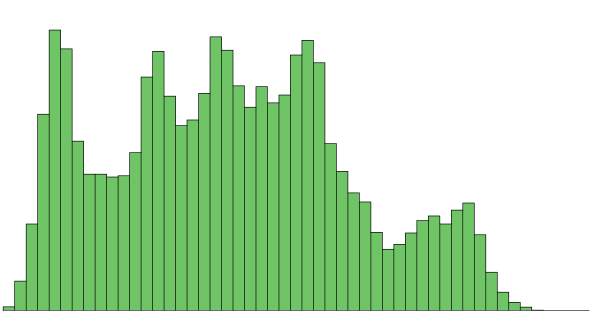
\includegraphics[width=0.25\linewidth,height=0.08\textheight]{Images/SVG/Lena_hist10} & \includegraphics[width=0.25\linewidth,height=0.08\textheight]{Images/SVG/Lena_hist11} & 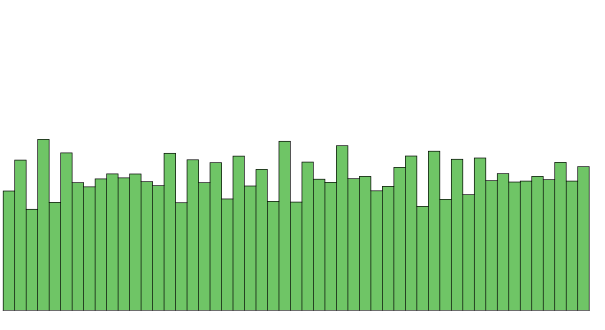
\includegraphics[width=0.25\linewidth,height=0.08\textheight]{Images/SVG/Lena_hist12}\tabularnewline
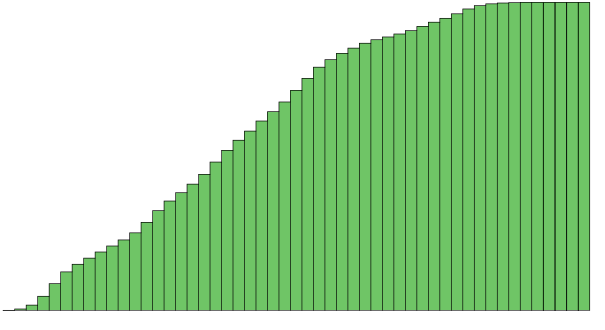
\includegraphics[width=0.25\linewidth,height=0.08\textheight]{Images/SVG/Lena_hist_cum10} & 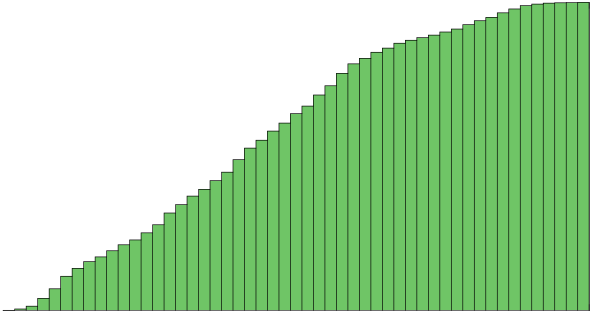
\includegraphics[width=0.25\linewidth,height=0.08\textheight]{Images/SVG/Lena_hist_cum11} & 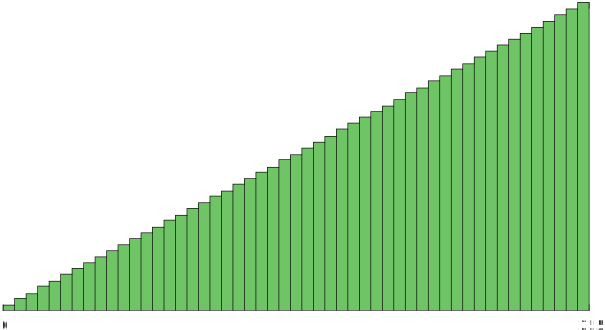
\includegraphics[width=0.25\linewidth,height=0.08\textheight]{Images/SVG/Lena_hist_cum12}\tabularnewline
\end{tabular}\caption{Ukázka roztažení a ekvalizace histogramu: \textbf{A)} originální obraz
a jeho histogram, \textbf{B)} obraz s roztaženým histogramem a \textbf{C)}
obraz s ekvalizovaným histogramem. V prvním řádku je obraz, ve druhém
jeho odhad hustoty pravděpodobnosti intenzity z histogramu a ve třetím
je odhad distribuční funkce intenzity z kumulativního histogramu.
\label{fig:Ekvalizace}}
\end{figure}


\section{Ekvalizace histogramu}

Jde o tzv. vyrovnání histogramu, resp. jako zploštění. Jasy se transformují
tak, aby každý z nich ,,měl pro sebe`` takovou část jasové osy,
jaké je jeho zastoupení v obrázku. Jako přechodníková funkce se používá
normovaný kumulativní histogram, tedy odhad distribuční funkce \prettyref{eq:CumHist_distr_fce}.
Dojde-li k tomu, že následující hodnota v histogramu pro danou intenzitu
převyšuje požadovanou hodnotu, nebo naopak požadované hodnoty nedosahuje,
je potřeba provést štěpení sloupců do více intenzit, případně sloučení
sloupců do jedné intenzity. Spojení sloupců problém není, ale jak
vysoké sloupce dělit? Používá se následující algoritmus (pro obrazy
s intenzitou v rozmezí $\left\langle 0,255\right\rangle $): Označme
počet pixelů obrazu $I$ písmenem $S$. Budeme procházet všechny intenzity
postupně od nejmenší po největší, tzn. od černé barvy po bílou. Pro
$k$-tou intenzitu najdeme všechny pixely v původním obrazu s danou
intenzitou, označme je $n_{k}$, a nastavíme jim novou intenzitu ve
tvaru 
\[
I_{new}=\textrm{round}\left[255\cdot\frac{n_{k}+2S_{k}}{2S}\right],
\]
kde $S_{k}$ je počet zpracovaných pixelů z předchozích kroků a $255$
značí intenzitu bílé barvy. Někdy se ekvalizuje i lokálně (změna jasu,
kontrastu), postup probíhá v okně podobně jako při konvoluci. Ukázka
ekvalizace histogramu a porovnání s obyčejným roztažením na všechny
možné intenzity je na obr. \ref{fig:Ekvalizace}.

\section{Šum}

Šum v obrázku je přidaná falešná informace nahodilého původu. Může
vznikat například při zpracování na senzoru fotoaparátu (prachové
částice), nebo při zpracování ve fotoaparátu (kvantizační šum). Abychom
si zjednodušili situaci, předpokládejme aditivní model šumu, neboli
na signálu nezávislý šum. Modelujeme jej pomocí funkce $n$
\[
f=f_{\mathrm{org}}+n.
\]
V našem diskrétním pojetí budeme uvažovat funkci $n$ jako náhodnou
veličinu, která měla $h\cdot w$ realizací ($h$ …výška obrazu, $w$
…šířka obrazu) nebo jako $h\cdot w$ náhodných veličin.
\begin{note}
Existuje i multiplikativní model šumu, tj. $f=f_{\mathrm{org}}\cdot n$.
\end{note}


\subsection{Bílý šum (AGWN)}

Situaci si zjednodušíme předpokladem bílého šumu (AGWN z anglického
\emph{Additive Gaussian White Noise}), což jsou nezávislé, stejně
rozdělené (iid) náhodné veličiny $X$, s normálním rozdělením (gaussovským)
a nulovou střední hodnotou, tj. $X\sim\text{\ensuremath{\mathcal{N}}}\left(0,\sigma^{2}\right)$.
Analogie s bílým světlem (bílé světlo obsahuje všechny frekvence)
plyne z nulové střední hodnoty a z toho, že míra šumu je stejná na
všech pixelech a pixel od pixelu nezávislá, tzn. šum jakožto náhodná
veličina na jednotlivých pixelech je nekorelovaný s šumem na ostatních
pixelech. Protože kovarianční matice jednoznačně zadává normální rozdělení,
tak je pro normální veličiny nekorelovanost to samé jako nezávislost.

Spočítejme \emph{power spektrum} naší šumové funkce. Power spektrum
odpovídá dle definice druhé mocnině amplitudového spektra Fourierovy
transformace šumové funkce $n$, tj. $PS=\left|N\right|^{2}$. Pokud
provedeme korelaci bílého šumu, dostáváme 
\begin{equation}
n\circledast n=\sigma_{n}^{2}\cdot\delta\quad\Longrightarrow\quad\mathcal{F}\left[n\circledast n\right]=\sigma_{n}^{2}.\label{eq:AGWN_corelation}
\end{equation}
Tento vztah plyne z vlastností šumu, tj. z nezávislosti. Z vlastností
Fourierovy transformace ovšem víme, že platí
\[
\mathcal{F}\left[n\circledast n\right]=N\cdot N^{\star}=\left|N\right|^{2}\quad\Longrightarrow\quad\left|N\right|^{2}=\sigma_{n}^{2},
\]
kde výslednou rovnost dostáváme díky vztahu (\ref{eq:AGWN_corelation}).
Vidíme, že power spektrum je rovno rozptylu, a je to tudíž konstantní
veličina, což je opět pro bílý šum charakteristické. V praxi by měla
při korelaci vzniknout matice, která je všude nulová, jen uprostřed
je hodnota rozptylu.

\subsection{Odstranění šumu}

Cílem je snížit rozptyl šumové funkce. Protože lidskému oku nejvíce
,,vadí`` vysoké frekvence šumu, provádí se tzv. \emph{nízkofrekvenční
filtr}ace, která tyto frekvence potlačuje. To s sebou nese nepříjemnou
vlastnost, že na vysokých frekvencích jsou zaznamenány i informace
o hranách, které se tímto způsobem rozmazávají.

\subsubsection{Lineární filtry (konvoluční filtry)}
\begin{enumerate}
\item \textbf{Průměrování v čase:} lze použít v případě, že je scéna statická,
tzn. nehýbe se. Uděláme $N$ nezávislých snímků dané scény $g_{1},g_{2},\ldots,g_{N}$,
sečteme v jednotlivých pixelech a vydělíme počtem snímků, tzn.
\[
g_{k}=f+n_{k}\quad\land\quad n_{k}\thicksim\mathcal{N}\left(0,\sigma_{n}^{2}\right)\quad\Longrightarrow\quad g=\frac{1}{N}\stackrel[k=1]{N}{\sum}g_{k}=f+\tilde{n}\quad\Longrightarrow\quad\tilde{n}\thicksim\mathcal{N}\left(0,\frac{\sigma_{n}^{2}}{N}\right).
\]
Šum klesá s hodnotou $\nicefrac{\sigma^{2}}{N}$ a navíc tato metoda
nepřináší žádné degradace.
\item \textbf{Průměrování:} používáme například konvoluční maticí $C$ (průměrování
prosté nebo vážené) 
\[
C=\frac{1}{9}\left(\begin{array}{ccc}
1 & 1 & 1\\
1 & 1 & 1\\
1 & 1 & 1
\end{array}\right)\qquad\text{nebo}\qquad C=\frac{1}{16}\left(\begin{array}{ccc}
1 & 2 & 1\\
2 & 4 & 2\\
1 & 2 & 1
\end{array}\right).
\]
\item \textbf{Průměrování podél hran:} podél hran používáme jiný druh filtru,
v ostatních částech obrazu používáme obyčejné průměrování. Pro použití
musíme mít apriorní informaci o hranách a to proto, že detektory hran
reagují na šum stejně jako na hrany.
\item \textbf{Metoda rotujícího okna:} v okolí daného bodu definujeme 8
oblastí pro všech 8 směrů. V každé této oblasti spočítáme rozptyl
a vybíráme oblast s nejmenším rozptylem. Ve vybrané oblasti spočítáme
průměr a nahradíme jím bod uprostřed masky. Tato metoda se dost používá
a dává dobré výsledky. Její výhodou je, že respektuje směr a umístění
hran. Nevýhodou je, že vytváří malé oblasti se stejnou intenzitou.
Tato charakteristická vlastnost je způsobena principem metody, protože
pokud vybereme oblast s nejmenším rozptylem, tak je pravděpodobné
, že s posunutím o jeden pixel bude vybrána ta samá oblast, a tedy
dosadíme stejný průměr. 
\begin{figure}[h]
\centering{}\include{Images/Metoda_rotujiciho_okna}\caption{Metoda rotujícího okna na okolí bodu velikosti $5\times5$.}
\end{figure}
\item \textbf{Filtry ve frekvenční oblasti:} ve frekvenční oblasti odstraníme
nebo utlumíme vysoké frekvence pomocí hladkých \emph{low-pass} filtrů.
\end{enumerate}
\begin{note}
Všechny tyto filtry mohou být kombinovány s prahováním, kdy výsledek
měníme pouze pokud konvoluce v bodě překročila zadaný práh.
\end{note}


\subsubsection{Nelineární filtry}
\begin{enumerate}
\item \textbf{Mediánový filtr:} v okně provedeme seřazení dat a prostřední
prvek (medián) dáváme do výsledku. Tato metoda potlačuje šum, ale
,,okusuje`` okraje a rohy, např pokud máme čáru širokou jeden pixel,
tak jí mediánový filtr ,,sežere``. Proto je vhodnější volit za výběrové
okno třeba kříž. Navíc pokud je zašuměných více než 50 \% pixelů,
metoda bere šum jako originální obrázek a šumu po filtraci ještě přibude.
Tento filtr je vhodnější na šum typu sůl a pepř. Při použití na bílý
šum moc dobře nefunguje.

Náročnost algoritmu pro symetrické okno šířky $n$ (tedy obsahující
$n^{2}$ prvků) by byla při použití algoritmu \emph{Quicksort} $O\left(n^{4}\right)$.
V případě použití algoritmu \emph{Heapsort} je náročnost $O\left(\left(n\log n\right)^{2}\right)$.
Pro další zrychlení lze využít vkládání do utříděné posloupnosti.
Novější algoritmus FMF (\emph{fast median filter}) pracuje při složitosti
$O\left(n\right)$. Urychlení je provedeno díky konstrukci a aktualizaci
histogramu, hledání mediánu je pak velmi rychlé.
\item \textbf{Zobecněný mediánový filtr:} v okně provedeme seřazení dat
a na setříděnou posloupnost aplikujeme váhovou funkci $w$ rovnu např.
\[
w=\frac{1}{4}\left(0,\dots,0,1,2,1,0,\dots,0\right).
\]
\end{enumerate}
Téměř všechny předchozí filtry lze použít i ve frekvenční oblasti.
Pokud víme, že má obraz jen jisté druhy hran (např. vodorovné), lze
použít speciální filtr (např. $\frac{1}{4}\left(1,1,1,1\right)$).
Ve frekvenční oblasti má pak tento filtr taktéž speciální tvar.

\subsubsection{Metody zachovávající hrany}

Jedná se např. o minimalizaci funkcionálu (funkcionál energie), anizotropní
difuzi a splainové metody.

\subsection{Šum typu sůl a pepř (\emph{salt \& pepper})}

Tento speciální druh šumu vzniká při pořizování obrázku na snímacích
zařízeních a je to tzv. impulsní šum. Většina bodů je správně načtená,
ale občas některý vypadne nebo se maximálně zesvětlí. Matematický
model pro tento šum je ve tvaru
\[
f_{i,j}=\left\{ \begin{array}{ccl}
I_{max} & \ldots & \text{s pravděpodobností }p,\\
\textrm{nemění se} & \ldots & \text{s pravděpodobností }1-p-q,\\
I_{min} & \ldots & \text{s pravděpodobností }q,
\end{array}\right.
\]
kde $r=p+q\in\mathcal{U}\left(0,1\right)$ udává míru zašumění, $I_{min}$,
$I_{max}$ je minimální a maximální možná intenzita a $f_{i,j}$ je
pixel obrazu na pozici $\left(i,j\right)$. Filtr, který tyto nesprávně
načtené body opravuje, je opět v podobě konvolučního filtru s maticí
tvaru 
\[
C=\frac{1}{8}\left(\begin{array}{ccc}
1 & 1 & 1\\
1 & 0 & 1\\
1 & 1 & 1
\end{array}\right)
\]
Aplikuje se pouze na tmavé a světlé body obrazu (v ostatních to nemá
smysl) a dává uspokojivé výsledky. Lze také použít mediánový filtr.
Pokud provádíme opakované snímání (např. sledujeme experiment v laboratoři),
používá se i triviální odstranění šumu pomocí průměrování více kopií.
Protože na každé kopii je jiná realizace šumu, tak v průměru vymizí.
Pokud je možnost takového snímání, pak se jedná o ideální způsob jak
šum odstranit.

\subsection{Periodické poškození obrazu}

Pokud se na obraze vyskytuje jisté periodické poškození (např. pohled
přes pletivo, mříže, fotka na vroubkovaném papíře), lze tyto ,,funkce``
z obrazu odstranit. Ve frekvenční oblasti totiž obdržíme amplitudové
spektrum s nápadnými symetrickými píky mimo střed. Když je odstraníme,
vymizí z obrazu i poškození, viz obr. \ref{fig:Periodicke_poskozeni}.
\begin{figure}[h]
\centering{}%
\begin{tabular}{ccc}
\textbf{A)} & \textbf{B)} & \textbf{C)}\tabularnewline
\includegraphics[width=0.2\linewidth]{Images/PNG/Lena_original} & \includegraphics[width=0.2\linewidth]{Images/PNG/Lena_poskozena} & \includegraphics[width=0.2\linewidth]{Images/PNG/Lena_restaurace}\tabularnewline
\textbf{D)} & \textbf{E)} & \textbf{F)}\tabularnewline
\includegraphics[width=0.2\linewidth]{Images/PNG/Lena_original_spektrum} & \includegraphics[width=0.2\linewidth]{Images/PNG/Lena_poskozena_spektrum} & \includegraphics[width=0.2\linewidth]{Images/PNG/Lena_restaurace_spektrum}\tabularnewline
\end{tabular}\caption{Periodické poškození:\textbf{ A)} originální obraz, \textbf{B)} obraz
s periodickým poškozením a \textbf{C)} výsledný restaurovaný obraz
a frekvenční spektra: \textbf{D)} originálního obrazu, \textbf{E)}
obrazu s periodickým poškozením a \textbf{F)} upravené spektrum obrazu
s periodickým poškozením. \label{fig:Periodicke_poskozeni}}
\end{figure}


\subsection{Kvantifikace šumu}

Pro měření ,,velikosti`` šumu v obraze se zavádí tzv. \emph{signal-to-noise
ratio }($SNR$), což je funkce definovaná jako 
\begin{equation}
SNR=\frac{\left|F\right|^{2}}{\left|N\right|^{2}}\left(u,v\right),\label{eq:SNR}
\end{equation}
kde $\left|N\right|^{2}$ a $\left|F\right|^{2}$ se nazývají výkonová
spektra (\emph{power spectrum}) .Tato funkce zachycuje tu vlastnost,
že šum nám vadí hlavně při vysokých frekvencích. Uvažujme velké zjednodušení
a předpokládejme, že obrázek není prostorově korelovaný, tj. $\left|F\right|^{2}=\sigma_{f}^{2}$,
a bílý šum, tj. $\left|N\right|^{2}=\sigma_{n}^{2}$. Tímto zjednodušením
dostáváme vztah 
\begin{equation}
SNR=\frac{\left|F\right|^{2}}{\left|N\right|^{2}}\left(u,v\right)=\frac{\sigma_{f}^{2}}{\sigma_{n}^{2}}\quad\forall u,v.\label{eq:SNR_bily_sum}
\end{equation}
Pro rozumnou práci zavádíme tzv. \emph{odstup signálu od šumu} ($snr$),
který měříme v decibelech {[}dB{]} a definujeme jej jako 
\[
snr=10\log_{10}\frac{\textnormal{Var}\left(f\right)}{\textnormal{Var}\left(n\right)}=10\log_{10}\frac{\sigma_{f}^{2}}{\sigma_{n}^{2}}.
\]
Čím vyšší je hodnota odstupu signálu od šumu, tím lepší (méně zašuměný)
máme signál. Pro oko je hodnota 15~dB dostačující. V praxi $\sigma_{n}^{2}$
a $\sigma_{f}^{2}$ většinou neznáme, takže je odhadujeme jako celek.

\section{Detekce hran}

Nejedná se již o předzpracování, spíše už se snažíme rozpoznat další
neobrazové informace. \emph{Hranou} pro nás bude výrazná změna intenzity
obrazu. Experimenty ukazují, že lidské oko se podle hran silně orientuje.
Ztráta hranové informace vede ke zmatení a chybám v interpretaci vjemu.
Detekce hran se realizuje několika způsoby, které jsou založeny na
sledování 1. derivace, resp. 2. derivace funkce intenzity.
\begin{figure}[h]
\centering{}\include{Images/Hrany_typy}\caption{Typy hran pro rozpoznávání v obraze: \textbf{A)} ideální hrana (\emph{step
edge}), \textbf{B)} typická pozvolná hrana (\emph{ramp edge}), \textbf{C)}
střechovitá hrana (\emph{roof edge}). }
\end{figure}


\subsection{Detektory používající první derivaci}

Tyto detektory hledají body, kde má první derivace maximum, tedy $\underset{x}{\arg\max}\left|\nabla f\left(x,y\right)\right|$.
Gradient funkce (obrazu) získáme aproximací
\begin{align*}
\nabla f\left(x,y\right) & =\left[\frac{\partial f\left(x,y\right)}{\partial x},\frac{\partial f\left(x,y\right)}{\partial y}\right], & \frac{\partial f\left(x,y\right)}{\partial x} & \sim\frac{f\left(x+\varepsilon,y\right)-f\left(x,y\right)}{\varepsilon}\sim f\left(x+1,y\right)-f\left(x,y\right),
\end{align*}
což odpovídá konvoluci s jádrem $C=\left(-1,1\right)$. 
\begin{figure}[h]
\centering{}%% Creator: Inkscape 0.91, www.inkscape.org
%% PDF/EPS/PS + LaTeX output extension by Johan Engelen, 2010
%% Accompanies image file 'Hrany_derivace.pdf' (pdf, eps, ps)
%%
%% To include the image in your LaTeX document, write
%%   \input{<filename>.pdf_tex}
%%  instead of
%%   \includegraphics{<filename>.pdf}
%% To scale the image, write
%%   \def\svgwidth{<desired width>}
%%   \input{<filename>.pdf_tex}
%%  instead of
%%   \includegraphics[width=<desired width>]{<filename>.pdf}
%%
%% Images with a different path to the parent latex file can
%% be accessed with the `import' package (which may need to be
%% installed) using
%%   \usepackage{import}
%% in the preamble, and then including the image with
%%   \import{<path to file>}{<filename>.pdf_tex}
%% Alternatively, one can specify
%%   \graphicspath{{<path to file>/}}
%%
%% For more information, please see info/svg-inkscape on CTAN:
%%   http://tug.ctan.org/tex-archive/info/svg-inkscape
%%
\begingroup%
  \makeatletter%
  \providecommand\color[2][]{%
    \errmessage{(Inkscape) Color is used for the text in Inkscape, but the package 'color.sty' is not loaded}%
    \renewcommand\color[2][]{}%
  }%
  \providecommand\transparent[1]{%
    \errmessage{(Inkscape) Transparency is used (non-zero) for the text in Inkscape, but the package 'transparent.sty' is not loaded}%
    \renewcommand\transparent[1]{}%
  }%
  \providecommand\rotatebox[2]{#2}%
  \ifx\svgwidth\undefined%
    \setlength{\unitlength}{328bp}%
    \ifx\svgscale\undefined%
      \relax%
    \else%
      \setlength{\unitlength}{\unitlength * \real{\svgscale}}%
    \fi%
  \else%
    \setlength{\unitlength}{\svgwidth}%
  \fi%
  \global\let\svgwidth\undefined%
  \global\let\svgscale\undefined%
  \makeatother%
  \begin{picture}(1,0.20731707)%
    \put(0.52439024,0.15853658){\color[rgb]{0,0,0}\makebox(0,0)[lb]{\smash{\footnotesize $\nabla f$}}}%
    \put(0.85951315,0.15853658){\color[rgb]{0,0,0}\makebox(0,0)[lb]{\smash{\footnotesize $\Delta f$}}}%
    \put(0,0){\includegraphics[width=\unitlength,page=1]{Hrany_derivace.pdf}}%
    \put(0.15853659,0.09756097){\color[rgb]{0,0,0}\makebox(0,0)[lb]{\smash{}}}%
    \put(0.13658537,0.09756097){\color[rgb]{0,0,0}\makebox(0,0)[lb]{\smash{\footnotesize $f$}}}%
  \end{picture}%
\endgroup%
\caption{Funkce $f$ obsahující hranu a její první a druhá derivace.}
\end{figure}


\subsubsection{Robertsův detektor:}

Jedná se o konvoluční filtr s maticemi
\begin{align*}
C & =\left(1,-1\right), & C & =\left(\begin{array}{c}
1\\
-1
\end{array}\right), & C & =\left(\begin{array}{cc}
1 & 0\\
0 & -1
\end{array}\right), & C & =\left(\begin{array}{cc}
0 & 1\\
-1 & 0
\end{array}\right),
\end{align*}
 pro všesměrovou detekci hran. Nevýhoda tohoto filtru je velikost
konvolučních masek, díky níž detekuje i šum jako hrany. Tato vada
je způsobena tím, že detektor používá derivaci jen v jednom bodě.
\begin{note}
Všesměrovou detekci realizujeme postupnou aplikací všech 8 konvolučních
masek, tj. získáním 8 hranových obrazů. Tyto hranové obrazy poté spojíme
dohromady za použití maximového pravidla, tzn. bereme vždy největší
hodnotu v daném pixelu ze všech 8 hranových obrazů. Pro zlepšení hranové
detekce se dále používá prahování. Tento postup všesměrové detekce
se používá i pro další konvoluční hranové filtry.
\end{note}


\subsubsection{Detektor Prewittové :}

Jistým vylepšením Robertsova detektoru je detektor Prewittové, který
pro detekci hran používá konvoluční masky ve tvaru
\begin{align*}
C & =\left(\begin{array}{ccc}
1 & 0 & -1\\
1 & 0 & -1\\
1 & 0 & -1
\end{array}\right), & C & =\left(\begin{array}{ccc}
1 & 1 & 0\\
1 & 0 & -1\\
0 & -1 & -1
\end{array}\right),
\end{align*}
a jejich obdoby pro další směry. 

\subsubsection{Sobelův detektor:}

Výhoda Sobelova detektoru proti Robertsovu detektoru je ta, že počítá
derivaci ze tří bodů (z centrálního bodu a bodů okolo). Je tedy robustnější
proti šumu. Má celkem 8 konvolučních masek ve tvaru
\begin{align*}
C & =\left(\begin{array}{ccc}
-1 & -2 & -1\\
0 & 0 & 0\\
1 & 2 & 1
\end{array}\right), & C & =\left(\begin{array}{ccc}
-2 & -1 & 0\\
-1 & 0 & 1\\
0 & 1 & 2
\end{array}\right).
\end{align*}
Konvoluční masky pro zbylých 6 směrů vznikají rotací a vypadají obdobně.
\begin{note}
Pokud nejprve obrázek vyhladíme (rozmažeme), a pak na něj aplikujeme
Sobelův detektor, dostaneme hranový obraz, který by vznikl aplikací
Robertsova detektoru na větší okolí, tzn. žádný lepší výsledek se
nedostaví
\[
C_{1}=\frac{1}{9}\left(\begin{array}{ccc}
1 & 1 & 1\\
1 & 1 & 1\\
1 & 1 & 1
\end{array}\right),\quad C_{2}=\left(\begin{array}{ccc}
-1 & -2 & -1\\
0 & 0 & 0\\
1 & 2 & 1
\end{array}\right)\quad\Longrightarrow\quad C_{3}=C_{1}\circ C_{2}=\left(\begin{array}{ccc}
- & - & -\\
0 & 0 & 0\\
+ & + & +
\end{array}\right),
\]
\[
\left(f\ast C_{1}\right)\ast C_{2}=f\ast C_{3}.
\]
\end{note}


\subsubsection{Kirschův detektor:}

Podobně jako Sobelův detektor tento detektor pracuje s 8 konvolučními
maskami, které jsou ve tvaru
\begin{align*}
C & =\left(\begin{array}{ccc}
5 & 5 & 5\\
-3 & 0 & -3\\
-3 & -3 & -3
\end{array}\right), & C & =\left(\begin{array}{ccc}
5 & 5 & -3\\
5 & 0 & -3\\
-3 & -3 & -3
\end{array}\right).
\end{align*}
Konvoluční masky pro zbylých 6 směrů vznikají rotací a vypadají obdobně.
Všesměrová detekce probíhá stejně jako u Sobelova detektoru.

\subsubsection{Cannyho detektor.}

Používá se velmi často. Byl vytvořen s požadavky aby detekoval všechny
hrany, každou hranu detekoval právě jednou a přesně ji lokalizoval
(střed hrany) a aby nevytvářel hrany navíc. Princip Cannyho detektoru
je následující:
\begin{enumerate}
\item Odstranění šumu vyhlazením pomocí konvoluce s Gaussovým jádrem.
\item Výpočet parciálních derivací, stačí i jednoduchý detektor, např. \emph{Roberts
Cross function} 
\[
\left|\begin{array}{cc}
1 & 0\\
0 & -1
\end{array}\right|.
\]
Dále se provede ,,\emph{non-maximum suppression}``. Úkolem této
procedury je vybrat z hodnot gradientů (stanovených v předchozím kroku)
jen lokální maxima. Respektive odebrat body, které nejsou maximem
(,,detekce hřbetů``), čímž zajistíme, že hrana bude detekována v
místě největšího gradientu.
\item Prahování s hysterezí (\emph{Double threshold}). V předchozím kroku
jsme určili, kde přesně leží hrany, ale doposud jsme se nezabývali
jejich významem. V tuto chvíli jsou označeny i ty nejmenší hrany,
protože i ty mají své lokální maximum. Zvolíme minimální $t_{min}$
a maximální $t_{max}$ práh, mezi kterými může gradient kolísat. Pokud
hodnota gradientu daného pixelu leží nad větším prahem $t_{max}$
je označen jako \emph{silný}. Pokud posuzujeme bod, jehož hodnota
leží mezi $t_{min}$ a $t_{max}$, je označen jako \emph{slabý. }Silné
pixely zachováváme vždy a slabé zachováváme, pokud sousedí se silným
pixelem.
\end{enumerate}
Cannyho detektor je tvořen sadou odvozených filtrů, které závisí na
parametrech. Nastavením parametrů lze docílit výborných výsledků.

\subsection{Detektory používající druhou derivaci\label{subsec:Detektory_druhou_derivace}}

Tyto detektory hledají body, kde má druhá derivace průchod nulou.
Pro druhou derivaci platí 
\[
\frac{\partial}{\partial x^{2}}=\left(-1,1\right)\ast\left(-1,1\right)=\left(1,-2,1\right)
\]
z čehož lze odvodit tvar Laplaceova operátoru 
\[
\Delta=\frac{\partial}{\partial x^{2}}+\frac{\partial}{\partial y^{2}}=\left(\begin{array}{ccc}
0 & 0 & 0\\
1 & -2 & 1\\
0 & 0 & 0
\end{array}\right)+\left(\begin{array}{ccc}
0 & 1 & 0\\
0 & -2 & 0\\
0 & 1 & 0
\end{array}\right)=\left(\begin{array}{ccc}
0 & 1 & 0\\
1 & -4 & 1\\
0 & 1 & 0
\end{array}\right).
\]
 Neřešíme tedy rovnici $\Delta f=0$, ale hledáme, zda se v $\Delta f$
objevují velké přechody mezi kladnou a zápornou hodnotou (tzv. \emph{zero-crossing
points}). V těchto místech pak zaznamenáme hranu. Tento způsob je
velmi náchylný na šum (dokonce víc než Robertsův detektor).

\subsubsection{Marr Hildrethův detektor (LoG):\label{subsec:Marr}}

Marr a Hildreth navrhli modifikaci, při které se sleduje funkce 
\[
\Delta\left(G\ast f\right)=\Delta G\ast f,
\]
kde $G$ je kruhově symetrická Gaussova funkce. Matice $\Delta G$
se předpočítává a bývá široká $5\times5$ až $15\times15$ pixelů.
Parametrizací Gaussovy funkce lze docílit výborných výsledků. Širší
funkce detekuje podstatné hrany a je méně náchylná na šum, užší se
chová jako předchozí detektory. Detektor má tendenci vytvářet uzavřené
hrany (křivky). Tento fakt plyne z teorie Laplaceových operátorů a
řešení Laplaceovy rovnice $\Delta f=0$. Pro lokalizaci hrany se často
používá místo složitějšího hledání ,,průchodu nulou`` jednoduché
nalezení $\max\left|\Delta f\right|$, viz obr. \ref{fig:Zero_cross_point}.
\begin{figure}[h]
\centering{}\include{Images/Hrany_prusecik}\caption{\label{fig:Zero_cross_point}Hledání \emph{zero-crossing point} pomocí
$\max\left|\Delta f\right|$.}
\end{figure}
 

\subsection{Detektory nepoužívající derivace}

\subsubsection{Whitening}

Tato metoda spočívá v tom, že amplitudy Fourierovy transformace nahradíme
konstantní funkcí. Zůstává nám tím harmonická informace. Poté provedeme
konvoluci s maskou $C$, a tím docílíme, že hrany zůstanou jen v určitém
směru. Budeme ztrácet informaci o hranách s větší šířkou.

\subsection{Detektory pracující ve frekvenční oblasti}

Chceme-li ve frekvenční oblasti detekovat hrany pod určitým úhlem,
musíme se ve spektru signálu dívat ve směru kolmém na tento úhel.
Po převedení do frekvenční oblasti lze využít směrových filtrů, viz
obr. \ref{fig:Filtry_frekvencni}.

\subsection{Zvýraznění hran}

Abychom při hledání hran dosahovali lepších výsledků, můžeme před
samotnou detekcí hrany zvýraznit.
\begin{itemize}
\item Jednou z možností je použití konvoluce. Celkem potřebujeme masky pro
4 směry, které jsou ve tvaru
\begin{align*}
C & =\left(\begin{array}{ccc}
-1 & -1 & -1\\
2 & 2 & 2\\
-1 & -1 & -1
\end{array}\right), & C & =\left(\begin{array}{ccc}
2 & -1 & -1\\
-1 & 2 & -1\\
-1 & -1 & 2
\end{array}\right),
\end{align*}
a pro zbylé 2 směry obdobně. Po konvoluci se ještě provádí prahování
maximálních hodnot.
\item Další možností je použití Laplaceova operátoru $\Delta$ (odvození
tvaru Laplaceova operátoru viz sekce \ref{subsec:Detektory_druhou_derivace}).
Hrany zvýrazníme odečtením Laplaceova operátoru od funkce $f-\Delta f$.
Při použití aproximace to odpovídá konvoluci s maskou $C$, tzn.
\[
f-\Delta f\quad\Longrightarrow\quad\left(\begin{array}{ccc}
0 & 0 & 0\\
0 & 1 & 0\\
0 & 0 & 0
\end{array}\right)-\left(\begin{array}{ccc}
0 & 1 & 0\\
1 & -4 & 1\\
0 & 1 & 0
\end{array}\right)\quad\Longrightarrow\quad C=\left(\begin{array}{ccc}
0 & -1 & 0\\
-1 & 5 & -1\\
0 & -1 & 0
\end{array}\right).
\]
\item Poslední metodou jak zvýraznit hrany je tzv. neostré maskování (\emph{unsharp
masking}). Nejdříve odečteme od originálního signálu vyhlazený signál
$f_{smooth}$ pomocí \emph{low-pass} filtru čímž získáme \emph{high-pass}
reprezentaci $f_{high}$. Pokud \emph{high-pass} reprezentaci přičteme
k původnímu signálu, dostáváme ,,zaostřený `` signál $f_{sharp}$
\begin{alignat*}{1}
\ensuremath{f_{high}\left(x,y\right)} & =f\left(x,y\right)-f_{smooth}\left(x,y\right),\\
\ensuremath{f_{sharp}\left(x,y\right)} & =f\left(x,y\right)+k\cdot f_{high}\left(x,y\right),
\end{alignat*}
kde $k$ je škálovací konstanta. Na obr. \ref{fig:Neostre_maskovani}
je zobrazen princip neostrého maskování.
\begin{figure}[h]
\centering{}\include{Images/Neostre_maskovani}\caption{Princip neostrého maskování: \textbf{A) }originální signál, \textbf{B)
}vyhlazený signál, \textbf{C)} \emph{high-pass} reprezentaci, \textbf{D)}
,,zaostřený `` signál. \label{fig:Neostre_maskovani}}
\end{figure}
\end{itemize}

\section{Houghova transformace}

Jedná se o metodu nalezení parametrického popisu objektů v obraze.
Abychom metodu mohli použít, je třeba znát analytický popis hledaných
objektů. Je to tedy vhodná metoda na detekci jednoduchých objektů,
jako např. přímka, kruh, elipsa, případně objektů, jejichž hranici
lze popsat jednoduchými křivkami. 

Každá přímka lze popsat pomocí úhlu $\theta$, který svírá kolmice
na přímku procházející středem souřadné soustavy s osou souřadné soustavy,
a vzdálenosti $r$ přímky od počátku souřadné soustavy. Z tohoto popisu
lze odvodit vztah
\[
r=x\cdot\cos\theta+y\cdot\sin\theta.
\]
Máme tedy vztah, kterým můžeme z klasické souřadné soustavy přejít
do soustavy tvořené dvojicí proměnných $r$ a $\theta$, která se
nazývá Houghův prostor. Pokud provedeme tuto transformaci, tak se
nám přímka promítne na bod. Bod se promítne na křivku, která reprezentuje
všechny přímky procházející daným bodem v klasické souřadné soustavě.
Průsečíky křivek v Houghově prostoru reprezentují přímky. Fungování
Houghovy transformace je znázorněno na obr. \ref{fig:Hough}.

Pokud tedy chceme hledat hrany pomocí této transformace, tak provedeme
transformaci pro celý obraz a v Houghově prostoru hledáme průsečíky,
které reprezentují přímku. Většinou nelze kvůli deformací nalézt přímo
jednoznačný průsečík, a tak hledáme shluky bodů. To je také největší
problém metody.
\begin{figure}[h]
\centering{}%
\begin{tabular}{ccccc}
\multicolumn{2}{c}{\textbf{A)}} &  & \multicolumn{2}{c}{\textbf{B)}}\tabularnewline
\includegraphics[height=0.15\textheight]{Images/PNG/Hough_org13} & \includegraphics[height=0.15\textheight]{Images/PNG/Hough_tra13} & \hspace{1cm} & \includegraphics[height=0.15\textheight]{Images/PNG/Hough_org14} & \includegraphics[height=0.15\textheight]{Images/PNG/Hough_tra14}\tabularnewline
\end{tabular}\caption{Houghova transformace působící na body \textbf{A)}, resp. přímku \textbf{B)}.\label{fig:Hough}}
\end{figure}


\chapter{Restaurace obrazu\label{chap:Restaurace-obrazu}}

Nyní se zabývejme modelováním jiné než šumové degradace vzorového
obrazu. Zajímat nás bude hlavně konvoluční degradace. Nechť $g$ je
náš obraz, $f$ bude ideální, nezkreslený obraz (originál). Symbol
$\mathcal{D}$ bude značit \emph{operátor degradace} a $n$ aditivní
šum. Obecně případ modelujeme vztahem $g=\mathcal{D}(f)$. Předpokládejme
speciální volbu operátoru $\mathcal{D}$ ve tvaru 
\[
\mathcal{D}=\mathcal{T}_{G}\circ\mathcal{T}_{I},
\]
kde $\mathcal{T}_{G}$ je \textbf{\emph{geometrická degradace}} a
$\mathcal{T}_{I}$ je \textbf{\emph{radiometrická degradace}}. Výsledný
model lze zapsat ve tvaru 
\[
g=\mathcal{T}_{G}\circ\mathcal{T}_{I}(f)+n.
\]


\section{Radiometrické zkreslení (radiometrický inverzní problém)}

Pokud nepředpokládáme geometrické zkreslení a uvážíme, že ve většině
běžně dostupných zobrazovacích systémů lze $\mathcal{T}_{I}$ modelovat
pomocí konvoluce, můžeme vztah přepsat na tvar
\begin{equation}
g=f\ast h+n.\label{eq:RI_problem_model}
\end{equation}
Funkce $h$ se zde označuje jako \emph{impulsní odezva} a jedná se
o tzv. \emph{point spread function} (polohově invariantní) funkci.\footnote{Lze ji získat třeba vyfocením bodu: $\delta*h=h$ $\implies$ výstup
je \emph{point spread function}.} Polohová invariance značí skutečnost, že výsledek vztahu ovlivňující
dva pixely není závislý na jejich poloze, ale pouze na jejich vzájemné
vzdálenosti.\footnote{Toto je příliš velké omezení pro 3D scény, kde se rozmazání mění s
hloubkou ostrosti.}

\subsection{Inverzní filtr}

Rovnici \prettyref{eq:RI_problem_model} můžeme převést do frekvenční
oblasti Fourierovou transformací a dostaneme
\begin{equation}
G=F\cdot H+N\quad\Longrightarrow\quad F=\frac{G-N}{H}=\frac{G}{H}-\frac{N}{H},\label{eq:RI_problem_FT}
\end{equation}
kde dělení provádíme po složkách. Nulové body v $H$ můžou následně
vadit při inverzní Fourierově transformaci, proto provádíme bilineární
interpolaci funkce $F$ z nejbližšího okolí v místech, kde bylo $H$
nulové. Funkce $H$ se označuje jako \emph{přenosová funkce}. Pokud
známe $h$, lze navrhnout \emph{inverzní filtr} ve frekvenční oblasti
a po inverzní Fourierově transformaci dostáváme odhad originálu následovně
\[
\hat{f}=\mathcal{F}^{-1}\left[F\right]=\mathcal{F}^{-1}\left[\frac{G}{H}-\frac{N}{H}\right].
\]
V modelu bez šumu zanedbáváme ve vztahu \prettyref{eq:RI_problem_FT}
člen $\nicefrac{-N}{H}$ a v takovém případě inverzní filtr funguje
velmi dobře. Pro model se šumem může mít ovšem člen $\nicefrac{-N}{H}$
velmi zásadní vliv na výsledek, a to i pro malá $n$, jak ukazuje
graf na obr. \ref{fig:RI_problem}. Z tohoto důvodu je volba inverzního
filtru pro model se šumem nepoužitelná.
\begin{figure}[h]
\centering{}\include{Images/Inverzni_filtr}\caption{Hodnoty funkcí $H(x)$, $N(x)$ a jejich podílu. \label{fig:RI_problem}}
\end{figure}
 

\subsection{Wienerův filtr}

Místo inverzního filtru se pro zašuměný obrázek používá filtr Wienerův.
Požadavkem na Wienerův filtr $W$ bylo, aby byl lineární, tzn. ve
tvaru 
\begin{equation}
\hat{F}=G\cdot W,\label{eq:Wiener_pozadavek}
\end{equation}
a získaný odhad originálního obrazu byl co nejlepší. Předpis pro matici
$W$ dostaneme řešením minimalizační úlohy
\begin{equation}
W=\underset{\hat{f}}{\arg\min}\mathbb{E}\left[\|f-\hat{f}\|^{2}\right],\label{eq:Wiener_min}
\end{equation}
kde $f$ je originální obraz a $\hat{f}$ je odhad obrazu po rekonstrukci.
Minimalizaci provádíme přes všechny \textbf{lineární filtry}, a střední
hodnota je brána přes všechny možné realizace šumu. Matice $W$ není
přesně daná, je to funkce obrazu! Po netriviálním odvození dostaneme
výslednou matici $W$ ve tvaru
\[
W=\frac{1}{H}\cdot\frac{\left|H\right|^{2}}{\left|H\right|^{2}+SNR^{-1}\left(u,v\right)},
\]
kde funkce $SNR\left(u,v\right)$ značí \emph{signal-to-noise ratio},
viz \prettyref{eq:SNR}. Druhý člen v uvedením součinu je tzv. korekční
člen, který potlačuje frekvence, kde převládá šum. Pokud neznáme $\left|F\right|$
a $\left|N\right|$ (většinou neznámé), můžeme zkusit uvažovat bílý
šum a nekorelovanost původního obrazu, viz \prettyref{eq:SNR_bily_sum}
. V takovém případě tedy máme $SNR$ konstantní ve tvaru 
\[
SNR\left(u,v\right)=\frac{\sigma_{f}^{2}}{\sigma_{n}^{2}}=\text{const}\quad\forall u,v.
\]
Dále z nekorelovanosti původního obrazu platí
\[
f\circledast f=\delta\left(x\right)\sigma_{f}^{2}=\left\{ \begin{array}{ccc}
\sigma_{f}^{2}\cdot\delta(0) & \ldots & \text{pokud leží přesně na sobě},\\
0 & \ldots & \text{jinde}.
\end{array}\right.
\]
Při odhadování $SNR$ postupujeme tak, že s hodnotou $SNR$ začínáme
na nízké úrovni $\sim10^{-3}$ a postupně ji zvyšujeme třeba do $\sim10^{3}$
a sledujeme, co se děje s obrazem. Když Wienerův filtr aplikujeme
na nezašuměný obrázek (tedy $\left|N\right|^{2}=0$), pak matice $W$
přechází do tvaru $W=\nicefrac{1}{H}$ a celkem získáváme jednoduchý
inverzní filtr.

Pokud $SNR$ při rekonstrukci nadhodnotíme, tak dojde k zvýraznění
šumu. V případě podhodnocení $SNR$ dojde k rozostření obrazu, protože
potlačíme více vyšších frekvencí. 

\subsection{Základních typy radiometrických degradací}

Nyní se budeme zabývat odhadem přenosové funkce $H$ pro Wienerův
filtr. Impulsní odezva $h$ je neznámá a navíc může být ve tvaru $h=h_{1}\ast h_{2}\ast h_{3}\ast\dots$.
Obecně impulsní odezvu nelze zjistit. Můžeme ji pouze předpokládat
ve speciálních tvarech. Reálně rozlišujeme tři základní druhy degradace:
rozmazání pohybem, špatné zaostření a turbulence. Obvykle jsou zastoupeny
všechny základní degradace najednou, ale jedna výrazně převládá, a
ostatní tedy můžeme zanedbat.

\subsubsection{Rozmazání pohybem}

Je-li pohyb lineární (tj. po přímce), má impulsní odezva tvar obdélníka.
Předpokládejme konstantní rychlost pohybu, jinak je situace obtížná,
protože se vytrácí polohová invariance. V takovém případě je délka
obdélníku úměrná délce expozice a šířka je převrácená hodnota délky,
abychom zachovali $\int h=1$ a nevnášeli tak do obrazu jas. Ve směru
kolmém na směr pohybu se tento obdélník chová jako $\delta$-funkce,
a tedy nic nemění. Po Fourierově transformaci obdržíme ve frekvenční
oblasti známou funkci $\text{sinc}\left(t\right)=\nicefrac{\sin\left(\pi t\right)}{\pi t}$,
natočenou do směru pohybu. Slangově se tato funkce označuje jako \emph{vlnitý
plech}, viz obr. \ref{fig:FT_2D_signaly} a obr. \ref{fig:FT_2D_signaly_ve_3D}.

Nulové hodnoty funkce $H$ budou ležet na přímkách kolmých na směr
pohybu, viz obr. \ref{fig:Degradace_prehled}. Čím blíže budou nulové
body k sobě, tím je rozmazání větší. Stejné nulové body budou zachovány
i ve funkci $G$. Můžeme tak najít směr a délku pohybu (během expozice). 

Podobně lze odhadovat impulsní odezvy i na jiné druhy pohybu (např.
dítě na houpačce). Některé druhy pohybů lze převést na známé užitím
souřadnicové transformace. Třeba rotační pohyb gramofonové desky při
snímání shora převedeme na pohyb lineární s konstantní (úhlovou) rychlostí
pomocí radiálních souřadnic.

\subsubsection{Špatné zaostření (defokusace)}

Ideálním rozostřením světelného bodu je kruh. Ve skutečnosti ovšem
klesá jeho intenzita ke krajům. Impulsní odezva je tvaru válce a přenosová
funkce je ve tvaru
\begin{equation}
H\sim\frac{1}{r}J_{1}\left(r\right),\label{eq:Bessel}
\end{equation}
kde $J_{1}(r)$ je Besselova funkce 1. druhu a $r$ je radiální souřadnice,
viz obr. \ref{fig:FT_2D_signaly} a obr. \ref{fig:FT_2D_signaly_ve_3D}.
Díky výrazu $\nicefrac{1}{r}$ ve vztahu \prettyref{eq:Bessel} jsou
Besselovy kmity tlumené. Nulové body přenosové funkce jsou na soustředných
kružnicích, viz obr. \ref{fig:Degradace_prehled}. Stejné nulové body
budou zachovány i ve funkci $G$. Postup je obdobný jako v případě
lineárního posunutí. Změříme-li vzdálenost kružnic, můžeme odhadnout
impulsní odezvu.

\subsubsection{Turbulence}

Vzniká např. při snímání přes tlustou vrstvu atmosféry s delší expoziční
dobou, než je perioda Brownova pohybu částic v atmosféře. Impulsní
odezva, a tedy i přenosová funkce, jsou Gaussovy funkce, viz obr.
\ref{fig:FT_2D_signaly} a obr. \ref{fig:FT_2D_signaly_ve_3D}. Nemají
tedy nulové body, a nelze proto použít metodu z předchozích případů.
K odhadu se používají body, které nemění polohu, např. hvězdy ve snímcích
oblohy (astronomie). 
\begin{figure}[h]
\centering{}%
\begin{tabular}{c}
\includegraphics[width=12cm]{Images/PNG/Typy_degradace}\tabularnewline
\includegraphics[width=8.9cm]{Images/PNG/Typy_degradace_spektrum}\tabularnewline
\end{tabular} \caption{Základní typy degradací. Nahoře zleva původní obrázek, obrázek rozmazaný
pohybem, defokusací a turbulencí. Dole FT příslušné impulzní odezvy.\label{fig:Degradace_prehled}}
 
\end{figure}


\subsection{Problém slepé dekonvoluce}

V obecném případě pro neznámé $h$ nemá úloha jednoznačné řešení.
Zavádíme proto dodatečné omezující podmínky, které nám řešení zjednoduší,
např. nezápornost originálního signálu (snímku), omezenost nosiče
$h$ a minimalizace jistého potenciálového funkcionálu výsledného
obrazu.

Jiným problémem je tzv. \emph{vícekanálová slepá dekonvoluce}, kdy
máme k dispozici několik stejných snímků s jinými impulsními odezvami,
tzn. 
\begin{align*}
g_{1} & =f\ast h_{1}+n_{1},\\
 & \vdots\\
g_{k} & =f\ast h_{k}+n_{k}.
\end{align*}
Tato úloha je nepoměrně snazší, protože máme daleko více informací
a z každého $g_{i}$ jsme schopni zrekonstruovat jiné části obrázku.
Výsledek tedy můžeme ,,poslepovat`` z několika takových částí. Také
jsme schopni daleko lépe odstraňovat případné šumy, podobně jako při
průměrování více kopií.

\section{Geometrické zkreslení (geometrický inverzní problém)}

Model geometrického zkreslení obrazu lze zapsat jako 
\[
g=T_{G}\left(f\right).
\]
Máme-li snímek téže scény z různých pohledů (tj. s jiným geometrickým
zkreslením) a potřebujeme-li zjistit odpovídající pixely (tj. aby
stejné pixely měly stejné souřadnice), mluvíme o \emph{registraci
obrazu (image registration)}. Využití spočívá např. v detekci časových
změn. Nepřesná registrace vede na chybnou detekci, resp. zjištění
změn tam, kde nejsou. Rozlišujeme čtyři základní kategorie registrace
obrazu.
\begin{itemize}
\item Vícepohledová (\emph{different viewpoints, multi-view}).
\item Vícečasová (\emph{different times, multi-temporal}).
\item Multimodální (\emph{different modalities, multi-modal}).
\item Napasování scény na model registrace \emph{(scene to model registration).}
\end{itemize}
\noindent Registrace se provádí pomocí řídících bodů (\emph{control
points}). Pokud jsou správně nalezeny odpovídající řídící body v obou
obrazech, je možné sestavit geometrické transformace a snímky registrovat.
Postup registrace lze rozdělit do čtyř kroků, kterým se věnuje další
část textu. 

\subsection{Výběr kandidátů na řídící body (\emph{Control point selection})}

Na řídící body klademe základní požadavky a to, aby jich byl dostatečný
počet, byly rozmístěny po celém obraze, aby byly dobře automaticky
detekovatelné v obou obrazech a aby byly invariantní vůči transformaci.
Jako významné řídící body se volí \emph{rohy}, \emph{průsečíky }(citlivé
na šum), \emph{těžiště uzavřených oblastí} (na šum více stabilní),
nebo \emph{extrémní křivosti křivek}. V prvním kroku registrace se
řídící body vybírají zvlášť na referenčním obrazu a na registrovaném
obrazu. Ve druhém kroku je poté třeba provést vzájemnou korespondenci.
K tomuto účelu musíme mít dostatečně robustní, spolehlivou metodu,
neboť některé body mohou chybět, mohlo dojít k nepřesnostem atp.

\subsection{Korespondence řídících bodů (\emph{Control point matching})}

Jak už bylo řečeno, druhým krokem výběru řídících bodů, je nalezení
vzájemné korespondence mezi kandidáty na řídící body v referenčním
a registrovaném obrazu. Na základě korespondence kandidátů poté volíme
vhodné řídící body. Hledání odpovídajících si bodů se provádí buď
topologicky (předpokládaný výskyt), nebo se prohledává okolí bodu
s ohledem na intenzity (barvy) okolních pixelů. Rozlišujeme dva základní
druhy metod.

\subsubsection{Signálově závislé metody}

Tyto metody pracují s intenzitou obrázku. 
\begin{enumerate}
\item \textbf{Obrazová korelace:} korelaci provádíme se skutečnými obrazovými
hodnotami. Jeden obraz (okno) posouváme po druhém a počítáme korelaci.
Pokud existuje větší či menší shoda obrazů, bude na daném bodě ve
výsledné matici vysoká hodnota. Při konstantní korelační matici pak
tento postup odpovídá počítání dle vztahu 
\[
C\left(X,Y\right)=\frac{\mathbb{E}\left[\left(X-\mathbb{E}X\right)\left(Y-\mathbb{E}Y\right)\right]}{\sqrt{\text{Var}\left(X\right)}\cdot\sqrt{\text{Var}\left(Y\right)}}=\frac{\sum\limits _{i=0}^{N-1}\sum\limits _{j=0}^{N-1}\left(X_{ij}-\bar{X}\right)\cdot\sum\limits _{i=0}^{N-1}\sum\limits _{j=0}^{N-1}\left(Y_{ij}-\bar{Y}\right)}{\sqrt{\sum\limits _{i=0}^{N-1}\sum\limits _{j=0}^{N-1}\left(X_{ij}-\bar{X}\right)^{2}}\cdot\sqrt{\sum\limits _{i=0}^{N-1}\sum\limits _{j=0}^{N-1}\left(Y_{ij}-\bar{Y}\right)^{2}}}.
\]
V této podobě se metoda tolik nepoužívá, protože je výpočetně a časově
náročná a maximum bývá někdy ,,ploché``. Urychlení výpočetní složitosti
plyne z \emph{Korelačního teorému} 
\[
\mathcal{F}\left[f\circledast g\right]=F\cdot G^{\star},
\]
kde symbol $(\cdot)^{\star}$ značí komplexně sdruženou matici. Dále
lze provádět modifikace: korelace hran, rohů, korelace ve frekvenční
oblasti (fázová korelace), pyramidální reprezentace (\emph{pyramidal
representation}).

Metoda funguje dobře pro obrazy se stejnou intenzitou nebo pokud došlo
ke globálním změnám kontrastu a jasu. Ostatní změny dost vadí. V základním
provedení by metoda fungovala jen pro posun. Provádí se modifikace,
kdy je korelační matice trojrozměrná. Časová náročnost je ale příliš
veliká, proto se tato modifikace používá pouze pro malé rotace.

U této metody se většinou nedetekují řídící body v druhém obrázku,
ale hledají se nejvyšší korelace vzhledem k řídícím bodům prvního
obrázku. Nejčastěji hledáme malý výřez na velkém obrázku. Hodnoty
intenzit se liší pouze lineárně. Metoda dává dobré výsledky po hranové
detekci v obou obrazech.
\item \textbf{Fázová korelace:} Fáze Fourierovy transformace je blízká hranám
obrázků. Ty jsou výhodnější kvůli nezávislosti na barvách a mají menší
prostorovou korelaci. Nevrací se do obrazové oblasti pro počítání
korelace, ale zůstane se ve frekvenční oblasti, kde se využívá \emph{Fourier
Shift Theorem} (FST), viz věta \ref{thm:Fourier_Shift_Theorem}. Předpokládáme-li,
že první a druhý obrázek jsou stejné, ale jen posunuté, máme dány
funkce $f\left(\vec{x}\right)$ a $g\left(\vec{x}\right)=f\left(\vec{x}-\vec{a}\right)$,
kde $\vec{x},\vec{a}\in\mathbb{R}^{2}$. Po Fourierově transformaci
získáváme vztahy 
\begin{align*}
f\left(\vec{x}\right) & \stackrel{\mathcal{F}}{\longrightarrow}F\left(\vec{u}\right), & g\left(\vec{x}\right) & \stackrel{\mathcal{F}}{\longrightarrow}e^{-2\pi i\vec{u}\cdot\vec{a}}F\left(\vec{u}\right),
\end{align*}
kde $\vec{u}\cdot\vec{a}$ značí standardní skalární součin. Amplituda
je u obou Fourierových obrazů stejná, ale fáze se změnila známým způsobem.
Definujeme tzv. \emph{Cross-power} spektrum jako 
\[
\frac{F\cdot G^{\star}}{|F||G|}=\frac{\left|F\right|^{2}e^{2\pi i\vec{a}\cdot\vec{u}}}{\left|F\right|^{2}}\quad\stackrel{\mathcal{F}^{-1}}{\longrightarrow}\quad\delta\left(\vec{x}-\vec{a}\right).
\]
Tím vznikne dobře lokalizovatelný pík. Metoda funguje dobře, odpovídá
vlastně detekci hran a korelaci v obrazové oblasti.
\item \textbf{Nepodobnost (SSDA):} označuje se také jako ,,klasická korelace``.
Jde o použití jiné míry podobnosti než korelace, tzn. ne $L_{2}$
norma, ale $L_{1}$ norma, např. $\sum\left|f_{ij}-g_{ij}\right|$.
 Hledáme bod, kde norma nabývá minima. Výpočet je velmi rychlý, protože
suma je neklesající, jakmile tedy jednou částečný součet převýší již
vypočtené minimum, lze přímo přejít k dalšímu bodu.
\end{enumerate}
\begin{note}
Pro snadnou hardwarovou implementaci korelace jsou tyto metody (Fázová
korelace a nepodobnost (SSDA)) dosti používané.
\end{note}

\begin{note}
Lze rozšířit na obecnější transformace, např. pro rotaci je okénko
kruh. V takovém případě se ale stává úloha výpočetně velice náročná.
Dá se nejdříve projet prostým posunutím tam, kde je nalezeno maximum,
tak to začneme natáčet. Vybereme úhel natočení, kde je korelace maximální,
a poté projdeme opět celý obrázek s tímto natočením.
\end{note}

\begin{enumerate}
\item[4.] \textbf{ Pyramidální reprezentace:} Snižujeme rozlišení obrázků o
dvojnásobek. Začínáme na nízkém rozlišení, kde najdeme ,,nadějné
body`` a u vyššího rozlišení počítáme jen v okolí těchto bodů.
\end{enumerate}

\subsubsection{Příznakové metody (signálově nezávislé) (???)}

Jde o napočítávání vlastností \emph{(příznaků)} segmentovaných objektů
obrazu. Příznaky by měly být invariantní k transformaci, kterou předpokládáme.
Více o příznacích viz kapitola \ref{sec:Priznaky}.
\begin{enumerate}
\item \textbf{\emph{Point-based method}}\textbf{:} pro zjištění korespondence
řídících bodů se vytváří úplný graf a hledají se 4 parametry pro geometrickou
transformaci ($2\times$posun, $1\times$rotace, $1\times$měřítko).
Porovnáváme po dvojici hrany grafu a zjišťujeme, jak ostatní body
padají do okolí řídících bodů. Další možností je provést matching
a zaznamenávat do parametrického prostoru provedenou transformaci.
Pak hledat shluk v tomto prostoru a vybrat tak nejlepší parametr.
Pro urychlení se nekonstruuje úplný graf, ale třeba konvexní obálka
nebo kostra grafu. Tím ovšem zavádíme do algoritmu vyšší náchylnost
k chybám a nestabilitě.
\begin{figure}[h]
\centering{}%% Creator: Inkscape 0.91, www.inkscape.org
%% PDF/EPS/PS + LaTeX output extension by Johan Engelen, 2010
%% Accompanies image file 'Matching.pdf' (pdf, eps, ps)
%%
%% To include the image in your LaTeX document, write
%%   \input{<filename>.pdf_tex}
%%  instead of
%%   \includegraphics{<filename>.pdf}
%% To scale the image, write
%%   \def\svgwidth{<desired width>}
%%   \input{<filename>.pdf_tex}
%%  instead of
%%   \includegraphics[width=<desired width>]{<filename>.pdf}
%%
%% Images with a different path to the parent latex file can
%% be accessed with the `import' package (which may need to be
%% installed) using
%%   \usepackage{import}
%% in the preamble, and then including the image with
%%   \import{<path to file>}{<filename>.pdf_tex}
%% Alternatively, one can specify
%%   \graphicspath{{<path to file>/}}
%%
%% For more information, please see info/svg-inkscape on CTAN:
%%   http://tug.ctan.org/tex-archive/info/svg-inkscape
%%
\begingroup%
  \makeatletter%
  \providecommand\color[2][]{%
    \errmessage{(Inkscape) Color is used for the text in Inkscape, but the package 'color.sty' is not loaded}%
    \renewcommand\color[2][]{}%
  }%
  \providecommand\transparent[1]{%
    \errmessage{(Inkscape) Transparency is used (non-zero) for the text in Inkscape, but the package 'transparent.sty' is not loaded}%
    \renewcommand\transparent[1]{}%
  }%
  \providecommand\rotatebox[2]{#2}%
  \ifx\svgwidth\undefined%
    \setlength{\unitlength}{304bp}%
    \ifx\svgscale\undefined%
      \relax%
    \else%
      \setlength{\unitlength}{\unitlength * \real{\svgscale}}%
    \fi%
  \else%
    \setlength{\unitlength}{\svgwidth}%
  \fi%
  \global\let\svgwidth\undefined%
  \global\let\svgscale\undefined%
  \makeatother%
  \begin{picture}(1,0.26315789)%
    \put(0.19736916,0.22368506){\color[rgb]{0,0,0}\makebox(0,0)[b]{\smash{\footnotesize $x_1$}}}%
    \put(0.28947443,0.17105364){\color[rgb]{0,0,0}\makebox(0,0)[lb]{\smash{\footnotesize $x_2$}}}%
    \put(0.30263232,0.07894805){\color[rgb]{0,0,0}\makebox(0,0)[lb]{\smash{\footnotesize $x_3$}}}%
    \put(0.13157969,0.02631664){\color[rgb]{0,0,0}\makebox(0,0)[b]{\smash{\footnotesize $x_4$}}}%
    \put(0.1052639,0.15789574){\color[rgb]{0,0,0}\makebox(0,0)[rb]{\smash{\footnotesize $x_5$}}}%
    \put(0.92894914,0.15789574){\color[rgb]{0,0,0}\makebox(0,0)[lb]{\smash{\footnotesize $\tilde{x}_1$}}}%
    \put(0.92894914,0.07368474){\color[rgb]{0,0,0}\makebox(0,0)[lb]{\smash{\footnotesize $\tilde{x}_2$}}}%
    \put(0.85228223,0.04816658){\color[rgb]{0,0,0}\makebox(0,0)[rb]{\smash{\footnotesize $\tilde{x}_3$}}}%
    \put(0.76842282,0.1263168){\color[rgb]{0,0,0}\makebox(0,0)[rb]{\smash{\footnotesize $\tilde{x}_4$}}}%
    \put(0.85983887,0.19541004){\color[rgb]{0,0,0}\makebox(0,0)[lb]{\smash{\footnotesize $\tilde{x}_5$}}}%
    \put(0,0){\includegraphics[width=\unitlength,page=1]{Matching.pdf}}%
    \put(0.52631619,0.13157915){\color[rgb]{0,0,0}\makebox(0,0)[b]{\smash{$\overset{\textrm{korespondence}}{\Longleftrightarrow}$}}}%
  \end{picture}%
\endgroup%
\caption{Zjištění vzájemné korespondence řídících bodů (\emph{matching}) pomocí
úplného grafu.}
\end{figure}
\item \textbf{\emph{Region-based method}}\textbf{:} pro okolí řídících bodů
hledáme společné charakteristiky, které by měli být invariantní vzhledem
k transformaci ( rotace, měřítko, …) a dostatečně diskriminabilní.
\begin{figure}[h]
\centering{}%% Creator: Inkscape 0.91, www.inkscape.org
%% PDF/EPS/PS + LaTeX output extension by Johan Engelen, 2010
%% Accompanies image file 'Region_based.pdf' (pdf, eps, ps)
%%
%% To include the image in your LaTeX document, write
%%   \input{<filename>.pdf_tex}
%%  instead of
%%   \includegraphics{<filename>.pdf}
%% To scale the image, write
%%   \def\svgwidth{<desired width>}
%%   \input{<filename>.pdf_tex}
%%  instead of
%%   \includegraphics[width=<desired width>]{<filename>.pdf}
%%
%% Images with a different path to the parent latex file can
%% be accessed with the `import' package (which may need to be
%% installed) using
%%   \usepackage{import}
%% in the preamble, and then including the image with
%%   \import{<path to file>}{<filename>.pdf_tex}
%% Alternatively, one can specify
%%   \graphicspath{{<path to file>/}}
%%
%% For more information, please see info/svg-inkscape on CTAN:
%%   http://tug.ctan.org/tex-archive/info/svg-inkscape
%%
\begingroup%
  \makeatletter%
  \providecommand\color[2][]{%
    \errmessage{(Inkscape) Color is used for the text in Inkscape, but the package 'color.sty' is not loaded}%
    \renewcommand\color[2][]{}%
  }%
  \providecommand\transparent[1]{%
    \errmessage{(Inkscape) Transparency is used (non-zero) for the text in Inkscape, but the package 'transparent.sty' is not loaded}%
    \renewcommand\transparent[1]{}%
  }%
  \providecommand\rotatebox[2]{#2}%
  \ifx\svgwidth\undefined%
    \setlength{\unitlength}{304bp}%
    \ifx\svgscale\undefined%
      \relax%
    \else%
      \setlength{\unitlength}{\unitlength * \real{\svgscale}}%
    \fi%
  \else%
    \setlength{\unitlength}{\svgwidth}%
  \fi%
  \global\let\svgwidth\undefined%
  \global\let\svgscale\undefined%
  \makeatother%
  \begin{picture}(1,0.26315789)%
    \put(0.19736916,0.22368506){\color[rgb]{0,0,0}\makebox(0,0)[b]{\smash{\footnotesize $x_1$}}}%
    \put(0.28947443,0.17105364){\color[rgb]{0,0,0}\makebox(0,0)[lb]{\smash{\footnotesize $x_2$}}}%
    \put(0.30263232,0.07894805){\color[rgb]{0,0,0}\makebox(0,0)[lb]{\smash{\footnotesize $x_3$}}}%
    \put(0.13157969,0.02631664){\color[rgb]{0,0,0}\makebox(0,0)[b]{\smash{\footnotesize $x_4$}}}%
    \put(0.1052639,0.15789574){\color[rgb]{0,0,0}\makebox(0,0)[rb]{\smash{\footnotesize $x_5$}}}%
    \put(0.93421229,0.15789574){\color[rgb]{0,0,0}\makebox(0,0)[lb]{\smash{\footnotesize $\tilde{x}_1$}}}%
    \put(0.93421229,0.06842158){\color[rgb]{0,0,0}\makebox(0,0)[lb]{\smash{\footnotesize $\tilde{x}_2$}}}%
    \put(0.85055767,0.05170405){\color[rgb]{0,0,0}\makebox(0,0)[rb]{\smash{\footnotesize $\tilde{x}_3$}}}%
    \put(0.76842282,0.13157995){\color[rgb]{0,0,0}\makebox(0,0)[rb]{\smash{\footnotesize $\tilde{x}_4$}}}%
    \put(0.87492515,0.19524203){\color[rgb]{0,0,0}\makebox(0,0)[lb]{\smash{\footnotesize $\tilde{x}_5$}}}%
    \put(0.52631619,0.13157915){\color[rgb]{0,0,0}\makebox(0,0)[b]{\smash{$\overset{\textrm{korespondence}}{\Longleftrightarrow}$}}}%
    \put(0,0){\includegraphics[width=\unitlength,page=1]{Region_based.pdf}}%
  \end{picture}%
\endgroup%
\caption{Určování okolí bodů a jejich charakteristik (\emph{Region-based method}).}
\end{figure}
\item \textbf{Kombinatorické:} Využívá globální informace o kandidátních
bodech a jejich vzájemné polohy, z níž hledá jejich korespondenci.
Zkouší všechny možné kombinace a hledá tu nejlepší. Jde o minimalizaci
funkce.
\item \textbf{RST (}\textbf{\emph{rotation}}\textbf{, }\textbf{\emph{scaling}}\textbf{,
}\textbf{\emph{translation}}\textbf{):} Libovolnou úsečku můžeme namapovat
na libovolnou úsečku. V základním případě se každá dvojice bodů namapuje
na každou dvojici z druhého obrázku. Namapujeme úsečku a podle ní
transformujeme ostatní body a koukáme se, kolik bodů se shoduje se
vzory, tzn. počítáme ,,zásahy``. Pokud toto uděláme pro všechny
dvojice bodů, tak transformace, která má nejvíce zásahů, je hledaná
transformace.
\end{enumerate}

\subsection{Odhadnutí modelu transformace souřadnic}

Při vlastním mapování hledáme tzv. mapovací funkce 
\begin{align*}
u & =f\left(x,y\right), & \textrm{s podmínkou \ensuremath{\mathcal{P}_{1}}: }u_{i} & =f\left(x_{i},y_{i}\right),\\
v & =g\left(x,y\right), & v_{i} & =g\left(x_{i},y_{i}\right),\qquad\forall i\in\hat{m},
\end{align*}
kde $m$ je počet řídících bodů. Funkce $f$, $g$ předpokládáme spojité,
dost hladké a parametrizovatelné (např. afinní transformace). Parametry
funkcí hledáme řešením následujících úloh:
\begin{itemize}
\item \emph{interpolační úloha} – s podmínkou $\mathcal{P}_{1}$,
\item \emph{extrapolační úloha} – bez podmínky $\mathcal{P}_{1}$.
\end{itemize}
Po nalezení mapovacích funkcí můžeme obrazy namapovat bod po bodu.
Pro mapování chceme použít transformaci, která promítne řídící body
referenčního obrazu na odpovídající řídící body na obrazu registrovaném.
Transformační funkce mají obecný tvar 
\begin{align*}
\tilde{x} & =T_{x}\left(x\right), & \tilde{y} & =T_{y}\left(y\right),
\end{align*}
a mohou platit pro celý obrázek (globální transformace), ale jednotlivé
dílčí části můžou mít i odlišné transformace (lokální). Většinou se
transformace předpokládá jako jedna z následujících.
\begin{enumerate}
\item \textbf{Afinní transformace: }afinní model je jeden z nejjednodušších,
ale přesto se hojně používá. Pro Euklidův prostor zahrnuje posunutí,
otáčení, změnu měřítka, zkosení, zrcadlení, a jejich skládání. Transformační
funkce má tvar 
\begin{align}
\tilde{x} & =a_{0}+a_{1}x+a_{2}y, & \tilde{y} & =b_{0}+b_{1}x+b_{2}y.\label{eq:Afin_transform}
\end{align}
Tato transformace zobrazuje čtverec na rovnoběžník, převádí přímky
na přímky (nebo bod) a zachovává jejich rovnoběžnost. Obecněji převádí
afinní podprostory na afinní podprostory. Pro její určení jsou potřeba
tři body, ale v praxi se počítá z mnohem více bodů pomocí metody nejmenších
čtverců. Lze zapsat ve tvaru 
\[
\left(\begin{array}{c}
\tilde{x}\\
\tilde{y}
\end{array}\right)=\mathbb{T}\left(\begin{array}{c}
x\\
y
\end{array}\right)+\vec{p},
\]
kde $\mathbb{T}$ jsou koeficienty transformace bez posunu a $\vec{p}$
jsou koeficienty posunu. Tyto matice vyjádřené pomocí vztahů \prettyref{eq:Afin_transform}
mají tvar
\begin{align*}
\mathbb{T} & =\left(\begin{array}{cc}
a_{1} & a_{2}\\
b_{1} & b_{2}
\end{array}\right), & \vec{p} & =\left(\begin{array}{c}
a_{0}\\
b_{0}
\end{array}\right).
\end{align*}
 
\begin{figure}[h]
\centering{}\include{Images/Affini_transformace}\caption{Ukázka působení afinní transformace na obdélník.}
\end{figure}
\item \textbf{Perspektivní projekce:} perspektivní projekce je obecnější
transformace. Má však tu vlastnost, že při pozorování z větších vzdáleností
v afinitu přechází, neboť $c_{1}$ a $c_{2}$ v transformačních funkcích
\begin{align*}
\tilde{x} & =\frac{a_{0}+a_{1}x+a_{2}y}{1+c_{1}x+c_{2}y}, & \tilde{y} & =\frac{b_{0}+b_{1}x+b_{2}y}{1+c_{1}x+c_{2}y},
\end{align*}
budou malé. V praxi se při transformacích nepoužívá, protože nevede
na lineární soustavu a nejde ji ,,rozumně`` řešit. Tato transformace
zobrazuje čtverce na jakýkoli čtyřúhelník a vystihuje promítání rovinných
předmětů fotoaparátem. Pro její určení jsou potřeba čtyři body.
\begin{figure}[h]
\centering{}\include{Images/Perspektivni_transformace}\caption{Ukázka působení perspektivní projekce na obdélník.}
\end{figure}
\item \textbf{Nelineární transformace: }tento model se používá velmi často.
Je silně nelineární a nezachovává přímky ani rovnoběžnost. Transformační
funkce má tvar 
\begin{align*}
\tilde{x} & =a_{0}+a_{1}x+a_{2}y+a_{3}xy\;\left[+a_{4}x^{2}+a_{5}y^{2}\ \right], & \tilde{y} & =b_{0}+b_{1}x+b_{2}y+b_{3}xy\ \left[+b_{4}x^{2}+b_{5}y^{2}\ \right].
\end{align*}
\end{enumerate}

\subsection{Vlastní transformace}

Vlastní mapování zabírá nejvíce výpočetního času. Musí se převzorkovávat,
protože nové pixely mají neceločíselné souřadnice. Používají se přímé
a nepřímé transformace.
\begin{itemize}
\item \textbf{\emph{Dopředná (Forward)}}\emph{:} procházíme všechny body
ze zdrojového obrazu, transformujeme je a zapisujeme do výsledku.
Vznikají situace, kdy se více bodů namapuje na stejné místo (přepisování)
a výsledný obraz může obsahovat některé prázdné pixely (díry). Pro
takové body je třeba provést interpolaci z okolních pixelů.
\item \textbf{\emph{Zpětná (Backward):}} procházíme všechny body výsledného
obrazu a pomocí zpětné transformace určíme, který zdrojový bod se
na ně transformuje. 
\end{itemize}

\subsubsection{Lokální transformace}

Obrázek rozdělíme na trojúhelníky pomocí řídících bodů a na každém
trojúhelníku počítáme afinní transformaci. Nemá spojité derivace a
řeší se pomocí kubické transformace s 10 parametry, kde se předepíší
spojitosti derivací. Nejčastěji se používá TPS (\emph{Thin-Plate-Splines}),
kdy se hledá minimální křivost plochy ideálně neformovatelného ocelového
plátu fixovaného v řídících bodech.

Nelineární transformace se často provádí po trojúhelnících, na kterých
se transformační funkce linearizuje (obdoba metody konečných prvků).
Pokud se použijí lineární polynomy, má tento postup za následek nepřirozené
zalamování hran na přechodových stranách trojúhelníkové sítě. Obecněji
se proto definují \emph{Radiální bázové funkce}, které tyto vlastnosti
nemají.

\section{Otázky}
\begin{itemize}
\item \emph{Přes co probíhá minimalizace a přes co střední hodnota v odvození
Wienerova filtru?}

Minimalizace probíhá přes všechny lineární filtry a střední hodnota
přes šum.
\item \emph{Co znamená že je obraz $f$ nekorelovaný?}

Korelací se myslí korelace prostorová, tedy že hodnoty pixelů na různých
pozicích jsou nekorelované 
\item \emph{Co se stane, pokud hodnotu $SNR$ ve Wienerově filtru podhodnotíme,
a co když nadhodnotíme?}

Je nutné si rozmyslet limitní případy, tedy $SNR\to0$ a $SNR\to\infty$.
Pokud $SNR$ \textbf{nadhodnotíme}, objeví se na obrázku artefakty
vysokofrekvenčního šumu. Vysoké frekvence šumu způsobují výraznější
poškození v inverzním filtru, a tedy i ve Wienerově filtru s podhodnoceným
SNR. Pokud naopak SNR \textbf{podhodnotíme}, obrázek ztrácí detaily
a bude rozmazaný. 
\end{itemize}
\cleardoublepage{}

\makeatletter\@openrightfalse

\part{Rozpoznávání dat (\emph{pattern recognition})}

\thispagestyle{empty}

Máme $n$ tříd a chceme rozhodnout o objektu $\mathcal{O}$, do jaké
třídy patří. Existují dva typy metod: strukturální (syntaktické) a
příznakové (statistické) 
\begin{itemize}
\item \textbf{\emph{Strukturální rozpoznávání}}\textbf{:} Používá se v případě,
kdy je struktura důležitější než měřitelné vlastnosti objektu, např.
dům, střecha, zdi, dveře, okna, atd. Není vhodné na jednoduché úlohy
(zbytečně složité). Používá se třeba při klasifikaci složitých scén,
např. osoba lze špatně popsat pomocí příznaků (různé výrazy tváře
atd.), ale lze popsat strukturně. Dále se používá při klasifikaci
EKG, EEG křivek, kde jde o strukturu výchylek a nikoliv o jejich velikost.
Založeno na teorii jazyků, rozhodování, zda patří slovo do jazyka.
V této přednášce se strukturálním rozpoznáváním nezabýváme.
\item \textbf{\emph{Statistické rozpoznávání}}\textbf{ (}\textbf{\emph{feature
based}}\textbf{):} Objekty jsou popisovány pomocí příznaků (měřitelné
veličiny, např. žokejové $\times$ basketbalisté $\rightarrow$ příznaky:
výška, váha). Každý objekt má více příznaků, které dohromady tvoří
příznakové vektory. Obecně může být každý příznak jiného typu, např.
může být tvořen čísly, maticemi, vektory, funkcemi, atd. Příznak je
tedy bod ve vícedimenzionálním prostoru s nějakou metrikou. Většinou
se jedná o eukleidovský prostor, ale nemusí tomu tak být vždy, např.
pokud by jeden příznak měl rozsah $\left(0,1\right)$ a druhý rozsah
$\left(0,10^{6}\right)$, tak by eukleidovská metrika nefungovala.
Navíc ne vždy musíme mít nutně metriku, občas stačí pseudometrika
(hledáme pouze nějakou míru shody objektů).
\end{itemize}
Dále už se budeme zabývat pouze statistickým rozpoznáváním.\@openrighttrue\makeatother 

\chapter{Segmentace}

Segmentace obrazu se používá pro rozdělení obrazu na části a detekci
objektů v obraze. Je tedy třeba nalézt hranice objektů a oddělit objekty
od pozadí. Navíc je nutné zachovat informaci o poloze objektu v obrazu.
Jedná se ovšem o nekorektní definici, protože nikdo není schopen pořádně
definovat, co je to objekt. Pokud např. dostaneme fotku, tak jak zvolíme,
co je na ní objekt a co pozadí? Je to subjektivní rozhodnutí. Nejprve
tedy definujeme, co by měl splňovat 2D objekt.
\begin{itemize}
\item \textbf{\emph{2D objekt}}\textbf{:} binární, konečný (souvislý) a
jeho hranice je tvořená jednoduchou uzavřenou křivkou, která je celá
vidět. 
\end{itemize}
V diskrétním rastru vzniká problém jak definovat sousední bod (pixel).
Nabízejí se dvě možnosti jak k definici přistoupit, a to tzv. 4-sousednost
a 8-sousednost, viz obr. \ref{fig:Sousednost_pixelu}. Vždy je důležité
vědět, která definice se uvažuje. V podstatě se jedná o pojem ekvivalentní
pojmu okolí. Pokud tedy máme zaveden pojem okolí bodu, můžeme definovat
hranici objektu.
\begin{itemize}
\item \textbf{\emph{Hraniční bod}}\textbf{:} bod objektu, v jehož okolí
je alespoň jeden pixel náležející do pozadí, tzn. který není součástí
objektu.
\end{itemize}
Se zavedeným popisem objektu a jeho hranice ve 2D lze přistoupit k
základním metodám segmentace.
\begin{figure}[h]
\centering{}\include{Images/Okoli_bodu}\caption{Definice 4-sousednosti a 8-sousednosti v diskrétním rastru. \label{fig:Sousednost_pixelu}}
\end{figure}


\section{Prahování (\emph{Thresholding}) }

Jedná se o nejčastěji používanou metodu segmentace, která je nejstarší
a také nejjednodušší. Její výhodou je snadná realizace a rychlost,
díky které ji lze provádět v reálném čase. Nevýhodou je naopak to,
že lze jen velmi obtížně naprogramovat, aby fungovala automaticky.
Navíc lze použít pouze na určitou třídu obrazů, kdy objekty a pozadí
jsou jasově snadno rozlišitelné. Jedná se tedy o třídu obrazů, které
mají ideálně bimodální histogram, tzn. histogram má dvě lokální maxima,
kde jedno odpovídá objektu a druhé pozadí, viz obr. \ref{fig:Prahovani}.
Pokud nalezneme lokální minimum mezi nimi, tedy práh, tak jsme schopni
oddělit pozadí od objektu. Jednoduše pixely s intenzitou, která je
menší než nalezený práh, položíme rovny 0, a naopak pixely s větší
intenzitou položíme rovny 1. Tímto získáme binární obraz se separovanými
objekty od pozadí. Obecně lze volit i více prahů, pokud histogram
obsahuje více lokálních maxim, ale ukazuje se, že prahování pomocí
více prahů funguje pouze lokálně.

Jednoduché prahování dobře funguje jen u obrázků, které jsou z principu
binární a jsou jen poškozené, např. pokud naskenujeme černobílý text.
Vylepšením může být lokální prahování, které realizujeme pomocí výběrového
okna (v praxi celkem dobře funguje). Pro volbu hodnoty prahu lze použít
Otsuovu metodu, která se snaží rozdělit histogram na dva shluky, které
budou dobře separovatelné. Další možnosti je provedení tzv. procentního
prahování, pro které je ovšem nutné mít apriorní znalost, kolik procent
plochy obrazu pokrývají objekty a kolik pozadí.
\begin{figure}[h]
\centering{}\include{Images/Prahovani}\caption{Histogram obrázku a zvolený práh pro segmentaci typu objekt vs. pozadí.
\label{fig:Prahovani}}
\end{figure}


\section{Růst oblastí (\emph{Region growing}) }

Prvním krokem této metody je zvolení tzv. zárodečných bodů (\emph{seed
points}). Tyto body buď určí uživatel do objektů, které chce separovat,
nebo se provede hrubá hranová detekce s velkým prahem a zárodečné
body se umístí mimo hrany. Po zvolení zárodečných bodů se prohledává
okolí jednotlivých bodů a na základě kritéria homogenity hledáme podobné
body a rozhodujeme, zda patří či nepatří do objektu, viz obr. \ref{fig:Region growing}..
Jako kritérium lze volit například intenzitu jasu. Nepoužívá se ovšem
pouze segmentace podle barvy, ale také segmentace podle textury, např.
textura dřeva, cihel, atd.
\begin{figure}[h]
\centering{}\include{Images/Rust_oblasti}\caption{Růst oblastí (\emph{Region growing)} se zárodečnými body (červené
body).\label{fig:Region growing}}
\end{figure}


\section{Spojování hran (\emph{Edge linking}) }

Tato metoda nejprve pomocí hranového detektoru nalezne výrazné hrany,
ty se pak snaží nějakým způsobem spojit a vytvořit uzavřené křivky,
které by tvořily hranice objektů. Určení hranic se většinou provádí
následujícím postupem: nalezení hran hranovým detektorem $\Rightarrow$
binarizace prahováním s vysokým prahem (zůstane jen vysoký gradient)
$\Rightarrow$ zbavení se \emph{izolovaných bodů}, např. pomocí morfologických
operací $\Rightarrow$ zmenšení tloušťky na jeden pixel $\Rightarrow$
napojování hran, viz obr. \ref{fig:Edge linking}.

Při napojování hran hledáme v okolí koncového bodu hrany počáteční
bod jiné hrany a podle určitého kritéria se rozhodujeme, zda nalezenou
hranu připojit nebo ne. Pokud ovšem použijeme pro nalezení hran např.
Marr Hildrethův detektor (viz \ref{subsec:Marr}) nebo obecně detektory
hledající \emph{zero crossing points}, získáme už z podstaty detektoru
uzavřené hrany. Získané oblasti ale nemusí být uzavřené správně a
mohou vést ke špatné segmentaci.
\begin{figure}[h]
\centering{}\include{Images/Spojovani_hran}\caption{Prohledávání okolí a napojování hranice. \label{fig:Edge linking}}
\end{figure}


\section{Matematická morfologie}

Matematická morfologie je nástroj pro extrakci požadovaných částí
obrazu a používá se při předzpracování obrazu a segmentaci, s důrazem
na tvar hledaných objektů. Jedná se o metody založené na nelineárních
operacích v obrazu. Rozlišuje se binární a šedotónová morfologie,
my budeme ovšem probírat pouze binární.

Binární obraz lze vyjádřit jako 2D bodovou množinu s počátkem v bodě
$O$. Označme $X$ množinu bodů tvořících objekty v obraze s hodnotou
$1$ a $X^{c}$ body doplňku této množiny, které tvoří pozadí obrazu
s hodnotou $0$. Morfologická transformace $\psi$ je dána relací
mezi obrazem a jinou bodovou množinou $B$. Tuto množinu nazýváme
strukturní element a má svůj lokální počátek $O_{b}$, kterému říkáme
aktuální (reprezentativní) bod. Pro libovolnou morfologickou transformaci
existuje duální transformace $\psi^{*}$, tzn.
\[
\left(\forall\psi\right)\left(\exists\psi^{*}\right):\psi\left(X\right)=\left(\psi^{*}\left(X^{c}\right)\right)^{c}.
\]
Definujme základní morfologické operace: 
\begin{itemize}
\item \textbf{\emph{Binární dilatace (expanze)}}\textbf{:} zaplňuje díry
a zálivy menší než strukturní element. Původní objekt zvětší.
\[
X\oplus B=\left\{ p\in\mathbb{E}^{2}\right.\left|p=x+b\textrm{ pro }x\in X\land b\in B\right\} ,
\]
tj. jedná se o sjednocení posunutých bodových množin. Dilatace je
komutativní, asociativní a invariantní vůči posunu. Navíc je to rostoucí
transformace, tzn. je-li $X\subseteq Y$ a platí-li $O_{b}\in B$,
pak $X\subseteq Y\oplus B$.
\begin{figure}[h]
\centering{}\include{Images/Dilatace}\caption{Znázornění principu binární dilatace.}
\end{figure}
\item \textbf{\emph{Binární eroze}}\textbf{:} odstraní objekty menší než
strukturní element. Původní objekt se zmenší.
\[
X\ominus B=\left\{ x\in\mathbb{E}^{2}\right.\left|x+b\in X\textrm{ pro }\forall b\in B\right\} ,
\]
tj. jedná se o průnik všech posunů objektu $X$ o vektory $-b\in B$.
Eroze je invariantní vůči posunu, antiextenzivní, tzn. platí-li $O_{b}\in B$,
pak $X\ominus B\subseteq X$, a zachovává inkluzi, tzn. $X\subseteq Y\Rightarrow X\ominus B\subseteq Y\ominus B$.
Binární eroze je duální operace k binární dilataci. 
\begin{figure}[h]
\centering{}\include{Images/Eroze}\caption{Znázornění principu binární Eroze.}
\end{figure}
\end{itemize}
Pomocí těchto základních operací lze například získat obrys objektu.
Označme obrys objektu $X$ symbolem $\partial X$ (tedy hranici objektu
tloušťky 1), pak platí $\partial X=X\setminus X\ominus B$. Dále definujme
následující operace.
\begin{itemize}
\item \textbf{\emph{Otevření}}\textbf{ (}\textbf{\emph{opening}}\textbf{):}
z původního objektu odstraní výběžky menší než strukturní element.
Jedná se o erozi následovanou dilatací, tj.
\[
X\circ B=\left(X\ominus B\right)\oplus B.
\]
Pokud platí $X\equiv X\circ B$, tak říkáme, že $X$ je otevřený vzhledem
k $B$.
\item \textbf{\emph{Uzavření}}\textbf{ (}\textbf{\emph{closing}}\textbf{):}
v původním objektu zaplní díry menší než strukturní element. Jedná
se o dilataci následovanou erozí, tj.
\[
X\bullet B=\left(X\oplus B\right)\ominus B.
\]
Pokud platí $X\equiv X\bullet B$, tak říkáme, že $X$ je uzavřený
vzhledem k $B$.
\end{itemize}
\begin{note}[\textbf{\emph{Popis objektu pomocí matematické morfologie}}]
 Definujeme tzv. morfologické spektrum. Nad různými objekty (např.
kruhy proměnného poloměru) provádíme operaci otevření a zaznamenáváme
do grafu příslušnou plochu. Tato charakteristika bývá celkem spolehlivá,
i když lze najít objekty, které mají stejné morfologické spektrum
a přitom vypadají různě.
\end{note}


\chapter{Volba příznaků\label{sec:Priznaky}}

Pokud máme v obrazu nalezené objekty, je třeba nalézt příznaky a objekty
od sebe rozlišit. Chceme tedy přejít z obrazového prostoru do prostoru
příznakového. Na příznakový prostor klademe základní požadavky.
\begin{itemize}
\item \textbf{\emph{Invariance}}\textbf{:} objekty uvnitř třídy musí mít
stejné příznaky. Pokud např. víme, že objekty v dané třídě se liší
pouze otočením, tak budeme volit příznak, který je invariantní vůči
rotaci, ale nemusí být invariantní třeba vůči změně velikosti. Je
důležité, aby deformace, vůči kterým hledáme invariant, vždy tvořily
grupu, a to kvůli nutnosti uzavřenosti na skládání. 
\end{itemize}
\begin{note}
Pokud uvažujeme posun $\tilde{x}=x+\alpha_{1}$, $\tilde{y}=y+\alpha_{2}$,
nebo změnu velikosti $\tilde{x}=s_{2}\cdot x$, $\tilde{y}=s_{1}\cdot y$,
tak nedochází k mísení souřadnic. Naopak při rotaci $\left(\tilde{x},\tilde{y}\right)^{T}=\mathbb{A}\left(x,y\right)$
k mísení souřadnic dochází, a nejedná se tedy o separabilní transformaci,
a proto je nejtěžší nalézt invarianty vůči rotaci. Invarianty vůči
rotaci převedou nějakým ,,trikem`` rotaci na posun, např. změnou
souřadné soustavy.
\end{note}

\begin{itemize}
\item \textbf{\emph{Diskriminabilita}}\textbf{:} objekty patřící do různých
tříd by měly mít různé hodnoty příznaků (invariance jde většinou proti
diskriminabilitě).
\item \textbf{\emph{Robustnost}}\textbf{:} je potřeba, aby příznaky rozumně
reagovaly na případný šum. Stejně tak malá odlišnost objektu by se
měla odrazit v malé změně hodnoty příznaku.
\item \textbf{\emph{Nezávislost}}\textbf{: }příznaky by na sobě měly být
nezávislé, tzn. žádná složka vektoru příznaků není funkce jiných.
\item \textbf{\emph{Úplnost}}\textbf{:} schopnost přesné rekonstrukce objektu
z jeho příznaků až na grupu deformací, na které jsou příznaky invariantní.
Tato vlastnost není vždy potřeba, protože většinou chceme objekty
pouze klasifikovat a ne poté zpětně rekonstruovat. Výhodou úplných
příznaků je, že poskytují výbornou diskriminabilitu, a to z toho důvodu,
že pracují s úplnou informací a zanedbávají například jen rotaci,
velikost, atd. 
\end{itemize}
Od příznakového prostoru očekáváme, že v něm příznaky budou tvořit
malé shluky, které jsou daleko od sebe. Dále se budeme zabývat hlavními
kategoriemi příznaků.

\section{Jednoduché vizuální příznaky}

Tato kategorie příznaků se používá pro jednoduché úlohy, kdy máme
málo tříd, které se od sebe hodně liší. Pokud chceme tyto příznaky
použít pro složitější úlohy, je třeba úlohu ,,předklasifikovat``.
\begin{itemize}
\item \textbf{\emph{Obsah $P$ nebo obvod $O$}}\textbf{:} tyto příznaky
nejsou invariantní na změnu měřítka, navíc spousta úplně odlišných
objektů může mít stejný obsah resp. obvod. 
\item \textbf{\emph{Kompaktnost}}\textbf{:} míra podobnosti ke kruhu. Je
dána poměrem $\nicefrac{4\pi P}{O^{2}}$, kde $P$ je obsah a $O$
je obvod.
\item \textbf{\emph{Rektangularita}}\textbf{:} poměr plochy objektu k ploše
minimálního opsaného obdélníku.
\item \textbf{\emph{Podlouhlost}}\textbf{ (}\textbf{\emph{elongation}}\textbf{):}
poměr stran minimálního opsaného obdélníku, tzn. míra podobnosti ke
čtverci.
\item \textbf{\emph{Konvexita}}\textbf{:} poměr obsahu objektu $A$ a obsahu
jeho konvexního obalu $C_{A}$, tzn. $\nicefrac{P\left(A\right)}{P\left(C_{A}\right)}$.
\item \textbf{\emph{Eulerovo číslo}}\textbf{:} $C-H$, kde $C$ je počet
komponent a $H$ je počet děr.
\end{itemize}
Výše uvedené příznaky se používají k předtřídění při velkém množství
tříd. Obecnou nevýhodou je slabá diskriminabilita, výhodou naopak
rychlé napočítání. Navíc jsou všechny tyto příznaky neúplné.

\section{Úplné příznaky}

\subsection{Řetězové kódy (\emph{chain code})}

Jedná se o hledání hranice objektu a její popis pomocí řetězce čísel,
kde následující číslo popisuje směr, jakým vede hranice ze stávajícího
bodu. Pokud vezmeme čtyři směry a označíme je čísly: \emph{0 – nahoru,
1 – doleva, 2 – doprava, 3 – dolů}, jedná se o absolutní kód. Pokud
ovšem objekt otočíme, tak se nám popis rozsype, a proto se používá
tzv. relativní (diferenční) kód, který je vůči rotaci invariantní.
Při použití relativního vyjádření stačí pouze hodnoty: \emph{0 – rovně,
1 – doleva, 2 – doprava}. Procházíme křivku a zapisujeme \emph{0,}
pokud neměníme směr, \emph{1} resp. \emph{2} když křivka zatáčí. Svislé
a vodorovné části se pak vyobrazí jako sekvence nul. Je také možné
uvažovat diagonální směry, pak je třeba pro reprezentaci křivky osm
čísel, resp. sedm při použití relativního kódu. Tato metoda popisu
se moc nepoužívá, protože je těžké definovat metriku, která by dobře
reprezentovala vizuální podobu objektů.
\begin{figure}[h]
\centering{}\include{Images/Retezove_kody}\caption{Ukázka absolutního a relativního řetězového kódu.}
\end{figure}


\subsection{Polygonální aproximace}

Tato metoda aproximuje objekty pomocí polygonů. Pro použití je předem
nutné vědět počet vrcholů objektu a z tohoto důvodu se používá v podstatě
jen v případech, kdy víme, že objekty jsou polygony a známe jejich
počet vrcholů.

\subsection{Radiální funkce}

Uvažujme hvězdicové objekty, tzn. libovolná polopřímka vedoucí z těžiště
objektu má pouze jeden průsečík s hranicí objektu. Nejedná se o stejnou
vlastnost jako konvexnost. Platí, že každý konvexní objekt je hvězdicový,
ale opačná implikace neplatí. Pokud budeme zaznamenávat vzdálenost
těžiště od hranice objektu v polárních souřadnicích, dostaneme reprezentaci
objektu, tzn. zaznamenáváme $r\left(\theta\right)$ pro $\forall\theta\in\left\langle 0,2\pi\right)$.

Při provedení rotace dojde v záznamu funkce $r\left(\theta\right)$
pouze k cyklickému posunutí. Protože víme, že při posunutí se u Fourierovy
transformace nemění amplituda a fáze se změní známým způsobem (viz
věta \ref{thm:Fourier_Shift_Theorem}), můžeme vzít pouze amplitudy
Fourierovy transformace, čímž získáme invariant vůči rotaci. Díky
této vlastnosti také nezáleží na tom, kde začneme se vzorkováním úhlu
$\theta$, protože jiný začátek vzorkování se opět projeví pouze cyklickým
posunutím. Jediným problémem zůstává omezenost pouze na hvězdicové
objekty.
\begin{figure}[h]
\centering{}\include{Images/Radialni_funkce}\caption{Ukázka popisu objektu pomocí radiální funkce.}
\end{figure}


\subsection{Tvarový vektor (\emph{shape vector})}

Chceme-li charakterizovat nějakým způsobem objekt, lze použít tzv.
tvarových vektorů, což je posloupnost vzdáleností od těžiště objektu
k jeho okraji po jistých úhlových přírůstcích, tzn. jedná se o navzorkovanou
radiální funkci. Vzorkování začínáme v místě, kde je vzdálenost těžiště
objektu od jeho hranice největší. Složky tvarového vektoru nejsou
primárně invariantní na rotaci objektu ani na změnu měřítka. Invariantnosti
na rotaci lze dosáhnout stejným postupem jako u radiální funkce. Abychom
zajistili invarianci na změnu měřítka, vybereme maximální vzdálenost
těžiště od hranice a složky tvarového vektoru touto vzdáleností vydělíme.
Problém nastává, pokud existuje více složek tvarového vektoru s maximální
hodnotou. Pokud ovšem zvolíme dostatečné vzorkování, tak se více maximálních
hodnot projeví pouze cyklickým posunutím tvarového vektoru. Jestliže
tedy přijmeme, že musíme zkoumat všechny cyklické posuny tvarového
vektoru, tak nezáleží na tom, kde vzorkování začneme.

\subsection{Tvarová matice (\emph{shape matrix})}

Tvarové vektory a radiální funkce dobře fungují jen na hvězdicové
objekty, ale objekty bývají složitější. Uvažujme kružnicovitou síť,
která překrývá objekt a začíná v místě, kde je maximální vzdálenost
těžiště od hranice. Tato síť jde zapsat jako matice, která obsahuje
\emph{1}, pokud objekt překrývá více než polovinu segmentu, jinak
\emph{0}. Jde tedy o polární převzorkování celého objektu. Jako metriku
lze například volit počet segmentů, ve kterých se matice shodují,
a velikost vzorkování volíme tak, aby segmenty blízko středu byly
přibližně čtvercové. Díky tomu, že pro všechny objekty bude stejný
počet segmentů, a tedy stejně velká tvarová matice, dostáváme invarianci
na změnu měřítka. Kvůli zvolenému typu vzorkování ovšem nastává otázka,
zda je problém, že segmenty jsou různě velké, a v různých částech
objektu tedy uvažujeme různé rozlišení. Toto by se dalo obejít volbou
vzorkování tak, aby segmenty stejné byly, nebo volbou čtvercové sítě.
Nicméně ani jedna z těchto možností nefunguje. 
\begin{figure}[h]
\centering{}%% Creator: Inkscape 0.91, www.inkscape.org
%% PDF/EPS/PS + LaTeX output extension by Johan Engelen, 2010
%% Accompanies image file 'Tvarovy_vektor.pdf' (pdf, eps, ps)
%%
%% To include the image in your LaTeX document, write
%%   \input{<filename>.pdf_tex}
%%  instead of
%%   \includegraphics{<filename>.pdf}
%% To scale the image, write
%%   \def\svgwidth{<desired width>}
%%   \input{<filename>.pdf_tex}
%%  instead of
%%   \includegraphics[width=<desired width>]{<filename>.pdf}
%%
%% Images with a different path to the parent latex file can
%% be accessed with the `import' package (which may need to be
%% installed) using
%%   \usepackage{import}
%% in the preamble, and then including the image with
%%   \import{<path to file>}{<filename>.pdf_tex}
%% Alternatively, one can specify
%%   \graphicspath{{<path to file>/}}
%%
%% For more information, please see info/svg-inkscape on CTAN:
%%   http://tug.ctan.org/tex-archive/info/svg-inkscape
%%
\begingroup%
  \makeatletter%
  \providecommand\color[2][]{%
    \errmessage{(Inkscape) Color is used for the text in Inkscape, but the package 'color.sty' is not loaded}%
    \renewcommand\color[2][]{}%
  }%
  \providecommand\transparent[1]{%
    \errmessage{(Inkscape) Transparency is used (non-zero) for the text in Inkscape, but the package 'transparent.sty' is not loaded}%
    \renewcommand\transparent[1]{}%
  }%
  \providecommand\rotatebox[2]{#2}%
  \ifx\svgwidth\undefined%
    \setlength{\unitlength}{222.24692383bp}%
    \ifx\svgscale\undefined%
      \relax%
    \else%
      \setlength{\unitlength}{\unitlength * \real{\svgscale}}%
    \fi%
  \else%
    \setlength{\unitlength}{\svgwidth}%
  \fi%
  \global\let\svgwidth\undefined%
  \global\let\svgscale\undefined%
  \makeatother%
  \begin{picture}(1,0.51017962)%
    \put(0,0){\includegraphics[width=\unitlength,page=1]{Tvarovy_vektor.pdf}}%
    \put(0.76850568,0.00188516){\color[rgb]{0,0,0}\makebox(0,0)[b]{\smash{\footnotesize max }}}%
    \put(0.18329253,0.00188516){\color[rgb]{0,0,0}\makebox(0,0)[b]{\smash{\footnotesize max }}}%
  \end{picture}%
\endgroup%
\caption{Reprezentace objektu pomocí tvarového vektoru a tvarové matice.}
\end{figure}


\section{Transformační příznaky (\emph{Transform coefficient features})}

Do této kategorie spadají například waveletová transformace (\emph{wavelet
transform}), momentové invarianty a Fourierovy deskriptory, kterými
se budeme zabývat. Momentovým invariantům a waveletové transformaci
jsou věnovány vlastní kapitoly.

\subsection{Fourierovy deskriptory}

Fourierovy deskriptory jsou rozšířením radiální funkce o invariantnost
vůči změně měřítka. Pokud provedeme Fourierovu transformaci radiální
funkce a z ní vezmeme amplitudu, tak Fourierovými deskriptory rozumíme
prvních $N$ koeficientů Fourierovy transformace. Abychom získali
invariantnost vůči změně měřítka, tak sadu Fourierových deskriptorů
dělíme nultým Fourierovým koeficientem, který odpovídá střední hodnotě
radiální funkce
\[
C_{k}\coloneqq\frac{\left|F\left(k\right)\right|}{\left|F\left(0\right)\right|}.
\]
 Protože fáze Fourierovy transformace nese podstatnou část informace,
tak není možné zpětně zrekonstruovat objekt, a nejedná se tedy o úplný
příznak. Navíc jsme omezeni pouze na hvězdicové objekty a spojitý
případ.

V praxi se tedy používá jistá modifikace, která umožňuje použití i
pro nehvězdicové objekty v diskrétním případě. Vezmeme hranici objektu
a představíme si ji jako komplexní funkci 
\[
z_{n}=x_{n}+i\cdot y_{n}.
\]
Vzhledem k tomu, že se jedná pouze o posunutí (přičítáme konstantu),
změní se pouze nultý Fourierův koeficient, který má nyní význam vzdálenosti
od počátku. V případě, že objekt posuneme, tzn. $\tilde{z}_{n}=z_{n}-c$,
tak se nám změní vzdálenost od počátku, což opět vede pouze ke změně
nultého Fourierova koeficientu, tedy
\[
\tilde{Z}\left(k\right)=\stackrel[n=0]{N-1}{\sum}\left(z_{n}-c\right)e^{-\frac{1}{N}2\pi ink}=\stackrel[n=0]{N-1}{\sum}z_{n}e^{-\frac{1}{N}2\pi ink}-c\cdot\stackrel[n=0]{N-1}{\sum}e^{-\frac{1}{N}2\pi ink}=\left\{ \begin{array}{ccc}
Z\left(0\right)-c\cdot N & \ldots & k=0\\
Z\left(k\right) & \ldots & k\neq0
\end{array}\right..
\]
Pokud nultý koeficient zahodíme, tak dostáváme invariant na posun.
Dále platí, že rotace v komplexních číslech je pouze přenásobení konstantou
$\tilde{z}_{n}=z_{n}\cdot e^{i\varphi}$, a tedy
\[
\tilde{Z}\left(k\right)=\stackrel[n=0]{N-1}{\sum}\left(z_{n}\cdot e^{i\varphi}\right)e^{-\frac{1}{N}2\pi ink}=e^{i\varphi}\cdot\stackrel[n=0]{N-1}{\sum}z_{n}e^{-\frac{1}{N}2\pi ink}=e^{i\varphi}\cdot Z\left(k\right)\quad\Longrightarrow\quad\left|\tilde{Z}\left(k\right)\right|=\left|Z\left(k\right)\right|.
\]
Abychom získali invariantnost vůči změně měřítka $\tilde{z}_{n}=c\cdot z_{n}$,
tak sadu Fourierových deskriptorů dělíme prvním Fourierovým koeficientem
(nedělíme nultým, protože ten jsme zahodili) a dostáváme vztah
\[
C_{k}\coloneqq\frac{\left|\tilde{Z}\left(k\right)\right|}{\left|\tilde{Z}\left(1\right)\right|}=\frac{\left|\stackrel[n=0]{N-1}{\sum}\left(c\cdot z_{n}\right)e^{-\frac{1}{N}2\pi ink}\right|}{\left|\stackrel[n=0]{N-1}{\sum}\left(c\cdot z_{n}\right)e^{-\frac{1}{N}2\pi in}\right|}=\frac{c}{c}\cdot\frac{\left|Z\left(k\right)\right|}{\left|Z\left(1\right)\right|}=\frac{\left|Z\left(k\right)\right|}{\left|Z\left(1\right)\right|}.
\]
Protože ale pořád zahazujeme fázi, tak se nejedná o úplný příznak.

\section{Diferenciální invarianty}

Všechny výše uvedené příznaky jsou globální, tzn. je třeba vidět celý
objekt, aby bylo možné tyto příznaky použít. Abychom byli schopni
najít příznaky i částečně zakrytých objektů, budeme hledat lokální
příznaky. Můžeme například zkoumat derivaci hranice. Protože na derivaci
hranice potřebujeme znát pouze okolí bodu, tak v bodech hranice, které
nejsou zakryté, bude mít derivace stejnou hodnotu. Můžeme tedy porovnávat
derivaci hranice v těch bodech, kde není zakrytá, a podle toho hledat
míru shody. Příkladem diferenciálního příznaku je křivost, která je
definována vztahem 
\[
C\left(t\right)=\frac{\dot{x}\ddot{y}-\ddot{x}\dot{y}}{\left(\dot{x}^{2}+\dot{y}^{2}\right)^{\frac{3}{2}}}.
\]
Pokud jsme schopni nalézt inflexní body, tj. řešit rovnici $\ddot{x}\dot{y}-\ddot{y}\dot{x}=0$,
tak je používáme pro popis místo lokálních extrémů, tzn. porovnáváme
objekty v inflexních bodech hranice. Inflexní body se totiž na rozdíl
od lokálních extrémů dobře zachovávají při afinní transformaci. Jestliže
je inflexních bodů málo, tak metoda nefunguje, a proto se používá
pouze na velmi členité objekty. Nevýhodou diferenciálních invariantů
je velmi velká nestabilita.

Abychom zvýšili stabilitu, je možné provádět porovnávání jiným způsobem.
Použijeme Inflexní body, které jsou afinně a projektivně invariantní.
Podle inflexních bodů ,,rozsekáme`` hranici na části a tyto části
poté popisujeme globálními příznaky. Takovým příznakům říkáme semi-diferenciální
invarianty.
\begin{figure}[h]
\centering{}%
\begin{tabular}{cccc}
\textbf{A)} & \textbf{B)} & \textbf{C)} & \textbf{D)}\tabularnewline
\includegraphics[width=0.2\linewidth]{Images/PNG/Diferencialni_invarianty_org} & \includegraphics[width=0.2\linewidth]{Images/PNG/Diferencialni_invarianty} & \includegraphics[width=0.2\linewidth]{Images/PNG/Diferencialni_invarianty_semi} & \includegraphics[width=0.2\linewidth]{Images/PNG/Diferencialni_invarianty_ryba}\tabularnewline
\end{tabular}\caption{\textbf{A)}Originální objekt a \textbf{B)} ukázka principu diferenciálních
invariantů a \textbf{C)} semi-diferenciálních invariantů. Obrázek
\textbf{D)} ilustruje rozpoznávání částečně zakrytého objektu. Tento
objekt je rozdělen podle inflexních bodu a v každé části hledáme příznaky
pomocí tvarového vektoru.}
\end{figure}


\subsection{\emph{Curvature Scale Space} (CSS)}

Pokud budeme narovnávat hranici objektu, tak se k sobě budou inflexní
body přibližovat a postupně zanikat. Rychlost, jakou se k sobě body
přibližují, je dobrý popis objektu, a navíc je rotačně invariantní.
Existuje i modifikace, která je invariantní vůči afinní transformaci. 

\chapter{Momentové invarianty}

V obecném případě je vztah mezi originálním obrazem $f\left(x,y\right)$
a pozorovaným obrazem $g\left(x,y\right)$ dán vztahem $g=\mathcal{D}\left(f\right)$,
kde symbolem $\mathcal{D}$ značíme operátor degradace. Problémem
je, že neznáme předpis operátoru $\mathcal{D}$, nebo ho známe pouze
parametricky. K řešení můžeme použít několik postupů.
\begin{enumerate}
\item \textbf{\emph{Hrubá síla:}} rozšíříme trénovací množinu o všechny
možné degradace operátorem $\mathcal{D}$.
\item \textbf{\emph{Inverze $\mathcal{D}$ (normalizační přístup): }}definujeme
normalizovanou polohu a do té se snažíme obrázek převést (např. rozmazaný
obrázek $\rightarrow$ dekonvoluce, rotace $\rightarrow$ otočení
do nějaké konkrétní polohy). Řešení inverze ovšem bývá obtížné a numericky
nestabilní.
\item \textbf{\emph{Popis pomocí invariantních příznaků: }}obraz popisujeme
pomocí příznaků, které jsou invariantní na daný druh degradace. Částečně
je tato úloha a inverze operátoru $\mathcal{D}$ ekvivalentní (často
lze získat invarianty přes inverzní úlohy) a nemusí to být vždy nejlepší
přístup. 
\end{enumerate}
\begin{defn}
Invariantem rozumíme funkcionál $I$ definovaný na obrazovém prostoru,
který pro všechny přípustné operátory degradace $\mathcal{D}$ a libovolný
obraz $f$ splňuje vztah 
\[
I\left(f\right)=I\left(\mathcal{D}\left(f\right)\right).
\]
\end{defn}

Je důležité zmínit, že požadujeme, aby degradace tvořily grupu, tzn.
aby množina degradací obsahovala jednotkový prvek, existoval v ní
inverzní prvek a byla uzavřená na kompozici. Ve skutečnosti není třeba
grupa, ale stačí semi-grupa, ale grupa se většinou uvažuje pro jednoduchost.
Nejdůležitější vlastností je uzavřenost. Pokud bychom tuto vlastnost
neměli, tak nemusí opakování deformace patřit do třídy deformací,
a tedy nemáme invarianty na opakování deformace. Pokud bychom přece
jenom našli invariant, který je invariantní vůči neuzavřené třídě
deformací, tak je určitě invariantní vůči nejmenší grupě obsahující
tuto třídu deformací. Tedy je to invariant vůči větší třídě a neexistuje
invariant, který by byl invariantní pouze vůči uvažované třídě deformací.
Můžeme tedy uvažovat větší třídu deformací a nic se pro nás nezmění.

Pokud máme definovanou grupu deformací na prostoru invariantů, můžeme
přistoupit k jeho rozkladu. Tento rozklad můžeme udělat dvěma (obecně
jinými) způsoby.
\begin{enumerate}
\item \textbf{\emph{Pomocí orbitů: }}definujme grupovou akci z $\mathcal{D}\times I\rightarrow I$.
Orbity $\mathcal{D}\left(f\right)$, tzn. množiny všech možných degradací,
které mohou vzniknout,  jsou třídy ekvivalence uvažovaného klasifikačního
problému. Invarianty jsou charakteristiky orbitu a chceme, aby daný
orbit plně popisovaly.
\item \textbf{\emph{Pomocí invariantů:}} definujeme ekvivalenci vztahem
$I\left(f\right)=I\left(g\right)$. Takto získaný rozklad je obecně
hrubší než rozklad pomocí orbitů.
\end{enumerate}
Pokud jsou oba uvedené faktorprostory stejné, tak pro každý $f\neq\mathcal{D}\left(g\right)$
platí $I\left(f\right)\neq I\left(g\right)$ a máme tzv. úplný systém
invariantů. Ne vždy ovšem potřebujeme úplný systém invariantů, např.
pokud chceme rozpoznávat tváře pouze zaměstnanců a ne všech lidí na
planetě, potřebujeme, aby bylo pomocí vybraných invariantů možné rozlišit
pouze skupinu zaměstnanců.

\section{Základní vztahy}

Nyní se budeme zabývat momentovými invarianty. Jedná se o projekci
do polynomiální báze. Nechť $f\left(x,y\right)$ je po částech spojitá
funkce definovaná na $\Omega\subset\mathbb{R}\times\mathbb{R}$ a
$\left\{ \mathcal{P}_{pq}\left(x,y\right)\right\} $ je množina polynomů
definovaná na $\Omega$. Pak je projekce dána vztahem 
\[
M_{pq}=\int_{\mathbb{R}^{2}}\mathcal{P}_{pq}\left(x,y\right)f\left(x,y\right)\textrm{d}x\textrm{d}y.
\]
Protože momenty nejsou (na rozdíl od Fourierových koeficientů $\sum c_{k}\varphi_{k}=f$)
algebraické souřadnice vyjádřené pomocí polynomiální báze (jedná se
pouze o průměty), nelze zpětnou rekonstrukci provést obvyklým způsobem
\[
f\left(x,y\right)\neq\sum M_{pq}\mathcal{P}_{pq}\left(x,y\right).
\]
Momenty jsou algebraické souřadnice vyjádřené pomocí polynomiální
báze pouze v případě, že je systém polynomů ortogonální.

\subsection{Geometrické momenty}

Velmi často se používají geometrické momenty, které jsou definovány
následujícím vztahem
\[
m_{pq}^{f}=\int_{\mathbb{R}^{2}}x^{p}y^{q}f\left(x,y\right)\textrm{d}x\textrm{d}y,
\]
kde řádem momentu rozumíme číslo $p+q$. S jejich pomocí můžeme snadno
nalézt souřadnice těžiště objektu, které mají tvar
\begin{align*}
x_{t}= & \frac{m_{10}^{f}}{m_{00}^{f}}, & y_{t}= & \frac{m_{01}^{f}}{m_{00}^{f}},
\end{align*}
kde $m_{00}^{f}$ představuje v případě binárních obrazů plochu. Pokud
budeme obraz považovat za hustou pravděpodobnosti a normalizujeme
$m_{00}^{f}=1$, pak $m_{10}^{f}$, $m_{01}^{f}$ jsou střední hodnoty
a $m_{20}^{f}$, resp. $m_{02}^{f}$ je vertikální, resp. horizontální
rozptyl. Nakonec moment $m_{11}^{f}$ představuje kovarianci.
\begin{thm}[Jednoznačnost]
 Pokud je $f\left(x,y\right)$ po částech spojitá funkce a $\Omega$
je omezená, potom 
\[
f\left(x,y\right)\Longleftrightarrow\left\{ m_{pq}\right\} ,\quad p,q=0,1,2,\ldots,\infty.
\]
\end{thm}


\section{Invarianty na posun}

Abychom získali invarianty vůči posunu zavádíme centrální geometrické
momenty ve tvaru
\[
\mu_{pq}^{f}=\int_{\mathbb{R}^{2}}\left(x-x_{t}\right)^{p}\left(y-y_{t}\right)^{q}f\left(x,y\right)\textrm{d}x\textrm{d}y.
\]
Mezi geometrickými a centrálními geometrickými momenty platí následující
vztahy
\begin{align*}
\mu_{00} & =m_{00}, & \mu_{10}=\mu_{01} & =0, & \mu_{pq} & =\stackrel[k=0]{p}{\sum}\stackrel[j=0]{q}{\sum}\binom{p}{k}\binom{q}{j}\left(-1\right)^{k+j}x_{t}^{k}y_{t}^{j}m_{p-k,q-j}^{f}.
\end{align*}


\section{Invarianty na změnu měřítka a posun}

Uvažujme změnu měřítka $\tilde{x}=s\cdot x$, $\tilde{y}=s\cdot y$
a dosaďme do centrálního geometrického momentu 
\[
\tilde{\mu}_{pq}^{\tilde{f}}=\int_{\mathbb{R}^{2}}\left(\tilde{x}-\tilde{x}_{t}\right)^{p}\left(\tilde{y}-\tilde{y}_{t}\right)^{q}\tilde{f}\left(\tilde{x},\tilde{y}\right)\textrm{d}\tilde{x}\textrm{d}\tilde{y}=\int_{\mathbb{R}^{2}}s^{p}\left(x-x_{t}\right)^{p}s^{q}\left(y-y_{t}\right)^{q}f\left(x,y\right)s^{2}\textrm{d}x\textrm{d}y=s^{p+q+2}\mu_{pq}^{f}.
\]
Víme, že platí $\tilde{\mu}_{00}^{\tilde{f}}=s^{2}\mu_{00}^{f}$ a
označíme 
\[
v_{pq}^{f}=\frac{\mu_{pq}^{f}}{\left(\mu_{00}^{f}\right)^{\omega}}\quad\Longrightarrow\quad\tilde{v}_{pq}^{\tilde{f}}=\frac{\tilde{\mu}_{pq}^{\tilde{f}}}{\left(\tilde{\mu}_{00}^{\tilde{f}}\right)^{\omega}}=\frac{s^{p+q+2}\mu_{pq}^{f}}{s^{2\omega}\left(\mu_{00}^{f}\right)^{\omega}}\overset{!}{=}v_{pq}^{f}.
\]
Protože chceme získat invariantnost na změnu měřítka, požadujeme,
aby byla platila uvedená rovnost, která je splněna pro $\omega=\frac{p+q}{2}+1$.
Tyto momenty se nazývají normalizované momenty.

\section{Rotační invarianty}

Uvažujme rotaci ve tvaru
\begin{align*}
\tilde{x}= & x\cos\theta-y\sin\theta,\\
\tilde{y}= & x\sin\theta+y\cos\theta.
\end{align*}
Dosazením do obecného tvaru pro geometrické momenty získáme vztah
\[
\tilde{\mu}_{pq}=\int_{\mathbb{R}^{2}}\left(x\cos\theta-y\sin\theta\right)^{p}\left(x\sin\theta+y\cos\theta\right)^{q}f\left(x,y\right)|\delta|\textrm{d}x\textrm{d}y,
\]
který ovšem nelze obecně jednoduše řešit. Pro malé $p,q$ lze odvodit
(\emph{M. K. Hu - 7 invariants of the 3rd order (1962)}) invarianty
ve tvaru
\begin{align*}
\phi_{1} & =\mu_{20}+\mu_{02}, & \phi_{3} & =\left(\mu_{30}-3\mu_{12}\right)^{2}+\left(3\mu_{21}-\mu_{03}\right)^{2}, & \cdots,\\
\phi_{2} & =(\mu_{20}-\mu_{02})^{2}+4\mu_{11}^{2}, & \phi_{4} & =\left(\mu_{30}+\mu_{12}\right)^{2}+\left(\mu_{21}+\mu_{03}\right)^{2}, & \cdots.
\end{align*}
Nicméně tyto invarianty jsou závislé, např. platí 
\[
\phi_{3}=\frac{\phi_{5}^{2}+\phi_{7}^{2}}{\phi_{4}^{3}},
\]
a také jsou nekompletní, např. nelze jednoznačně vyjádřit $\mu_{11}$
\[
\mu_{11}^{2}=\frac{1}{4}\left(\phi_{2}-\left(\frac{\phi_{6}}{\phi_{4}}\right)^{2}\right).
\]
Navíc víme, že do třetího řádu máme celkem 10 momentů, moment nultého
řádu použijeme na normalizaci, momenty prvního řádu na translaci,
tzn. zbývá 7 momentů a na rotaci potřebujeme jeden parametr. Celkem
tedy může být nejvýše 6 invariantů na rotaci do řádu 3. Na snadné
úlohy tyto invarianty stačí (např. rozpoznávání siluet letadel), ale
pro náročnější mají nízkou diskriminabilitu. Pokud bychom do těchto
7 invariantů dosadili normalizované momenty, získali bychom invarianty
na posun, rotaci i změnu měřítka, tzv. TRS invarianty.

\subsection{Obecná konstrukce}

Uvažujme transformaci do polárních souřadnic
\begin{align*}
x & =r\cos\theta, & r & =\sqrt{x^{2}+y^{2}},\\
y & =r\sin\theta, & \theta & =\arctan\left(\frac{y}{x}\right),
\end{align*}
a zaveďme tzv. cirkulární momenty ve tvaru
\[
c_{pq}=\int_{0}^{\infty}\int_{0}^{2\pi}\mathcal{R}_{pq}\left(r\right)e^{i\xi(p,q)\theta}f(r,\theta)r\text{d}\theta\text{d}r,
\]
 kde $\xi(p,q)$ je funkce od $p,q$, a $\mathcal{R}_{pq}\left(r\right)e^{i\xi(p,q)\theta}$
představuje prvky množiny polynomů vyjádřené v polárních souřadnicích.
Pokud budeme otáčet obrázek o $\alpha$, tak se nám hodnota momentu
změní následujícím způsobem 
\[
\tilde{c}_{pq}=e^{i\xi(p,q)\alpha}\cdot c_{pq},
\]
což je analogie k \emph{Fourier shift theorem}, viz věta \ref{thm:Fourier_Shift_Theorem}.
Otázkou nyní je jak se zbavit členu $e^{i\xi(p,q)\alpha}$. Můžeme
například položit $|\tilde{c}_{pq}|=|c_{pq}|$, čímž získáme invariant,
ale nejedná se o úplný systém invariantů. Pokud chceme úplný systém,
tak musíme znát konkrétní tvar funkce $\xi(p,q)$, jinak tuto úlohu
nelze řešit nějakým obecným způsobem.

\subsection{Konstrukce pomocí komplexních momentů}

Zaveďme komplexní momenty následujícím vztahem
\[
c_{pq}^{f}=\int_{\mathbb{R}^{2}}\left(x+iy\right)^{p}\left(x-iy\right)^{q}f\left(x,y\right)\textrm{d}x\textrm{d}y.
\]
Pro tyto momenty můžeme snadno odvodit vztahy s normálními momenty
\begin{align*}
c_{pq} & =\sum_{k=0}^{p}\sum_{j=0}^{q}\binom{p}{k}\binom{q}{j}(-1)^{q-j}\cdot i^{p+q-k-j}\cdot m_{k+j,p+q-k-j},\\
m_{pq} & =\frac{1}{2^{p+q}\cdot i^{q}}\sum_{k=0}^{p}\sum_{j=0}^{q}\binom{p}{k}\binom{q}{j}(-1)^{q-j}\cdot c_{k+j,p+q-k-j}.
\end{align*}
Navíc pro komplexní momenty platí vztah $c_{qp}=c_{pq}^{*}$, kde
hvězdička značí komplexní sdružení. Pokud vyjádříme komplexní momenty
v polárních souřadnicích, tzn. dosadíme transformaci $x+iy\rightarrow re^{i\varphi}$
a $x-iy\rightarrow re^{-i\varphi}$ získáme následující vztah
\[
c_{pq}^{f}=\int_{\mathbb{R}}\int_{0}^{2\pi}r^{p+q}e^{i\varphi(p-q)}f(r,\varphi)r\text{d}r\text{d}\varphi=\int_{\mathbb{R}}\int_{0}^{2\pi}r^{p+q+1}e^{i\varphi(p-q)}f(r,\varphi)\text{d}r\text{d}\varphi,
\]
ze kterého je jasně vidět, že komplexní momenty jsou pouze speciálním
případem cirkulárních momentů pro volbu $\xi(p,q)=p-q$.

Z vlastností cirkulárních momentů a ze znalosti funkce $\xi(p,q)$
pro komplexní momenty, můžeme snadno odvodit, jak se tyto momenty
chovají při rotaci 
\[
\tilde{f}(r,\theta)=f(r,\theta+\alpha)\quad\Longrightarrow\quad\tilde{c}_{pq}=e^{-i(p-q)\alpha}\cdot c_{pq}.
\]
Výraz $e^{-i(p-q)\alpha}$ vyjadřuje otočení $c_{pq}$ v komplexní
rovině, tzn. fáze je posunutá o $(p-q)\alpha$ a amplituda se nemění.
Následující věta shrnuje jak konstruovat invarianty na rotaci.
\begin{thm}
Nechť $n\geq1$ a dále $k_{i}$, $p_{i}$ a $q_{i}$, $i\in\hat{n}$
jsou nezáporná celá čísla splňující vztah 
\[
\stackrel[j=0]{n}{\sum}k_{j}\left(p_{j}-q_{j}\right)=0.
\]
Potom invariant vůči rotaci má tvar 
\[
I=\stackrel[j=1]{n}{\prod}c_{p_{j}q_{j}}^{k_{j}}.
\]
\end{thm}

Předchozí věta říká, že zřetězíme invarianty tak, aby se jejich otočení
v komplexní rovině vzájemně vyrušila (součet otočení na jednu i druhou
stranu je 0), a tím získáme rotační invariant, tj.
\[
\tilde{I}=\stackrel[j=1]{n}{\prod}\tilde{c}^{k_{j}}{}_{p_{j}q_{j}}=\stackrel[j=1]{n}{\prod}e^{-i\left(p_{j}-q_{j}\right)k_{j}\alpha}\cdot c_{p_{j}q_{j}}^{k_{j}}=e^{-i\alpha\underset{=0}{\underbrace{\stackrel[j=0]{n}{\sum}k_{j}\left(p_{j}-q_{j}\right)}}}\stackrel[j=1]{n}{\prod}\cdot c_{p_{j}q_{j}}^{k_{j}}=I.
\]
Těchto invariantů je nekonečně mnoho, ale spoustu z nich je závislých.
Vlastností součinových invariantů je, že pokud je jeden z momentů
v součinu blízký nule, tak celý součin je blízký nule. Toto může být
velký problém, např. pro symetrické objekty je hodně momentů nulových.

Nyní se zabývejme tím jak vybrat bázi invariantů. Chceme, aby báze
byla nezávislou a úplnou množinu invariantů. V tomto kontextu rozumíme
úplností to, že jsme schopni zpětně spočítat všechny komplexní momenty
až na jeden (jeden stupeň volnosti), a nezávislostí rozumíme to, že
neexistuje invariant, který by byl funkcí ostatních. Následující věta
shrnuje jak konstruovat bázi invariantů.
\begin{thm}
Nechť máme komplexní momenty až do řádu $r\geq2$. Bázi $\mathcal{B}$
rotačních invariantů až do řádu $r$ lze konstruovat následujícím
způsobem
\[
\left(\forall p,q:\;p\geq q\;\wedge\;p+q\leq r\right)\left(\Phi(p,q)=c_{pq}c_{q_{o}p_{o}}^{p-q}\right),
\]
kde $p_{0}$, $q_{0}$ jsou libovolné indexy splňující
\begin{align*}
c_{p_{0}q_{0}} & \neq0, & p_{0}-q_{0} & =1, & p_{0}+q_{0} & \leq r.
\end{align*}
\end{thm}

Důkaz, že se jedná o bázi invariantů, plyne z nezávislosti momentů
$c_{pq}$. V každém invariantu se vyskytuje jiný moment, což znamená,
že jsou invarianty nezávislé. Problém nastává u důkazu úplnosti, tzv.
\emph{Inverse problem}. Orientace obrazu z těchto invariantů nemůže
být obecně získána. Proto zavádíme podmínku $c_{p_{0}q_{0}}\in\mathbb{R}^{+}$,
čímž ztratíme jeden stupeň volnosti. Díky této podmínce a vlastnosti
komplexních momentů $c_{qp}=c_{pq}^{*}$ platí $c_{q_{0}p_{0}}=c_{p_{0}q_{0}}^{*}=c_{p_{0}q_{0}}$
a celkem dostáváme
\begin{align*}
\Phi(p_{0},q_{0})=c_{p_{0}q_{0}}.c_{q_{0}p_{0}}=c_{p_{0}q_{0}}^{2} & \quad\Longrightarrow\quad c_{p_{0}q_{0}}=\sqrt{\Phi(p_{0},q_{0})}, & c_{pq} & =\frac{\Phi(p,q)}{c_{q_{0}p_{0}}^{p-q}}.
\end{align*}

\begin{example}
Příklad báze třetího řádu, $p_{0}=2$, $q_{0}=1$ obsahující 6 různých
reálných invariantů:
\begin{align*}
\Phi(1,1) & =c_{11}\in\mathbb{R}, & \Phi(2,0) & =c_{20}c_{12}^{2}\in\mathbb{C},\\
\Phi(2,1) & =c_{21}c_{1,2}\in\mathbb{R}, & \Phi(3,0) & =c_{30}c_{12}^{3}\in\mathbb{C}.
\end{align*}
\end{example}


\subsection{Pseudoinvarianty}

Zabývejme se tím, jak se chovají rotační invarianty při zrcadlení
obrazu. Zrcadlení obrazu odpovídá platnosti vztahu $\overline{f}(x,y)=f(x,-y)$,
z čehož získáváme
\begin{align*}
\overline{c}_{pq} & =c_{pq}^{*}, & \overline{\Phi(p,q)} & =\overline{c_{pq}c_{p_{0}q_{0}}^{p-q}}=c_{pq}^{*}\cdot(c_{q_{0}p_{0}}^{*})^{p-q}=\Phi(p,q)^{*}.
\end{align*}
Invarianty, který jsou reálnými částmi $\Phi$, jsou invarianty vůči
zrcadlení. Naopak invarianty, které jsou imaginárními částmi $\Phi$,
mění při zrcadlení znaménko, a tedy invarianty vůči zrcadlení nejsou.
Invariance na zrcadlení ovšem může být v některých případech na škodu.

\subsection{Normalizace na rotaci}

Normalizace pomocí momentů spočívá v předdefinování některých momentů.
Většinou se používají momenty nižších řádů, protože jsou stabilnější
a méně náchylné na šum. V případě invariantů na posun je normalizace
jednoduchá a spočívá v posunutí těžiště do počátku souřadnic. Toho
docílíme normalizací momentů prvního řádu na 0, tzn. volbou $\tilde{m}_{10}=\tilde{m}_{01}=0$.
Obdobně lze postupovat v případě invariantů na změnu měřítka. Budeme
chtít, aby byl nultý moment roven 1, tzn. $\tilde{m}_{00}=1$. Pokud
budeme uvažovat změnu měřítka danou transformací $\tilde{x}=sx$,
$\tilde{y}=sy$, tak lze snadno ukázat, že platí $\tilde{m}_{00}=s^{2}m_{00}$
a navíc pro $m_{00}\neq0$ vždy takové $s$ existuje.
\begin{note}
Pokud moment použijeme jako normalizační podmínku, tak už tento invariant
nelze použít pro rozpoznávání, protože má pro všechny objekty stejnou
hodnotu.
\end{note}

Při normalizaci na rotaci využijeme podobnou myšlenku, jako v sekci
\ref{sec:PCA} o metodě PCT. Předpokládejme, že používáme invarianty
normalizované na posun a změnu měřítka, tzn. předpokládáme nulové
střední hodnoty $\tilde{\mu}_{10}=\tilde{\mu}_{01}=0$ a $\tilde{\mu}_{00}=1$.
Budeme požadovat, aby byl moment druhého řádu $\tilde{\mu}_{11}$
nulový. Tento moment odpovídá v případě nulových středních hodnot
kovarianci. Myšlenka je tedy taková, že zvolíme takovou souřadnou
soustavu, ve které platí $\tilde{\mu}_{11}=0$. Vezmeme momentovou
matici 
\[
\begin{pmatrix}\mu_{20} & \mu_{11}\\
\mu_{11} & \mu_{02}
\end{pmatrix}
\]
a budeme jí diagonalizovat, viz sekce \ref{sec:PCA} o PCT. Protože
tato matice je symetrická, můžeme sestavit OG bázi danou vlastními
vektory této matice a pomocí ní provést diagonalizaci. Maticově můžeme
normalizaci popsat následovně
\begin{align*}
\mathbb{M} & \text{=}\begin{pmatrix}\mu_{20} & \mu_{11}\\
\mu_{11} & \mu_{02}
\end{pmatrix}, & \tilde{\mathbb{M}} & \text{=}\mathbb{G}^{T}\mathbb{M}\mathbb{G}=\begin{pmatrix}\lambda_{1} & 0\\
0 & \lambda_{2}
\end{pmatrix}=\begin{pmatrix}\tilde{\mu}_{20} & 0\\
0 & \tilde{\mu}_{02}
\end{pmatrix},
\end{align*}
což znamená, že řešíme úlohu na vlastní čísla ve tvaru $|\mathbb{M}-\lambda\mathbb{I}|=0$.
Spočteme tedy vlastní vektory momentové matice a vezmeme větší z nich.
Porovnáme tento vektor s osou $x$, abychom měli větší rozptyl ve
směru $x$. Celkem získáme úhel, o který musíme rotovat obraz 
\[
\tan2\theta=\frac{-2\mu_{11}}{\mu_{20}-\mu_{02}}.
\]
Tento úhel ovšem není jednoznačný (mohou to být 4 způsoby natočení
obrazu). Rotací totiž obraz srovnáme pouze podle hlavních os souřadné
soustavy, ale už neřešíme orientaci na těchto osách. Musíme proto
dodefinovat normalizační podmínky, abychom měli jednoznačnou normalizaci
$\tilde{\mu}_{20}\geq\tilde{\mu}_{02}$ a $\tilde{\mu}_{30}\geq0$.
První podmínka zaručuje, že má obraz větší rozptyl v ose $\tilde{x}$,
a druhá, že má obrázek víc hmoty vpravo od těžiště. Tento způsob normalizace
se nazývá \emph{principal axis normalization}. 
\begin{note}
V posledních dvou podmínkách používáme pro normalizaci momenty $\tilde{\mu}_{20}$,
$\tilde{\mu}_{02}$ a $\tilde{\mu}_{30}$, ale nepředepisujeme přesnou
hodnotu, a tak je lze použít i pro rozpoznávání. 
\end{note}


\subsubsection{Referenční elipsa objektu}

Referenční elipsu objektu definujeme jako elipsu, která má stejné
druhé momenty jako objekt. Touto elipsou můžeme objekt popsat a normalizaci
provést pro elipsu. Normalizace spočívá v tom, že elipsu dostaneme
do polohy, kdy její hlavní osa splývá s osou $x$ a vedlejší osa s
osou $y$. Poté platí vztahy
\begin{align*}
\tilde{\mu}_{20} & =\frac{\pi a^{3}b}{4}, & \tilde{\mu}_{02} & =\frac{\pi ab^{3}}{4},
\end{align*}
kde $a$, $b$, je hlavní resp. vedlejší osa.

\subsubsection{Normalizace pomocí komplexních momentů}

Předpokládejme, že komplexní moment $c_{pq}$ je reálný, kladný. Poté
pro úhel otočení platí vztah 
\[
\alpha=\frac{1}{p-q}\cdot\arctan\left(\frac{\text{Im}\left(c_{pq}\right)}{\text{Re}\left(c_{pq}\right)}\right).
\]
 Pokud platí, že $p-q>1$, pak při jedné otočce obrazu proběhne $p-q$
otoček v bázi momentů. Omezíme se tedy na případ $p-q=1$, kdy jedna
otočka obrazu odpovídá jedné otočce v bázi momentů a normalizace je
v takovém případě jednoznačná. Pokud zvolíme $p=2$, a $q=0$, tak
normalizace vede na tradiční normalizaci \emph{principal axis normalization}
\[
c_{20}=m_{20}-m_{02}+2im_{11}.
\]
Pro $c_{20}>0$ je ovšem normalizace pořád nejednoznačná, např. nemůžeme
rozlišit, zda je objekt orientován na ose $x$ vpravo nebo vlevo.
Pokud vezmeme $c_{21}>0$ tak už je to jednoznačné.
\begin{note}
Ve skutečnosti není nutné a často ani žádoucí obrazy normalizovat,
protože transformace vede na nepřesnosti a je pomalá. Stačí spočítat
transformační rovnice a poté pouze transformovat momenty spočítané
v nenormalizované soustavě. Argumentem proti normalizaci je, že pokud
uděláme chybu při výpočtu normalizačních podmínek, tak se tato chyba
propaguje do všeho dál. Z tohoto důvodu se častěji počítají přímé
invarianty. Pokud máme požadavek, že chceme úplný systém invariantů,
je situace jiná. V takovém případě je jednodušší spočítat normalizované
invarianty, protože ty už rovnou tvoří úplný a nezávislý systém.
\end{note}

\begin{note}[\textbf{\emph{Užití TRS invariantů v praxi}}]
 V podstatě vždycky se používají pro binární obrazy, např. rozpoznávání
objektů podle kontur. Dále se používají pro registraci obrazu...
\end{note}


\subsection{Rotační symetrie}
\begin{defn}
Objekt má $N$-fold rotační symetrie, pokud je identický s původním
objektem při rotaci o $\frac{2\pi j}{N}$ pro všechna $j\in\hat{N}$.
\end{defn}

\begin{note}
Každý osově symetrický objekt s $S$ osami souměrnosti je $N$-fold
symetrický pro $N=S$. Naopak, pokud je objekt $N$-fold symetrický,
tak je buď osově symetrický s $S=N$ osami souměrnosti, nebo není
osově symetrický vůbec.
\end{note}

Z vlastností $N$-fold symetrických objektů plyne vztah pro cirkulární
momenty 
\[
\tilde{c}_{pq}=e^{-(p-q)\frac{2\pi}{N}}\cdot c_{pq}\overset{!}{=}c_{pq}.
\]
Aby tato rovnost platila, tak buď musí platit $c_{pq}=0$ nebo 
\[
\frac{p-q}{N}\in\mathbb{Z}\quad\Longrightarrow\quad e^{-(p-q)\frac{2\pi}{N}}=1.
\]
Tím dostáváme snadnou podmínku na testování, zda je daný moment nulový.
Čím větší je $N$, tím méně je netriviálních invariantů. Pro $N=\infty$
je pouze jeden netriviální moment, a to $c_{pp}\neq0$. Je důležité
používat pouze netriviální momenty, a to z důvodů konstrukce rotačních
invariantů, viz dříve. Následující věta shrnuje postup, jak se při
vytváření báze invariantů vyhnout nulovým momentům pro $N$-fold symetrické
objekty.
\begin{thm}
Nechť máme komplexní momenty až do řádu $r\geq2$. Bázi $\mathcal{B}$
rotačních invariantů až do řádu $r$ pro $N$-fold symetrické objekty
lze konstruovat následujícím způsobem
\[
\left(\forall p,q:\;p\geq q\;\wedge\;p+q\leq r\;\wedge\;k=\frac{p-q}{N}\in\mathbb{Z}\right)\left(\Phi(p,q)=c_{pq}c_{q_{o}p_{o}}^{k}\right),
\]
kde $p_{0}$, $q_{0}$ jsou libovolné indexy splňující
\begin{align*}
c_{p_{0}q_{0}} & \neq0, & p_{0}-q_{0} & =N, & p_{0}+q_{0} & \leq r.
\end{align*}
\end{thm}

Pokud bychom uvažovali nesymetrické objekty, tak v předchozí větě
představuje člen 
\[
c_{q_{0}p_{0}}^{\frac{p-q}{N}}
\]
 $N$-tou odmocninu z komplexního čísla. Jenže nevíme kterou, protože
jich je $N$, a z tohoto důvodu se tento způsob tvorby báze pro nesymetrické
objekty nepoužívá. Pokud je $\frac{p-q}{N}\in\mathbb{Z}$, tak uvedený
člen není odmocnina. Je důležité volit správně příznaky s přihlédnutím
k $N$-fold symetrickým objektům, tzn. pro různé typy objektů se hodí
jiné volby indexů $p_{0}$ a $q_{0}$.

\section{Invarianty na afinní transformaci}

Afinní transformace je dána transformačními vztahy
\begin{align*}
u & =a_{0}+a_{1}x+a_{2}y,\\
v & =b_{0}+b_{1}x+b_{2}y.
\end{align*}
Vlastností afinní transformace je, že zachovává rovnoběžnost a také
je dobrou aproximací perspektivní projekce v případě hodně vzdálených
malých objektů. Perspektivní transformace popisuje projekci 3D objektů
na 2D plochu centrální kamerou. Protože invarianty na perspektivní
projekci neexistují pro konečnou ani nekonečnou množinu momentů (formálně
existují jako nekonečná řada momentů kladných i záporných indexů),
tak tuto projekci nelze použít. Z tohoto důvodu je afinní transformace
důležitá.

\subsection{Grafová metoda}

Uvažujme obraz $f\left(x,y\right)$ a dva libovolné body $\left(x_{1},y_{1}\right)$,
$\left(x_{2},y_{2}\right)$ z nosiče tohoto obrazu. Definujme tzv.
křížový součin (\emph{cross-product}) vztahem
\[
T_{12}=x_{1}y_{2}-x_{2}y_{1}.
\]
Po působení afinní transformací získáváme vztah $\tilde{T}_{12}=J\cdot T_{12},$
kde $J$ je Jakobián transformace. Hlavní myšlenka generování afinních
invariantů pomocí grafové metody je následující. Předpokládejme několik
bodů a integrujme jejich křížové součiny přes nosič obrazu $f$. Tyto
integrály lze vyjádřit pomocí momentů a pokud se zbavíme Jakobiánu
transformace vhodnou normalizací, získáme afinní invarianty. Předpokládejme
$N\geq2$ a definujme funkcionál $I$ vztahem 
\[
I(f)=\int_{\mathbb{R}^{2N}}\prod_{k,j=1}^{N}T_{kj}^{n_{kj}}\cdot\prod_{i=1}^{N}f(x_{i},y_{i})\text{d}x_{i}\text{d}y_{i},
\]
kde $n_{kj}$ je nezáporné celé číslo. Stačí uvažovat pouze $j>k$,
protože pro křížové součiny platí $T_{kj}=-T_{jk}$ a $T_{kk}=0$.
Pokud na tento funkcionál budeme působit afinní transformací, získáme
\begin{align*}
\tilde{I} & =J^{\omega}|J|^{N}I(f), & \omega & =\sum_{k,j}n_{k,j},
\end{align*}
kde člen $\omega$ nazýváme vahou invariantu a $N$ nazýváme stupněm
invariantu. Pokud funkcionál $I$ normalizujeme pomocí momentu nultého
řádu $\mu_{00}^{\omega+N}$, získáme vztah
\[
\tilde{\Biggl(\dfrac{I(f)}{\mu_{00}^{\omega+N}}\Biggr)}=(\textnormal{sgn}\,\delta)^{\omega}\Biggl(\dfrac{I(f)}{\mu_{00}^{\omega+N}}\Biggr).
\]
Pokud je $\omega$ sudé, jedná se o pravé invarianty, v opačném případě
se jedná o pseudoinvarianty. Pokud má daná transformace záporný Jakobián,
tak získáme převrácený obraz, ale většinou bývá Jakobián kladný. Uvedené
invarianty jsou nulové pro objekty s axiální symetrií.

Myšlenka předchozí metody má analogii v teorii grafů. Každý invariant
generovaný uvedeným vztahem lze vyjádřit pomocí grafu, kde body $(x_{k},y_{k})$
představují vrcholy grafu a křížový součin $T_{kj}$ představuje hranu
grafu. Pokud je $n_{kj}>1$, tak příslušný člen $T_{kj}^{n_{kj}}$
představuje $n_{kj}$ hran spojujících $k$-tý a $j$-tý vrchol. Celkem
tedy víme, že počet uzlů grafu odpovídá stupni invariantu $N$ a celkový
počet hran grafu je roven váze invariantu $\omega$.
\begin{example}
Nechť $N=2$ a $n_{12}=2$, potom 
\[
I\left(f\right)=\int_{\mathbb{R}^{4}}\left(x_{1}y_{2}-x_{2}y_{1}\right)^{2}\cdot f(x_{1},y_{1})f(x_{2},y_{2})\text{d}x_{1}\text{d}y_{1}\text{d}x_{2}\text{d}y_{2}=2\left(m_{20}m_{02}-m_{11}^{2}\right).
\]
Obdobně pro $N=3$ a $n_{12}=2$, $n_{13}=2$, $n_{23}=0$, získáváme
\begin{align*}
I\left(f\right) & =\int_{\mathbb{R}^{6}}\left(x_{1}y_{2}-x_{2}y_{1}\right)^{2}\left(x_{1}y_{3}-x_{3}y_{1}\right)^{2}\cdot f(x_{1},y_{1})f(x_{2},y_{2})f(x_{3},y_{3})\text{d}x_{1}\text{d}y_{1}\text{d}x_{2}\text{d}y_{2}\text{d}x_{3}\text{d}y_{3}=\\
 & =m_{20}^{2}m_{04}-4m_{20}m_{11}m_{13}+2m_{20}m_{02}m_{22}+4m_{11}^{2}m_{22}-4m_{11}m_{02}m_{31}+m_{02}^{2}m_{40}.
\end{align*}
Vyjádření těchto invariantů pomocí grafů je uvedeno na obrázku \ref{fig:Afin_graf}.
\begin{figure}[h]
\centering{}\include{Images/Affin_graf}\caption{Grafy odpovídající invariantům z uvedených příkladů. \label{fig:Afin_graf}}
\end{figure}
\end{example}

\begin{note}[\textbf{\emph{Závislosti invariantů}}]
 Když hledáme invarianty potřebujeme, aby byly pokud možno nezávislé.
Je tedy třeba z množiny všech invariantů odstranit invarianty triviální
(tzn. nulové nebo identické s jinými invarianty), reducibilní (tzn.
invarianty, které jsou produktem nebo lineární kombinací jiných invariantů)
a irreducibilní (tzn. invarianty tvořené polynomy nebo polynomy produktů
jiných invariantů). Pokud postupně odstraňujeme invarianty podle uvedených
vlastností, tzn. nejdřív triviální, pak reducibilní a nakonec irreducibilní,
tak nám zbude množina nezávislých invariantů. Nejtěžším krokem je
odstranění irreducibilních invariantů. Odstraněním uvedených závislostí
přijdeme o drtivou většinu invariantů.
\end{note}


\subsection{Afinní invarianty skrz normalizaci}

Je mnoho možností jak určit normalizační podmínky. Abychom mohli získat
invarianty na afinní transformaci pomocí normalizace, musíme provést
dekompozici afinní transformace. Existuje několik možných dekompozic,
např. můžeme afinní transformaci popsat jako následující řadu transformaci:
\begin{enumerate}
\item horizontální a vertikální translace: $m_{10}=m_{01}=0$,
\item změna měřítka: $c_{00}=0$,
\item první rotace: $c_{20}=\mathbb{R}^{+}$,
\item stretching: $c_{20}=m_{20}-m_{02}=0\;\Longleftrightarrow\;m_{20}=m_{02}\;\Longleftrightarrow\;\mu_{20}=\mu_{02}$,
\item druhá rotace: $c_{21}=\mathbb{R}^{+}$, tato normalizace je nejtěžší,
protože už nemáme momenty malých řádů a používáme moment 3. řádu,
který je celkem nestabilní,
\item zrcadlení. 
\end{enumerate}
V praxi pro normalizaci druhé rotace hledáme moment $c_{ij}$, který
má co nejmenší řád a je prokazatelně nulový.

\section{Invarianty na elastické transformace}

Jako elastickou transformaci si můžeme představit např. text na nerovném
povrchu, rybí oko, atp. Formálně tyto transformace můžeme zapsat následovně
\[
\tilde{f}\left(x,y\right)=f\left(r\left(x,y\right)\right),
\]
kde $r\left(x,y\right)$ je polynom řádu většího než jedna. Uvažujme
nyní transformaci ve tvaru $\tilde{x}=ax^{2}$, potom
\[
\tilde{m}_{p}=\int\left(\tilde{x}\right)^{p}f\left(\tilde{x}\right)\textnormal{d}\tilde{x}=\left|\begin{array}{c}
\tilde{x}=ax^{2}\\
\textnormal{d}\tilde{x}=2ax\textnormal{d}x
\end{array}\right|=\int\left(ax^{2}\right)^{p}f\left(x\right)2ax\textnormal{d}x=2a^{p+1}\int x^{2p+1}f\left(x\right)\textnormal{d}x=2a^{p+1}m_{2p+1},
\]
tzn. moment se transformuje na moment vyššího řádu a to by ,,slušný``
moment dělat neměl. Vždy by mělo docházet k transformaci na momenty
stejného nebo nižšího řádu. Protože tomu tak v uvedeném případě není,
nemůže existovat invariant z konečného počtu momentů.

\section{Invarianty na konvoluci}

Předpokládejme deformaci obrazu konvolucí, tzn. deformaci ve tvaru
\[
g\left(x,y\right)=\left(f\ast h\right)\left(x,y\right),
\]
kde $h\left(x,y\right)$ je tzv. \emph{point spread function} (PSF)
systému, viz kapitola \ref{chap:Restaurace-obrazu}. Budeme hledat
invarianty na konvoluci, tzn. 
\[
I\left(f\ast h\right)=I\left(f\right),
\]
pro libovolnou středově symetrickou PSF funkci $h$, tzn. $2$-fold
symetrickou. Předpoklad středově symetrické PSF funkce není nijak
omezující, protože běžné senzory a optické systémy disponují středovou
symetrií. Dále po PSF požadujeme, aby měla jednotkový integrál. Tyto
invarianty jsou občas nazývány invarianty na rozmazání (\emph{blur
invariants}) a to z toho důvodu, že obvyklé PSF funkce se chovají
jako \emph{low-pass} filtr. 

Pro komplexní momenty ( pro geometrické momenty platí stejný vztah)
deformovaného obrazu platí 
\[
c_{pq}^{\left(g\right)}=\stackrel[k=0]{p}{\sum}\stackrel[j=0]{q}{\sum}\binom{p}{k}\binom{q}{j}c_{kj}^{\left(h\right)}c_{p-k,q-j}^{\left(f\right)}.
\]
Otázkou tedy je, jak eliminovat člen $c_{kj}^{\left(h\right)}$. Postup
jak tento člen eliminovat je popsán v následující větě.
\begin{thm}
Nechť je funkcionál $c:L_{1}\left(\mathbb{R}^{2}\right)\times\mathbb{N}_{0}\times\mathbb{N}_{0}\rightarrow\mathbb{R}$
definován pro $\left(p+q\right)$ liché
\[
c_{\left(p,q\right)}^{\left(f\right)}=\mu_{pq}^{\left(f\right)}-\frac{1}{\mu_{00}^{\left(f\right)}}\stackrel[n=0]{p}{\sum}\stackrel[\underset{0<n+m<p+q}{m=0}]{q}{\sum}\binom{p}{n}\,\binom{q}{m}\,c_{\left(p-n,q-m\right)}^{\left(f\right)}\cdot\mu_{nm}^{\left(f\right)},
\]
a pro $\left(p+q\right)$ sudé $c_{\left(p,q\right)}^{\left(f\right)}=0$.
Potom pro libovolnou funkci $f$, nezáporná celá čísla $p$, $q$,
a středově symetrickou PSF funkci $h$ platí
\[
c_{\left(p,q\right)}^{\left(f*h\right)}=c_{\left(p,q\right)}^{\left(f\right)}.
\]
\end{thm}


\subsection{Invarianty na konvoluci v FT doméně}

Budeme se zabývat konstrukcí invariantů pomocí projekčního operátoru
$P_{N}$, který je definovaný vztahem
\[
\left(P_{N}f\right)\left(r,\theta\right)=\frac{1}{N}\stackrel[j=1]{N}{\sum}f\left(r,\theta+\alpha_{j}\right),
\]
tzn. jedná se o součet $N$ otočení daného obrazu. Přejděme do frekvenční
oblasti pomocí Fourierovy transformace
\[
g\left(x,y\right)=\left(f\ast h\right)\left(x,y\right)\quad\Longrightarrow\quad G=F\cdot H,
\]
kde $G=\mathcal{F}\left(g\right)\left(u,v\right)$, $F=\mathcal{F}\left(f\right)\left(u,v\right)$
a $H=\mathcal{F}\left(h\right)\left(u,v\right)$. Potom jako invariant
na konvoluci můžeme ve frekvenční oblasti volit
\[
I_{N}^{\left(f\right)}\left(u,v\right)=\frac{\mathcal{F}\left(f\right)\left(u,v\right)}{\mathcal{F}\left(P_{N}f\right)\left(u,v\right)},
\]
což plyne z následujících rovností
\[
I_{N}^{\left(f\ast h\right)}\left(u,v\right)=\frac{\mathcal{F}\left(f\ast h\right)\left(u,v\right)}{\mathcal{F}\left(P_{N}\left(f\ast h\right)\right)\left(u,v\right)}=\left|\begin{array}{c}
\mathcal{F}\left(f\ast h\right)=\mathcal{F}\left(f\right)\mathcal{F}\left(h\right)\\
P_{N}\left(f\ast h\right)=\left(P_{N}f\right)\ast h
\end{array}\right|=\frac{\mathcal{F}\left(f\right)\left(u,v\right)\mathcal{F}\left(h\right)\left(u,v\right)}{\mathcal{F}\left(P_{N}f\right)\left(u,v\right)\mathcal{F}\left(h\right)\left(u,v\right)}=I_{N}^{\left(f\right)}\left(u,v\right).
\]
Ve jmenovateli vztahu pro invariant mohou být nuly, ale protože předpokládáme,
že jsme na prostoru funkcí s omezeným nosičem (\emph{image space}),
tak pro takové funkce má Fourierova transformace neomezený nosič a
může být nulová pouze na množině míry nula.

\section{Ortogonální momenty}

Uvažujme množinu ortogonálních polynomu a označme ji $\left\{ \mathcal{P}_{pq}\left(x,y\right)\right\} $.
Potom ortogonální momenty definujeme klasicky
\[
v_{pq}=\underset{\Omega}{\int\int}\mathcal{P}_{pq}\left(x,y\right)f\left(x,y\right)\textnormal{d}x\textnormal{d}y.
\]
Motivací pro zavedení ortogonálních momentů je stabilní výpočet pomocí
rekurentních formulí a jednodušší a stabilnější zpětná rekonstrukce
obrazu. Rozlišujeme dva typy ortogonality: na jednotkovém čtverci
a na jednotkovém disku.

\subsection{Ortogonální momenty na čtverci}

Ortogonální momenty na čtverci jsou definovány následovně
\[
v_{pq}=n_{p}n_{q}\underset{\Omega}{\int\int}p_{p}\left(x\right)p_{q}\left(y\right)f\left(x,y\right)\textnormal{d}x\textnormal{d}y,
\]
kde $p_{k}\left(x\right)$ je systém jedno dimenzionálních ortogonálních
polynomů. Běžně se používají Legendreovy, Čebyševovy nebo Gegenbauerovy,
které jsou všechny definovány na intervalu $\left\langle -1,1\right\rangle $.
Další možností jsou Jacobiho polynomy na intervalu $\left\langle 0,1\right\rangle $
nebo $\left\langle -1,1\right\rangle $, Laguerreovy na intervalu
$\left\langle 0,\infty\right\rangle $ nebo Hermiteovy na intervalu
$\left\langle -\infty,\infty\right\rangle $. Dále budeme uvažovat
pouze Legendreovy polynomy definované vztahem
\[
p_{n}\left(x\right)=\frac{1}{2^{n}n!}\frac{\textnormal{d}^{n}}{\textnormal{d}x^{n}}\left(x^{2}-1\right)^{n}.
\]
Ortogonalita plyne z následujícího vztahu
\[
\int_{-1}^{1}p_{m}\left(x\right)p_{n}\left(x\right)\textnormal{d}x=\frac{2}{2n+1}\delta_{mn}.
\]
Pro výpočet Legendreových momentů platí vztah ve tvaru
\begin{align*}
\lambda_{mn} & =\frac{\left(2m+1\right)\left(2n+1\right)}{4}\int_{-1}^{1}\int_{-1}^{1}p_{m}\left(x\right)p_{n}\left(y\right)f\left(x,y\right)\textnormal{d}x\textnormal{d}y,\\
\lambda_{mn} & =\frac{\left(2m+1\right)\left(2n+1\right)}{4}\stackrel[p=0]{m}{\sum}\stackrel[q=0]{n}{\sum}a_{mp}a_{nq}m_{pq},
\end{align*}


\subsection{Ortogonální momenty na disku}

Ortogonální momenty na disku jsou definovány následovně
\[
v_{pq}=n_{pq}\int_{0}^{2\pi}\int_{0}^{1}R_{pq}\left(r\right)e^{-iq\varphi}f\left(r,\varphi\right)\textnormal{d}r\textnormal{d}\varphi,
\]
kde $R_{pq}\left(r\right)$ je radiální část a $e^{-iq\varphi}$ je
úhlová část. Běžně se používají: Zernikeovy, pseudo-Zernikeovy, OG
Fourier-Mellineho, atd. Zernikeovy polynomy jsou definované vztahem
\begin{align*}
A_{nl} & =\frac{n+1}{\pi}\int_{0}^{2\pi}\int_{0}^{1}V_{nl}^{*}\left(r,\varphi\right)f\left(r,\varphi\right)r\textnormal{d}r\textnormal{d}\varphi,\\
V_{nl}\left(r,\varphi\right) & =R_{nl}\left(r\right)e^{-il\varphi},\\
R_{nl}\left(r\right) & =\stackrel[s=0]{\nicefrac{\left(n-\left|l\right|\right)}{2}}{\sum}\left(-1\right)^{s}\frac{\left(n-s\right)!}{s!\left(\frac{n+\left|l\right|}{2}-s\right)!\left(\frac{n-\left|l\right|}{2}-s\right)!}\cdot r^{n-2s}.
\end{align*}
Ortogonalita plyne z následujícího vztahu
\[
\int_{0}^{2\pi}\int_{0}^{1}V_{nl}^{*}\left(r,\varphi\right)V_{mk}\left(r,\varphi\right)r\textnormal{d}r\textnormal{d}\varphi=\frac{\pi}{n+1}\delta_{mn}\delta_{kl}.
\]
Pro výpočet Zernikeových momentů platí vztah ve tvaru
\[
A_{nl}=\frac{n+1}{\pi}\stackrel[x=0]{M-1}{\sum}\stackrel[y=0]{N-1}{\sum}V_{nl}^{*}\left(r,\varphi\right)f\left(x,y\right).
\]
Jedná se o mapování Kartézských souřadnic $x$, $y$ do polárních
souřadnic $r$, $\varphi$. Celý obrázek je namapován uvnitř jednotkového
disku, z čehož plyne, že jsou tyto momenty invariantní na posunutí
a škálování. Další vlastností Zernikeových momentů je tzv. rotační
vlastnost
\[
\tilde{A}_{nl}=e^{-il\vartheta}A_{nl},
\]
tzn. velikost se zachovává, ale posunuje se fáze o $l\vartheta$.

\subsection{Rekonstrukce obrazu z geometrických momentů}

První možností je rekonstrukce přímo z geometrických momentů, které
lze docílit řešením následujících rovnic
\[
m_{pq}=\stackrel[x=0]{M-1}{\sum}\stackrel[y=0]{N-1}{\sum}x^{p}y^{q}f\left(x,y\right).
\]
Tento způsob ovšem funguje pro velmi malé obrázky, protože pro větší
je systém rovnic špatně podmíněný. Další možností je rekonstruovat
obraz skrze Fourierovu transformaci
\[
F\left(u,v\right)=\stackrel[p=0]{\infty}{\sum}\stackrel[q=0]{\infty}{\sum}\frac{\left(-2\pi i\right)^{p+q}}{p!q!}\left(\frac{u}{M}\right)^{p}\left(\frac{v}{N}\right)^{q}m_{pq}.
\]


\section{Algoritmy pro výpočet momentů}

\subsection{Dekompoziční metody}

Objekt je rozložen na $K$ disjunktních bloků $B_{k}$ (obvykle obdélníkových)
takových, že platí
\[
m_{pq}^{\Omega}=\stackrel[k=1]{K}{\sum}m_{pq}^{B_{k}},
\]
kde $K\ll N^{2}$. Jednotlivé dekompoziční metody se od sebe liší
dekompozičním algoritmem, tvarem bloků nebo způsobem, jakým jsou momenty
daného bloku počítány. Výpočetní náročnost dekompozičních metod se
často ignoruje a doufá se, že pro jeden blok bude $m_{pq}^{B_{k}}\sim O\left(1\right)$
a celkem tedy $m_{pq}^{\Omega}\sim O\left(K\right)$. Nicméně toto
nemusí platit a náročnost může být vyšší. Dekompozice je účinná, pokud
se počítá velké množství momentů objektu, ale některé objekty efektivně
dekomponovat nelze.
\begin{enumerate}
\item \textbf{\emph{Delta metoda (Zakaria et al.):}} Jedná se o dekompozici
na řádky, která lze zapsat ve tvaru 
\[
m_{pq}^{G_{k}}=y_{0}^{q}\stackrel[i=0]{x_{0}+\delta-1}{\sum}i^{p}.
\]
Pro výpočet této sumy existují rekurzivní formule, viz prezentace
z přednášky. Nicméně výpočet lze zjednodušit přímou integrací, tzn.
\[
m_{pq}^{B_{k}}=y_{0}^{q}\int_{i=0}^{x_{0}+\delta}i^{p}\textnormal{d}x=\frac{y_{0}^{q}}{p+1}\left(\left(x_{0}+\delta\right)^{p+1}-x_{0}^{p+1}\right).
\]
\item \textbf{\emph{Obdélníkové bloky:}} Jedná se o dekompozici na množinu
řádků, které mají stejný začátek a konec. Tuto dekompozici můžeme
zapsat ve tvaru 
\[
m_{pq}^{G_{k}}=\stackrel[i=0]{x_{1}}{\sum}i^{p}\cdot\stackrel[j=0]{y_{1}}{\sum}j^{q},
\]
a zjednodušení můžeme opět provést přímou integrací, čímž získáme
vztah
\[
m_{pq}^{B_{k}}=\frac{1}{\left(p+1\right)\left(q+1\right)}\left(x_{1}^{p+1}-x_{0}^{p+1}\right)\left(y_{1}^{q+1}-y_{0}^{q+1}\right).
\]
\item \textbf{\emph{Hierarchická dekompozice:}} Tato dekompoziční metoda
rozkládá obraz na homogenní čtverce a existují verze \emph{bin-tree}
a \emph{quad-tree}, které se liší tím, na kolik čtverců dělíme. Moment
pro blok po zjednodušení přímou integrací je ve tvaru jako pro obdélníkové
bloky.
\item \textbf{\emph{Morfologická dekompozice:}} Rekurzivní dekompozice na
největší vepsané čtverce, kde jejich středy hledáme pomocí morfologické
operace eroze. Moment pro blok po zjednodušení přímou integrací je
opět ve tvaru jako pro obdélníkové bloky.
\end{enumerate}
\begin{figure}[h]
\centering{}\include{Images/Moment_decomposition}\caption{Ukázky principu dekompozice pro uvedené metody.}
\end{figure}


\subsection{Boundary-based metody}

Tyto metody vycházejí z tzv. Greenova teorému
\[
\underset{\partial\Omega}{\oint}h\left(x,y\right)\textnormal{d}x+g\left(x,y\right)\textnormal{d}y=\underset{\partial\Omega}{\iint}\left(\frac{\partial g}{\partial x}-\frac{\partial h}{\partial x}\right)\textnormal{d}x\textnormal{d}y.
\]
Pokud budeme volit funkce $h$ a $g$ ve speciálním tvaru, dostaneme
\[
g\left(x,y\right)=\frac{x^{p+1}y^{q}}{p+1}\quad\land\quad h\left(x,y\right)=0\quad\Longrightarrow\quad m_{pq}^{\Omega}=\frac{1}{p+1}\underset{\partial\Omega}{\oint}x^{p+1}y^{q}\textnormal{d}y.
\]
Křivkový integrál lze počítat pomocí sumace pixel po pixelu, případně
lze použít nějakou aproximaci, např. polygonální. 

Další metoda je založena na diskrétním Greenovu teorému, který říká
\[
m_{pq}^{\Omega}=\underset{\left(x,y\right)\in\partial\Omega_{+}}{\sum}y^{q}\cdot\stackrel[i=1]{x}{\sum}i^{p}-\underset{\left(x,y\right)\in\partial\Omega_{-}}{\sum}y^{q}\cdot\stackrel[i=1]{x}{\sum}i^{p},
\]
kde množiny $\partial\Omega_{+}$ a $\partial\Omega_{-}$ jsou definovány
následovně
\begin{align*}
\partial\Omega_{+} & =\left\{ \left(x,y\right)\left|\left(x,y\right)\notin\Omega\;\land\;\left(x+1,y\right)\in\Omega\right.\right\} , & \partial\Omega_{-} & \left\{ \left(x,y\right)\left|\left(x,y\right)\in\Omega\;\land\;\left(x+1,y\right)\notin\Omega\right.\right\} .
\end{align*}
Tato metoda je ekvivalentní dekompoziční delta metodě a lze ji zjednodušit
pomocí přímé integrace a předpočítání. 

Složitost boundary-based metod závisí na délce hranice a předpokládá
se, že detekce hranice je rychlá. Tyto metody jsou účinné pro objekty
s jednoduchou hranicí a můžou být použity i pro malý počet momentů,
což je rozdíl oproti dekompozičním metodám. Pro objekty se složitou
hranicí jsou neúčinné.

\chapter{Waveletová transformace}

V oblasti zpracování signálů po dlouhou dobu dominovala Fourierova
transformace (FT). S její pomocí získáme informaci o frekvencích obsažených
v analyzovaném signálu, nicméně nedokážeme zjistit čas, ve kterém
se tyto frekvence vyskytují. To je dáno povahou bázové funkce, kterou
je v FT komplexní exponenciála, tedy periodická funkce s energií rozloženou
po celém jejím průběhu. Kvůli této vlastnosti nelze získat odezvu
od konkrétního místa (času) v signálu. Poměrně jednoduchým řešením
je neprovádět analýzu celého signálu, ale postupně po menších částech,
definovaných plovoucím oknem. Tento přístup je znám jako krátkodobá
Fourierova transformace (\emph{short-time Fourier transform}, STFT)
\[
STFT_{f}\left(a,b\right)=\int_{-\infty}^{\infty}f\left(t\right)w^{*}\left(t-b\right)e^{-2\pi iat}\textnormal{d}t,
\]
kde $w\left(t\right)$ značí výběrové okno a člen $h\left(t\right)=w^{*}\left(t\right)e^{-2\pi iat}$
představuje prvek báze. Zde ale nastává problém s volbou velikosti
plovoucího okna. Čím je okno menší, tím je lepší časové rozlišení
analýzy. Se zmenšujícím se oknem ale také ubývá množství frekvencí,
které lze ve zkoumaném signálu identifikovat. Toto platí samozřejmě
i naopak, tedy se zvětšujícím se oknem se zvyšuje frekvenční rozlišení
a zmenšuje rozlišení časové. Tento problém je úzce svázán s tzv. Heisenbergovým
principem neurčitosti
\[
\varDelta t\ast\varDelta f\geq\frac{1}{4\pi},
\]
kde $\varDelta t$ značí časové rozlišení a $\varDelta f$ frekvenční
rozlišení. Tento nedostatek STFT řeší waveletová transformace (\emph{wavelet
transform}, WT) volbou jiné bázové funkce, tzv. wavelety, která má
většinu energie umístěnou v malém konečném intervalu. Rozdíl mezi
charakteristikami jednotlivých transformací je znázorněn na obr. \ref{fig:Wavelet_comparison}.
\begin{figure}[h]
\begin{centering}
\include{Images/Wavelet_comparison}
\par\end{centering}
\caption{Porovnání časového a frekvenčního rozlišení jednotlivých transformací:
\textbf{\emph{A)}} FT, \textbf{\emph{B)}} STFT a \textbf{\emph{C)}}
WT. \label{fig:Wavelet_comparison} }
\end{figure}


\section{Spojitá waveletová transformace}

Spojitá waveletová transformace rozkládá signál pomocí dilatovaných
a posunutých wavelet. Název waveleta pochází z anglického \emph{wavelet},
kde \emph{wave...} značí to, že funkce osciluje, a \emph{...let} značí
to, že je funkce dobře lokalizovatelná kolem $0$, tzn. rychle ,,mizí``.
Formálně je waveleta $\psi$ funkce z prostoru funkcí integrovatelných
s druhou mocninou, tzn. $\psi\in L^{2}\left(\mathbb{R}\right)$, s
následujícími vlastnostmi:
\begin{align*}
\int_{-\infty}^{\infty}\psi\left(t\right)\textnormal{d}t & =0, & \int_{-\infty}^{\infty}\left|\psi\left(t\right)\right|^{2}\textnormal{d}t & <\infty, & \int_{-\infty}^{\infty}\frac{\left|\psi\left(t\right)\right|}{\left|t\right|}\textnormal{d}t & <\infty, & \mathcal{F}\left(\psi\right) & =\left\{ \begin{array}{ccl}
0 & \ldots & \textnormal{v }0,\\
0 & \ldots & \textnormal{v }\infty.
\end{array}\right.
\end{align*}
Definujme waveletovou bázi, která je tvořena wavelety $\psi_{a,b}$,
které jsou odvozeny z mateřské wavelety $\psi$ (\emph{mother wavelet})
posunutím o faktor $b$ a dilatovaných faktorem $a$, tzn. ve tvaru
\[
\mathcal{D}=\left\{ \psi_{a,b}\left(t\right)=\frac{1}{\sqrt{a}}\psi\left(\frac{t-b}{a}\right)\;\textnormal{ pro }\;a\in\mathbb{R}^{+},\;b\in\mathbb{R}\right\} .
\]
Dosazením do obecného předpisu pro integrální transformaci, získáme
rovnici spojité waveletové transformace ve tvaru
\[
W_{f}\left(a,b\right)=\int_{-\infty}^{\infty}f\left(t\right)\psi_{a,b}^{*}\left(t\right)\textnormal{d}t=\int_{-\infty}^{\infty}f\left(t\right)\psi_{a,0}^{*}\left(t-b\right)\textnormal{d}t,
\]
kde symbol $^{*}$ značí komplexní sdružení. Kompaktně lze uvedený
vztah zapsat následovně
\[
W_{f}\left(a,b\right)=\left\langle f\left(t\right),\psi_{a,b}\right\rangle .
\]
 Pokud uvedený vztah porovnáme se vztahem pro STFT, tak je jasné,
že jediná změna je ve volbě bazických funkcí. Dále definujme inverzní
waveletovou transformaci 
\[
f\left(t\right)=c\int_{0}^{\infty}\int_{-\infty}^{\infty}\frac{1}{a^{2}}W_{f}\left(a,b\right)\psi_{a,b}\left(t\right)\textnormal{d}a\textnormal{d}b,
\]
kde konstanta $c$ závisí na waveletě $\psi$. Uvedená waveletová
transformace je ale vysoce redundantní, protože počítá transformaci
pro všechny možné posuny $b$ a všechny možné dilatace faktorem $a$.
Z tohoto důvodu její přímá implementace nemá velký význam a přistupuje
se k diskretizaci faktorů $a$, $b$. 

\section{Diskrétní waveletová transformace}

Jak již bylo řečeno, spojitá waveletová transformace vypočtená pro
všechna možná měřítka a posunutí wavelety produkuje obrovské množství
dat. Je tedy nutno provést výpočet jen pro určitou množinu pozic a
měřítek wavelety. K tomuto slouží tzv. Mallatův algoritmus, kde změna
měřítka a posuv probíhá na dvojkové mřížce, tzv. dyadické mřížce.
Díky vhodné volbě závislosti mezi posuvem a změnou měřítka vytvoříme
neredundantní dekompozici a z posunutých a dilatovaných wavelet tak
vytvoříme ortonormální bázi. Parametr $a$ vzorkujeme na logaritmické
stupnici následovně $a=a_{0}^{-m}$. Parametr $b$ poté vzorkujeme
hustěji pro malá $a$ a používáme vztah $b=n\cdot a_{0}^{-m}\cdot b_{0}$.
Volba parametrů $a_{0}=2$ a $b_{0}=1$ vede na dyadickou síť.

Pokud tedy pro diskretizaci zvolíme dyadickou síť, dostáváme ortonormální
bázi $\mathcal{D}$ prostoru $L^{2}\left(\mathbb{R}\right)$ ve tvaru
\[
\mathcal{D}=\left\{ \psi_{m,n}\left(t\right)=\sqrt{2^{m}}\psi\left(2^{m}t-n\right)\;\textnormal{ pro }\;m,n\in\mathbb{Z},\;-\infty<m,n<\infty\right\} ,
\]
tzn. báze se skládá z binárně škálovaných wavelet, tzn. zmenšují se
o faktor $2$, s dyadickým posunem, tzn. posunem o $\frac{n}{2^{m}}$.
Když máme ortonormální bázi, tak můžeme funkci $f\left(t\right)$
vyjádřit pomocí této báze ve tvaru
\begin{align*}
f\left(t\right) & =\stackrel[m=-\infty]{\infty}{\sum}\stackrel[n=-\infty]{\infty}{\sum}c_{m,n}\psi_{m,n}, & c_{m,n} & =\left\langle f\left(t\right),\psi_{m,n}\right\rangle ,
\end{align*}
tzn. koeficienty $c_{m,n}$ jsou výstupem diskrétní waveletové transformace
funkce $f\left(t\right)$. Nutno podotknout, že takto popsaná funkce
$f$$\left(t\right)$ je stále spojitá, protože jsme diskretizovali
pouze proměnné $a$, $b$. Dále se budeme zabývat tím, jak navzorkovat
funkci $f$.

Uvedenou transformaci můžeme ještě zjednodušit. Zaveďme tzv. kompaktní
dyadickou transformaci. Předpokládejme funkci $f\left(t\right)$ a
waveletu $\psi_{m,n}\left(t\right)$, která je nenulová na jednotkovém
intervalu $\left\langle 0,1\right\rangle $. Dále předpokládejme $j=2^{m}+n$,
kde $m=0,1,\ldots$ a $n=0,1,\ldots,2^{j}-1$. Potom můžeme zapsat
waveletu ve tvaru
\[
\psi_{j}\left(t\right)=\sqrt{2^{m}}\psi\left(2^{m}t-n\right),
\]
kde pro libovolné $j$ je $m$ největší celé číslo, které splňuje
$2^{m}\leq j$, a pro $n$ platí vztah $n=j-2^{m}$. Na obrázku \ref{fig:Wavelet_compact}
jsou zobrazeny rozložení intervalu $\left\langle 0,1\right\rangle $
pomocí Haarovy wavelety pro různé hodnoty $j$.
\begin{figure}[h]
\begin{centering}
\include{Images/Wavelet_Haar_decomposition}
\par\end{centering}
\caption{ Rozložení intervalu $\left\langle 0,1\right\rangle $ pomocí Haarovy
wavelety pro různé hodnoty $j$.\label{fig:Wavelet_compact} }
\end{figure}

Nyní můžeme přistoupit k diskretizaci funkce $f$, tzn. k zavedení
kompaktní waveletové transformace ve tvaru
\begin{align*}
f\left(t\right) & =\stackrel[j=1]{N}{\sum}c_{j}\psi_{j}, & c_{j} & =\left\langle f\left(t\right),\psi_{j}\right\rangle ,
\end{align*}
kde výstupem už je diskrétní funkce. Následující tabulka uvádí srovnání
Fourierových řad a transformací s transformacemi waveletovými.
\begin{center}
\begin{tabular}{lc}
\hline 
\textbf{\emph{Fourierova transformace}} & spojitá funkce $\Longrightarrow$ spojitá funkce\tabularnewline
\textbf{\emph{Fourierova řada}} & periodická funkce $\Longrightarrow$ řada koeficientů\tabularnewline
\textbf{\emph{Diskrétní Fourierova transformace}} & navzorkovaná funkce $\Longrightarrow$ navzorkované spektrum\tabularnewline
\hline 
\hline 
\textbf{\emph{Spojitá waveletová transformace}} & spojitá funkce $\Longrightarrow$ spojité $a$, $b$\tabularnewline
\textbf{\emph{Waveletová řada}} & spojitá funkce$\Longrightarrow$ řada koeficientů\tabularnewline
\textbf{\emph{Diskrétní waveletová transformace}} & navzorkovaná funkce $\Longrightarrow$ konečná řada koeficientů\tabularnewline
\hline 
\end{tabular}
\par\end{center}

\subsection{Vnořené podprostory (\emph{Multi resolution analysis}, MRA)}

Prostor $L^{2}\left(\mathbb{R}\right)$ lze rozložit na uzavřené disjunktní
podprostory $V_{i}$, viz obr. \ref{fig:Wavelet_vnor}, kde každý
podprostor $V_{i}$ odpovídá jednomu měřítku, tzn. 
\begin{align*}
L^{2}\left(\mathbb{R}\right) & =\underset{m\in\mathbb{Z}}{\cup}V_{m}, & \underset{m\in\mathbb{Z}}{\cap}V_{m} & =\left\{ 0\right\} .
\end{align*}
Pro tyto prostory navíc platí následující vztahy
\begin{align*}
f\left(t\right)\in V_{0} & \;\Longrightarrow\;f\left(2^{k}t\right)\in V_{k}, & f\left(t\right)\in V_{k} & \;\Longrightarrow\;f\left(2t\right)\in V_{k+1}, & f\left(t\right)\in V_{k} & \;\Longleftrightarrow\;f\left(t-j\right)\in V_{k}.
\end{align*}
Znázornění uvedených vlastností je na obr. \ref{fig:Wavelet_vnor}.
\begin{figure}[h]
\begin{centering}
%% Creator: Inkscape inkscape 0.92.1, www.inkscape.org
%% PDF/EPS/PS + LaTeX output extension by Johan Engelen, 2010
%% Accompanies image file 'Wavelet_Space.pdf' (pdf, eps, ps)
%%
%% To include the image in your LaTeX document, write
%%   \input{<filename>.pdf_tex}
%%  instead of
%%   \includegraphics{<filename>.pdf}
%% To scale the image, write
%%   \def\svgwidth{<desired width>}
%%   \input{<filename>.pdf_tex}
%%  instead of
%%   \includegraphics[width=<desired width>]{<filename>.pdf}
%%
%% Images with a different path to the parent latex file can
%% be accessed with the `import' package (which may need to be
%% installed) using
%%   \usepackage{import}
%% in the preamble, and then including the image with
%%   \import{<path to file>}{<filename>.pdf_tex}
%% Alternatively, one can specify
%%   \graphicspath{{<path to file>/}}
%% 
%% For more information, please see info/svg-inkscape on CTAN:
%%   http://tug.ctan.org/tex-archive/info/svg-inkscape
%%
\begingroup%
  \makeatletter%
  \providecommand\color[2][]{%
    \errmessage{(Inkscape) Color is used for the text in Inkscape, but the package 'color.sty' is not loaded}%
    \renewcommand\color[2][]{}%
  }%
  \providecommand\transparent[1]{%
    \errmessage{(Inkscape) Transparency is used (non-zero) for the text in Inkscape, but the package 'transparent.sty' is not loaded}%
    \renewcommand\transparent[1]{}%
  }%
  \providecommand\rotatebox[2]{#2}%
  \ifx\svgwidth\undefined%
    \setlength{\unitlength}{417.21386719bp}%
    \ifx\svgscale\undefined%
      \relax%
    \else%
      \setlength{\unitlength}{\unitlength * \real{\svgscale}}%
    \fi%
  \else%
    \setlength{\unitlength}{\svgwidth}%
  \fi%
  \global\let\svgwidth\undefined%
  \global\let\svgscale\undefined%
  \makeatother%
  \begin{picture}(1,0.32414965)%
    \put(0,0){\includegraphics[width=\unitlength,page=1]{Wavelet_Space.pdf}}%
    \put(0.05392923,0.15279944){\color[rgb]{0,0,0}\makebox(0,0)[b]{\smash{$V_{j+1}$}}}%
    \put(0.19788078,0.13805318){\color[rgb]{0,0,0}\makebox(0,0)[b]{\smash{$V_{j}$}}}%
    \put(0.27512309,0.1176893){\color[rgb]{0,0,0}\makebox(0,0)[b]{\smash{$V_{j-1}$}}}%
    \put(0.72984155,0.19802716){\color[rgb]{0,0,0}\makebox(0,0)[b]{\smash{$1$}}}%
    \put(0.60400692,0.19802716){\color[rgb]{0,0,0}\makebox(0,0)[b]{\smash{$0$}}}%
    \put(0.76579433,0.21959941){\color[rgb]{0,0,0}\makebox(0,0)[lb]{\smash{$t$}}}%
    \put(0.49614845,0.29330262){\color[rgb]{0,0,0}\makebox(0,0)[lb]{\smash{$V_0$}}}%
    \put(0.72984155,0.01826323){\color[rgb]{0,0,0}\makebox(0,0)[b]{\smash{$1$}}}%
    \put(0.60400692,0.01826323){\color[rgb]{0,0,0}\makebox(0,0)[b]{\smash{$0$}}}%
    \put(0.76579433,0.03983549){\color[rgb]{0,0,0}\makebox(0,0)[lb]{\smash{$t$}}}%
    \put(0.49614845,0.1135387){\color[rgb]{0,0,0}\makebox(0,0)[lb]{\smash{$V_1$}}}%
    \put(0.77837781,0.16630971){\color[rgb]{0,0,0}\makebox(0,0)[lb]{\smash{}}}%
    \put(0.93974051,0.23888237){\color[rgb]{0,0,0}\makebox(0,0)[b]{\smash{$f\left(t\right)\in V_{0}$}}}%
    \put(0.94431887,0.07349956){\color[rgb]{0,0,0}\makebox(0,0)[b]{\smash{$f\left(2t\right)\in V_{1}$}}}%
    \put(0.91384327,0.15619097){\color[rgb]{0,0,0}\makebox(0,0)[b]{\smash{$\Updownarrow$}}}%
    \put(0.66692429,0.01826323){\color[rgb]{0,0,0}\makebox(0,0)[b]{\smash{$0.5$}}}%
  \end{picture}%
\endgroup%

\par\end{centering}
\caption{Vnořené prostory a jejich vlastnosti. \label{fig:Wavelet_vnor} }
\end{figure}

Uvedené podprostory lze plně určit pomocí tzv. škálovací funkce (též
někdy nazývaná vyhlazovací funkce)
\[
\phi_{ij}\left(t\right)=\sqrt{2^{i}}\phi\left(2^{i}t-j\right),
\]
 která se také někdy nazývá otcovská waveleta (\emph{father wavelet}).
Škálovací funkce musí být kompaktní, tzn. nulová krom určitého konečného
intervalu, musí rychle klesat jak $\phi$, tak i $\mathcal{F}\left(\phi\right)$,
a musí platit
\[
\int_{-\infty}^{\infty}\phi\left(t\right)\textnormal{d}t\neq0\;\left(=1\right).
\]
 Tato funkce (se svými posuny o $j$) tvoří ortonormální bázi podprostoru
$V_{i}$. Označme symbolem $P_{i}\left(f\right)$ ortonormální projekci
funkce $f$ do podprostoru $V_{i}$, potom platí 
\[
f=\underset{i\rightarrow\infty}{\lim}P_{i}\left(f\right).
\]
Stejně jako škálovací funkce tvoří se svými posuny ortonormální bázi
podprostoru $V_{i}$, tak i waveletová funkce $\psi_{i,j}$ tvoří
se svými posuny ortonormální bázi podprostoru $W_{i}$, kde $W_{i}$
je ortonormálním doplňkem prostoru $V_{i}$ do prostoru $V_{i+1}$,
tzn. platí $V_{i+1}=V_{i}\oplus W_{i}$.

\subsection{Dekompozice funkce $f$}

Nyní se budeme zabývat tím jak dekomponovat funkci $f$ následujícím
vztahem
\begin{equation}
P_{V_{j}}f=P_{V_{j_{0}}}f+\stackrel[k=j_{0}]{j-1}{\sum}P_{W_{j}}f,\label{eq:Wavelet_projection}
\end{equation}
kde $P_{V_{i}}$ představuje ortonormální projekci $f$ do podprostoru
$V_{i}$ a $P_{W_{j}}f$ představuje ortonormální projekci $f$ do
podprostoru $W_{j}$. V předchozím vzorci představuje člen $P_{V_{j_{0}}}f$
základ a členy $P_{W_{j}}f$ představují detaily různého měřítka.
Pro uvedené ortonormální projekce platí následující vztahy
\begin{align*}
\left(P_{V_{j}}f\right)\left(t\right) & =\stackrel[k=0]{2^{j}-1}{\sum}c{}_{j,k}\cdot\phi_{j,k}\left(t\right), & c_{j,k} & =\int_{-\infty}^{\infty}f\left(t\right)\phi_{j,k}\left(t\right)\textnormal{d}t,\\
\left(P_{W_{j}}f\right)\left(t\right) & =\stackrel[k=0]{2^{j}-1}{\sum}d{}_{j,k}\cdot\psi_{j,k}\left(t\right), & d_{j,k} & =\int_{-\infty}^{\infty}f\left(t\right)\psi_{j,k}\left(t\right)\textnormal{d}t.
\end{align*}
V praxi se škálovací funkce a waveletová funkce rozkládají pomocí
filtrů. Tento rozklad lze zapsat jako dilatační rovnice
\begin{align*}
\phi\left(t\right) & =\sqrt{2}\underset{j}{\sum}h_{j}\cdot\phi\left(2t-j\right), & \psi\left(t\right) & =\sqrt{2}\underset{j}{\sum}g_{j}\cdot\psi\left(2t-j\right),
\end{align*}
kde platí $\phi\left(2t-j\right),\psi\left(2t-j\right)\in V_{1}$,
$\phi\left(t\right)\in V_{0}$ a $\psi\left(t\right)\in W_{0}$. Dále
$h_{j}$, $g_{j}$ jsou tzv. \emph{quadrature mirror} filtry (platí
$\left|H\right|^{2}+\left|G\right|^{2}=1$), kde $h_{j}$ je \emph{low-pass}
filtr, $g_{j}$ je \emph{high-pass} filtr a platí pro ně vztahy
\begin{align*}
\underset{j}{\sum}\left|h_{j}\right|^{2} & <\infty, & \underset{j}{\sum}h_{j} & =\sqrt{2}, & \underset{j}{\sum}g_{j} & =0.
\end{align*}
Je tedy vidět, že škálovací funkce a waveleta je určena dvojicí filtrů.
Jako příklad uveďme Haarovu waveletu, která je definována následovně
\begin{align*}
\psi\left(t\right) & =\left\{ \begin{array}{ccc}
1 & \ldots & t\in\left\langle 0,\frac{1}{2}\right)\\
-1 & \ldots & t\in\left\langle \frac{1}{2},1\right)\\
0 & \ldots & \textnormal{jinak}
\end{array}\right., & \phi\left(t\right) & =\left\{ \begin{array}{ccc}
1 & \ldots & t\in\left\langle 0,1\right)\\
0 & \ldots & \textnormal{jinak}
\end{array}\right..
\end{align*}
Pokud definujeme filtry, můžeme pomocí nich tuto waveletu a škálovací
funkci vyjádřit
\begin{align*}
h & =\left(\frac{1}{\sqrt{2}},\frac{1}{\sqrt{2}}\right), & \phi\left(t\right) & =\sqrt{2}\stackrel[j=0]{1}{\sum}h_{j}\cdot\phi\left(2t-j\right)=\sqrt{2}\left(\frac{1}{\sqrt{2}}\phi\left(2t\right)+\frac{1}{\sqrt{2}}\phi\left(2t-1\right)\right)=\phi\left(2t\right)+\phi\left(2t-1\right),\\
q & =\left(\frac{1}{\sqrt{2}},-\frac{1}{\sqrt{2}}\right), & \psi\left(t\right) & =\sqrt{2}\stackrel[j=0]{1}{\sum}g_{j}\cdot\phi\left(2t-j\right)=\sqrt{2}\left(\frac{1}{\sqrt{2}}\phi\left(2t\right)-\frac{1}{\sqrt{2}}\phi\left(2t-1\right)\right)=\phi\left(2t\right)-\phi\left(2t-1\right).
\end{align*}
Toto vyjádření je znázorněno na obr. \ref{fig:Wavelet_Haar}.
\begin{figure}[h]
\begin{centering}
\include{Images/Wavelet_Haar}
\par\end{centering}
\caption{Znázornění vyjádření Haarovy wavelety pomocí škálovací funkce a filtrů.
\label{fig:Wavelet_Haar} }
\end{figure}
Pro filtry $h_{j}$, $g_{j}$ platí následující vztahy
\begin{align*}
h_{j} & =\int_{-\infty}^{\infty}\phi\left(t\right)\phi\left(2t-j\right)\textnormal{d}t, & g_{j} & =\int_{-\infty}^{\infty}\psi\left(t\right)\phi\left(2t-j\right)\textnormal{d}t.
\end{align*}
Díky filtrům $h_{j}$, $g_{j}$ můžeme nalézt rekurentní vztahy pro
výpočet koeficientů $c_{j,k}$ ortonormální projekce do prostoru $V_{j}$,
resp. koeficientů $d_{j,k}$ ortonormální projekce do prostoru $W_{j}$
ve vztahu (\ref{eq:Wavelet_projection}), následovně
\begin{align*}
c_{j-1,k} & =\underset{n}{\sum}h_{n-2k}\cdot c_{j,n}, & d_{j-1,k} & =\underset{n}{\sum}g_{n-2k}\cdot c_{j,n}, & c_{j+1,k} & =\underset{n}{\sum}h_{k-2n}\cdot c_{j,n}+\underset{n}{\sum}h_{k-2n}\cdot c_{j,n}.
\end{align*}
Příklad dekompozice obrazu pomocí waveletové transformace je uveden
na obr. \ref{fig:Decomposition}.
\begin{figure}[h]
\centering{}\include{Images/Wavelet_Decomposition}\caption{Ukázka dekompozice obrazu. \label{fig:Decomposition} }
\end{figure}

\begin{note}
Waveletová transformace je tedy proces určení koeficientů $c_{j_{0},k}$,
$d_{j,k}$. Na wavelety klademe požadavek, aby byly kompaktní, tzn.
měli konečný počet nenulových momentů, a byly lokalizovatelné v čase
a frekvenci. Také požadujeme nulovost prvních $m$ momentů, tzn.
\[
0=\int_{-\infty}^{\infty}\psi\left(t\right)\textnormal{d}=\ldots=\int_{-\infty}^{\infty}t^{m-1}\psi\left(t\right)\textnormal{d}t.
\]
Dále očekáváme jednoduchou konstrukci a reprezentaci, invarianci vzhledem
k některým operacím, hladkost, spojitost, diferencovatelnost, symetrii
a dobré vlastnosti vzhledem k počtu nulových momentů.
\end{note}

\begin{note}[\textbf{\emph{Rychlost výpočtu}}]
 Rychlá Fourierova transformace (FFT) má náročnost $O\left(n\cdot\log_{2}n\right)$.
Oproti tomu rychlá waveletová transformace (FWT) má náročnost pouze
$O\left(n\right)$.
\end{note}


\section{Aplikace waveletové transformace}

\subsection{Komprese}

Při kompresi se snažíme eliminovat redundantní informaci a méně důležité
informace. Rozlišujeme tři základní druhy redundance.
\begin{enumerate}
\item Prostorová redundance: sousední hodnoty v obrazu jsou korelované.
\item Frekvenční redundance: frekvenční hodnoty ze stejného pixelu jsou
korelované.
\item Časová redundance: frames malé změny v sekvenci.
\end{enumerate}
Waveletová transformace provádí dekorelaci dat. Z vlastností diskrétní
waveletové transformace víme, že koeficienty WT představují amplitudu
wavelety v daném místě, rozlišení a čase. 

První obecně známé využití waveletové transformace v kódování obrazu
bylo její užití ve standardu FBI pro kompresi otisků prstů. Pro kompresi
obecného obrazu se nejvíce ujal standard JPEG poprvé představený v
roce 1992. Komprese podle standardu JPEG je realizována kvantizací
a kódováním koeficientů diskrétní kosinové transformace. Algoritmus
je poměrně jednoduchý a lze dosáhnout dobrého kompresního poměru,
nicméně je zde prostor k vylepšení, např. v kvalitě obrazu nebo odolnosti
vůči chybám. I z těchto důvodů byl v roce 2000 představen standard
JPEG 2000. Schéma komprese (obr. \ref{fig:Komprese}) je velmi podobné
schématu JPEG, vstupní obraz je tedy transformován a výsledné koeficienty
jsou kvantovány a zakódovány. Hlavní rozdíl je ve využití diskrétní
waveletové transformace namísto kosinové a v použití kódování založeném
na algoritmu EBCOT.
\begin{figure}[h]
\centering{}\include{Images/Wavelet_Compress}\caption{Schéma komprese obrazu.\label{fig:Komprese} }
\end{figure}

\begin{itemize}
\item \textbf{\emph{Prahování:}} rozlišujeme ztrátovou a bezeztrátovou kompresi.
Při ztrátové provádíme prahování a koeficienty, které jsou menší než
daný práh, pokládáme rovny nule. Ostatní koeficienty pokládáme rovny
1.
\item \textbf{\emph{Vektorová kvantizace (blokové kódování):}} hledáme kódovou
knihu $Y=\left\{ y_{i}:\;i=1,2,\ldots,N\right\} $ ($y_{i}$ je kódové
slovo), která by nejlépe reprezentovala danou množinu vektorů $nD$
z $\mathbb{R}^{n}$. Jedná se o $NP$ úplný problém. Používá se Linde-Buzo-Gray
algoritmus, který je podobný algoritmu \emph{k-means clustering}.
Na začátku se určí velikost $N$ a náhodně se vybere $N$ kódových
slov (centroidy). Poté proběhne shlukování a jako nová kódová slova
se vezme průměr. Pokud se kódové slovo změnilo, tak opakujeme shlukování
a aktualizaci kódových slov. Jinak končíme.
\item \textbf{\emph{Kódování:}} pro kódování se používá například RLE kódování
(\emph{run length coding}), které zaznamenává nejdelší souvislý běh
po spirále od středu. V takovém kódování stačí zaznamenávat první
hodnotu a změny. Další možností je kódovat amplitudy koeficientů pomocí
Huffmanova instantního kódu.
\end{itemize}

\subsubsection{Embedded Zerotree Wavelet Encoding}

Jiný druh kódování, kdy modelujeme závislosti mezi koeficienty waveletové
transformace. Předpokládáme, že waveletový koeficient je nevýznamný
vzhledem k parametru $T$, pokud je v absolutní hodnotě menší nebo
roven než $T$. Toto kódování je založeno na hypotéze, že pokud je
nevýznamný koeficient v hrubé škále, tak bude nevýznamný každý koeficient
téže prostorové orientace v téže prostorové lokaci jemnější škály.
Nevýhodou tohoto kódování je, že je obtížné dekódování pouze části
obrazu a také špatné vzpamatovávání se z chyb. Vylepšení je tzv. \emph{Embedded
Block Coding with Optimized Truncation} (EBCOT). Tento algoritmus
dělí každý sub-band na bloky stejné velikosti (32x32), které pak separátně
kóduje. Výhodou tohoto přístupu je možnost paralelního kódování, využití
lokálních informací, omezený dopad chyb a možnost náhodného přístupu.

\subsection{Odstranění šumu a poškození}

David Donoho a Iain Johnstone navrhli řešení problému ztráty důležitých
vlastností obrazu při redukci šumu. Jejich metoda kombinuje diskrétní
waveletovou transformaci s prahovací technikou. Oddělení signálu od
šumu umožňuje schopnost waveletové transformace soustředit energii
signálu do malého počtu koeficientů s vysokou hodnotou. Naopak energie
šumu je rozprostřena do velkého počtu malých koeficientů a proto je
možné šum pomocí prahování oddělit od původního signálu. K získání
odhadu původního obrazu je nakonec jednoduše použita inverzní transformace. 

Předpokládejme signál konečné délky 
\[
g_{i}=f_{i}+n_{i},\;i=1,\ldots,N,
\]
kde $n_{i}$ představuje aditivní gaussovký šum. Potom 
\[
G_{i}=F_{i}+N_{i},
\]
představuje signál převedený pomocí diskrétní waveletové transformace,
která je určena maticí $W_{i}$, tzn. platí 
\[
G_{i}=W_{i}g_{i}.
\]
K matici $W_{i}$ existuje inverzní matice $W_{i}$. Schéma odstranění
šumu je potom následující.
\begin{enumerate}
\item Výpočet diskrétní waveletové transformace $G_{i}=W_{i}g_{i}.$
\item Provedení prahování v transformační doméně a získání odhadu nezašuměného
signálu v transformační doméně $\hat{F}$. 
\item Výpočet inverzní matice diskrétní waveletové transformace a získání
odhadu nezašuměného $\hat{f}=W_{i}^{-1}\hat{F}.$
\end{enumerate}
Pro prahování lze použít tzv. měkké (\emph{soft}) prahování definované
následovně
\[
\hat{F}=\left\{ \begin{array}{ccc}
\textnormal{sgn}\left(Y\right)\left(\left|Y\right|-t\right) & \ldots & \left|Y\right|\geq T,\\
0 & \ldots & \left|Y\right|<T,
\end{array}\right.
\]
a tvrdé (\emph{hard}) prahování definované vztahem 
\[
\hat{F}=\left\{ \begin{array}{ccc}
Y & \ldots & \left|Y\right|\geq T,\\
0 & \ldots & \left|Y\right|<T.
\end{array}\right.
\]
Rozdíl mezi měkkým a tvrdým prahováním je znázorněn na obr. \ref{fig:Prahovani-1}.
Při použití měkkého prahování je odhad s vysokou pravděpodobností
minimálně stejně hladký jako původní signál. Výpočetní náročnost metody
je $O(n)$. Tvrdé prahování lépe zachovává hrany, naopak měkké prahování
dává hladší (a líbivější) výsledky. Mnohdy se na detailní úrovně používá
měkké prahování a na ostatní tvrdé.
\begin{figure}[h]
\centering{}\include{Images/Wavelet_Threshold}\caption{\textbf{\emph{A)}} tvrdé prahování, \textbf{\emph{B)}} měkké prahování.\label{fig:Prahovani-1} }
\end{figure}

Velký vliv na výsledek má volba hodnoty prahu. Nejčastěji se používá
univerzální práh Donoho-Johnstone, a to jak kvůli rychlosti, tak kvůli
automatickému nastavení. Práh $T$ je určen vztahem 
\[
T=\hat{\sigma}\sqrt{2\log n},
\]
kde $n$ je délka signálu a $\hat{\sigma}$ je směrodatná odchylka.
Idea je taková, že odstraníme koeficienty, které jsou menší než očekávané
maximum předpokládaného šumu délky $n$. Často se používá jen pro
první odhad prahu. V praxi se používají prahy nezávislé na velikosti
signálu. 

\chapter{Klasifikace bez učitele (shluková analýza)}

Shlukovou analýzu neboli \emph{clustering} používáme, když předem
neznáme počet tříd. Nejprve zaveďme, co to je shluk. Po shluku požadujeme,
aby byl kompaktní a dobře separovatelný od ostatních shluků. Definovat
shluk formálně je složité a zatím neexistuje korektní definice.
\begin{itemize}
\item \textbf{Shluk:} za shluk budeme považovat množinu $C$ splňující tři
vlastnosti.
\begin{enumerate}
\item Neprázdnost, tj. $\exists a$, $a\in C$.
\item Mezi každými dvěma body ve shluku existuje cesta, jejíž každý úsek
je menší než $t$, kde $t>0$ je parametr zadaný uživatelem.
\item V datech neexistuje žádný bod $b\notin C$, na který by šlo z libovolného
bodu shluku $C$ přeskočit skokem menším než $t$.
\end{enumerate}
\end{itemize}
Tato definice shluku ovšem není korektní, a to z důvodu, že volba
uživatelského parametru je subjektivní. V obecné definici můžeme shluk
považovat za libovolnou podmnožinu dat, a tedy proces shlukování lze
přirovnat k pokrytí celé množiny disjunktními podmnožinami. Je možné
porovnávat různá shlukování a na základě kritéria kvality vybrat,
které shlukování je nejlepší. Ani tím se ovšem nevyhneme problému
subjektivity, protože volba kritéria kvality je také velice subjektivní.
Spokojíme se tedy s tím, že dobré shlukování má malé shluky daleko
od sebe.

\section{Wardovo kritérium}

Jedna z možností jak určovat míru kvality shluků je Wardovo kritérium
ve tvaru
\[
J=J\left(N\right)=\sum\limits _{i=1}^{N}\sum\limits _{x\in C_{i}}\|x-m_{i}\|^{2},
\]
kde $m_{i}$ je těžiště shluku $C_{i}$, $\forall i\in\hat{N}$. Tímto
kritériem lze srovnávat pouze dvě shlukování se stejným počtem shluků.
V $L_{2}$ normě se vlastně jedná o součet rozptylů shluků v jednotlivých
dimenzích. Dává nám tedy informaci o tom, zda jsou shluky ,,malé``,
ale už nám neřekne nic o tom, jak jsou daleko od sebe. Problémem je,
že musíme mít pevně daný počet shluků $N$. Pokud by tomu tak nebylo,
tak minimum bude nastávat pro shluky velikosti 1. Tedy pro libovolné
shlukování je funkce $J\left(N\right)$ monotónní a pro $N$ rovno
počtu prvků, které klasifikujeme, je kritérium vždy rovno 0. Je tedy
vidět, že shlukování je vlastně optimalizační úloha. Dalším problémem
je, že kritérium předpokládá nekorelované příznaky a konvexní shluky.
Tento se však dá vyřešit vhodnou transformací.

\section{Ostatní metody shlukování}

\subsection{Sekvenční shlukování}

Není potřeba znát $N$. Definujeme uživatelský parametr $d$ a vybereme
bod jako zárodek shluku. Vezmeme další bod a pokud je jeho vzdálenost
od shluku menší než $d$, tak ho zařadíme do shluku, pokud je vzdálenost
větší než $d$, tak vytvoříme nový shluk. Je to rychlá metoda, ale
strašně závisí na pořadí procházení dat a na volbě uživatelského parametru
$d$. Reálně nepoužitelná metoda.

\subsection{Shlukování na základě grafů (\emph{graph based clustering})}

Na datech zkonstruujeme graf a nalezneme jeho nejkratší kostru. Odstraníme-li
libovolnou hranu, tak se kostra rozpadne na dvě komponenty, protože
neobsahuje žádný cyklus. Pokud tedy nalezneme nejdelší hranu a odstraníme
jí, dostaneme dva shluky. Stejným postupem můžeme pokračovat. Odstranění
nejdelší hrany se ovšem neukazuje jako nejlepší volba. Vylepšením
může být například odstranění hrany, která se nejvíce nehodí do okolí,
tzn. v nějakém smyslu nekonzistentní hrany. Míru nekonzistence můžeme
například volit takto: vezmeme bod a všechny hrany, které do něj vedou
$\rightarrow$ spočteme průměr délky hran a poměr s nejdelší hranou
$\rightarrow$ získáváme určitou míru nekonzistence nejdelší hrany.
Tato metoda není zas tak špatná, ale v praxi se moc neprosadila.

\section{Iterativní metody shlukování}

Tyto metody typicky potřebují znalost počtu shluků $N$.

\subsection{$N$-\emph{means clustering}}

Předpokládáme, že známe počet shluků $N$. Postup metody je následující.
\begin{enumerate}
\item Vybereme $N$ těžišť shluků.
\item Klasifikujeme každý bod do těchto $N$ shluků pomocí kritéria minimální
vzdálenosti.
\item Aktualizujeme polohy těžišť shluků a pokud se změnily, opakujeme krok
2, jinak končíme.
\end{enumerate}
Jedná se o velmi rychlou metodu a často dává dobré výsledky. Algoritmus
neminimalizuje Wardovo kritérium $J$ a je silně závislý na počátečních
podmínkách. Kvůli této závislosti může docházet ke špatnému shlukování,
viz obr. \ref{fig:N_means_clustering}. Pokud použijeme algoritmus
na data s různými počátečními podmínkami a pokaždé konverguje jinam,
tak úloha není vhodná ke shlukování.
\begin{figure}[h]
\centering{}\include{Images/N_means}\caption{Ukázka závislosti procesu shlukování při použití $N$-means na počátečních
podmínkách. Červené body značí těžiště shluku.\label{fig:N_means_clustering}}
\end{figure}


\subsection{Iterační minimalizace Wardova kritéria}

Předpokládáme, že známe počet shluků $N$. Postup metody je následující.
\begin{enumerate}
\item Vezmeme počáteční rozdělení shluků, např. z $N$-means clustering.
\item Pro každý bod provedeme minimalizaci Wardova kritéria, tzn. přesouváme
ho mezi shluky a hledáme ten, pro který je Wardovo kritérium nejmenší.
\item Opakujeme pro všechny body, dokud se přesouvají.
\end{enumerate}
Algoritmus opět závisí na počátečních podmínkách, ale už ne tolik
jako předchozí metoda. Přestože je metoda optimální v každém kroku,
nemusí nalézt globální minimum Wardova kritéria. Nalezne lokální minimum,
které závisí na počátečních podmínkách.
\begin{note}
Isodata: balík procedur na shlukování (komerční nástroj). Základem
jsou výše zmíněné metody v kombinaci s hierarchickými metodami. 
\end{note}


\section{Hierarchické metody shlukování}

Hierarchické metody se používají, pokud neznáme počet shluků $N$.

\subsection{Aglomerativní přístup}

Na začátku je každý bod brán jako jeden shluk a na základě vzdálenosti/podobnosti
shluků vždy dva nejpodobnější spojíme. Pokračujeme až do nějaké koncové
podmínky. Otázkou tedy je jak volit koncovou podmínku a jak porovnávat
vzdálenost/podobnost shluků. Nevýhodou těchto metod je, že mohou vzniknout
nejednoznačnosti už na začátku shlukování, které se projeví až později
ve velkých shlucích. Předchozí kroky není možné změnit. Aglomerativní
metody dělíme podle kritéria, dle kterého se vybírají nejpodobnější
shluky.

\subsubsection{Volba kritéria pro spojení shluků}

Chceme definovat metriku (stačí pseudometrika nebo semimetrika) na
množinách (shlucích). Nabízí se několik možností: 

\begin{align*}
 & \textrm{Nejbližší soused:} & d\left(A,B\right) & =\min\limits _{a,b}\rho\left(a,b\right),\\
 & \textrm{Nejvzdálenější soused:} & d\left(A,B\right) & =\max\limits _{a,b}\rho\left(a,b\right),\\
 & \textrm{Centroidní metoda:} & d\left(A,B\right) & =\rho\left(m_{A},m_{B}\right),\\
 & \textrm{Hausdorfova metrika:} & d\left(A,B\right) & =\max\left(\max\limits _{a}\rho\left(a,B\right),\max\limits _{b}\rho\left(b,A\right)\right),\\
 &  & d\left(A,B\right) & =J\left(A\cup B\right)-J\left(A,B\right).
\end{align*}
Předposlední uvedená metrika je tzv. Hausdorfova metrika. Její výpočet
je ovšem zbytečně náročný, a proto si vystačíme s jednoduššími metrikami.
Je jasné, že shlukovací proces na zvolené metrice silně závisí a volba
metriky je tedy subjektivní záležitost související s požadavky na
výsledné shluky.

\subsection{Divizivní přístup}

Divizní metody berou množinu bodů, kterou mají zpracovat, jako jeden
shluk a ten dále dělí na menší shluky, čímž vytváří hierarchický systém.
V každém kroku vybíráme jeden shluk a ten rozdělíme na dva nové. Je
tedy nutné vždy vyřešit otázku, který shluk budeme dělit a jakým způsobem
ho budeme dělit. V každém kroku tedy řešíme malou úlohu divizivního
shlukování. Pokud budeme dělit shluky bez nějaké koncové podmínky,
získáme nakonec jednoprvkové shluky. Nevýhodou těchto metod je, že
nalezení optimálního rozkladu množiny $n$ objektů na dvě podmnožiny
vyžaduje prozkoumání $2^{n-1}-1$ možností. Tento postup je kvůli
exponenciální časové složitosti prakticky proveditelný jen pro malý
počet objektů.

\subsubsection{MacNaughton–Smithova metoda}

Tato metoda se snaží snížit časovou náročnost divizních algoritmů
až na kvadratickou, ale za cenu toho, že výsledné rozdělení nemusí
být optimální. Je tedy aplikovatelná i na rozsáhlejší množiny objektů
při nevelkých nárocích na výpočetní čas. V porovnání s aglomerativními
přístupy je ale stále pomalejší. 

Pomocí středních vzdáleností vybereme bod uvnitř shluku a vytvoříme
nový shluk. Na základě rozdílů středních vzdáleností bodů z původního
shluku a bodů ze shluku nového postupně rozhodujeme kam zařadit body
původního shluku. Rozhodujeme tedy, zda bod necháme v původním shluku,
nebo ho přesuneme do shluku nového. Výhodou oproti aglomerativnímu
přístupu jsou jednoznačnější výsledky pro větší shluky.

\subsubsection{Volba optimálního počtu shluků}

Pokud nemáme počet shluků $N$ pevně dán, je úloha obtížná. Rozdělujeme
jeden shluk na malé shluky a počítáme hodnotu kritéria $J_{i}$. Pokud
spočteme $J_{i}$ pro $i\in\hat{N}$, můžeme tyto hodnoty vynést do
grafu v závislosti na $N$. Optimální počet shluků je pak $N_{0}$
takové, kde derivace vynesené křivky začne růst o poznání pomaleji
viz obr. \ref{fig:Volba_poctu_shluku}.
\begin{figure}[h]
\centering{}\include{Images/Optimalni_N_shluku}\caption{Ukázka vynášení globálního kritéria pro spočítané shluky a předpokládané
optimální shlukování.\label{fig:Volba_poctu_shluku}}
\end{figure}

\begin{note}
Existuje ještě tzv. \emph{model based parametric clustering}, což
je fitování dat pomocí gaussovské směsi. Problémem je určení počtu
komponent směsi. 
\end{note}


\section{Další kritéria kvality\label{subsec:Kriteria_kvality}}

Kromě Wardova kritéria existují i jiná kritéria, která lze použít
na porovnávání kvality shlukování. Definujme si nejprve následující
pojmy.
\begin{itemize}
\item \textbf{\emph{Between cluster matrix}}\textbf{ (BCM):} kovarianční
matice z těžišť všech shluků
\[
B=\stackrel[i=1]{N}{\sum}n_{i}\left(m_{i}-m\right)\left(m_{i}-m\right)^{T}.
\]
\item \textbf{\emph{Within cluster matrix}}\textbf{ (WCM):} kovarianční
matice shluků $W_{i}$ a průměrná kovarianční matice
\begin{align*}
W & =\stackrel[i=1]{N}{\sum}W_{i},\\
W_{i} & =\underset{x\in C_{i}}{\sum}\left(x-m_{i}\right)\left(x-m_{i}\right)^{T}.
\end{align*}
\item \textbf{\emph{Total scatter matrix}}\textbf{ (TSM):} kovarianční matice
všech bodů bez ohledu na shluk
\[
T=\underset{x}{\sum}\left(x-m\right)\left(x-m\right)^{T}.
\]
\end{itemize}
V předchozích vztazích je $n_{i}$ počet prvků a $m_{i}$ těžiště
shluku $C_{i}$, dále $m$ je celkové těžiště a $x$ prvek shluku.
Pro tyto matice platí vztah $T=W+B$. Další kritéria můžeme tvořit
následovně
\[
\textrm{tr}\left(W\right)=\textrm{tr}\left(\stackrel[i=1]{N}{\sum}W_{i}\right)=\stackrel[i=1]{N}{\sum}\textrm{tr}\left(W_{i}\right)=\stackrel[i=1]{N}{\sum}\underset{x\in C_{i}}{\sum}\left\Vert x-m_{i}\right\Vert ^{2}=J.
\]
To tedy znamená, že minimalizace stopy WCM je ekvivalentní minimalizaci
Wardova kritéria. Dalšími možnostmi jsou 
\begin{align*}
\min\det\left(W\right), &  & \max\textrm{tr}\left(W^{-1}B\right).
\end{align*}


\section{Aplikace v \emph{image processing}}
\begin{itemize}
\item Segmentace: špatně definovaná úloha, protože objekt je shluk, shluk
je objekt a nikdo neví, co je přesně objekt.
\item Klasifikace multispektrálních obrázků.
\item Shlukování v parametrickém prostoru: RANSAC, registrace a matching.
\end{itemize}

\chapter{Klasifikace s učitelem}

Při klasifikaci s učitelem pracujeme s tzv. trénovacími daty, tj.
daty se známou klasifikací, na kterých ,,naladíme`` klasifikátor,
a ten pak můžeme použít ke klasifikaci. 
\begin{itemize}
\item \textbf{Trénovací množina:} měla by obsahovat reprezentanty všech
tříd a pro každou třídu všechny hlavní typy příznaků. Měla by být
spolehlivě klasifikovaná (bez chyb) a dostatečně velká. Vybírat by
jí měl někdo, kdo rozumí dané oblasti, odkud data pochází.
\item \textbf{Klasifikátor:} nechť je každá třída charakterizována svojí
diskriminační funkcí $g_{i}\left(x\right)$, pak klasifikací rozumíme
maximalizaci diskriminační funkce, tzn. pokud platí $g_{i}\left(x\right)>g_{j}\left(x\right)$,
$\forall j\neq i$, tak $x$ patří do $i$-té třídy. Diskriminační
funkce definuje rozhodovací hranici v příznakovém prostoru.
\end{itemize}
Při trénování klasifikátoru může nastat jev, který se nazývá přetrénování
dat. K tomuto jevu dochází, pokud se snažíme mít data až příliš dokonale
klasifikovaná, viz obr. \ref{fig:Pretrenovani}. Pokud například v
datech bude odlehlé pozorování nebo chyba, a my přesto budeme chtít,
aby klasifikátor klasifikoval trénovací množinu naprosto správně,
tak po natrénování při skutečné klasifikaci nebude fungovat.
\begin{figure}[h]
\centering{}\include{Images/Pretrenovani}\caption{Správné klasifikování a přetrénování dat.\label{fig:Pretrenovani}}
\end{figure}


\section{Minimum distance klasifikátory}

Jedná se o jednoduché klasifikátory, které klasifikují data podle
nejmenší vzdálenosti od tříd.

\subsection{NN klasifikátor (\emph{Nearest neighbor})}

Tento klasifikátor pracuje s diskriminačními funkcemi ve tvaru 
\[
g_{i}\left(x\right)=\frac{1}{\textrm{dist}\left(x,\omega_{i}\right)},
\]
kde $\omega_{i}$ je nejbližší soused. Obecně vytváří tento klasifikátor
lomenou čáru, která odděluje jednotlivé třídy. Výhodou je, že při
klasifikaci respektuje jednotlivé body. Naopak nevýhodou je extrémní
citlivost na odlehlá pozorování. Vylepšením může být použití vzdálenosti
k nejbližšímu těžišti místo k nejbližšímu sousedovi. Tím získáme robustnost
na odlehlá pozorování, ale klasifikátor už nebude respektovat tvar
ani počet prvků jednotlivých tříd.

Pokud máme třídy obsahující vždy jen jeden bod, tak NN klasifikátor
vytvoří tzv. Voronoiovy polygony. Tyto polygony rozdělují rovinu na
oblasti $S\left(x\right)$, kde $x$ je prvek trénovací množiny, pro
které platí, že libovolný prvek této oblasti $y\in S\left(x\right)$
je blíže k bodu $x$ než k jakémukoliv jinému prvku trénovací množiny.
Pokud uvažujeme eukleidovskou metriku, tak dostaneme vždy konvexní
polygony. Při volbě jiné metriky můžeme dostat i nekonvexní polygony.
Duální úlohou k hledání Voronoiových polygonů je tzv. Delaunayho triangulace.
\begin{figure}[h]
\centering{}\include{Images/Voronoiovy_polygony}\caption{Voronoiovy polygony. Body trénovací množiny jsou znázorněny červenými
tečkami a rozhodovací hranice jsou zelené.}
\end{figure}


\subsection{$k$-NN klasifikátor (\emph{$k$-Nearest neighbor})}

Jiným vylepšením NN klasifikátoru, které je robustní na odlehlá pozorování,
je $k$-NN klasifikátor. Existují dvě verze tohoto klasifikátoru.
\begin{enumerate}
\item Najdu $k$ nejbližších sousedů a podle největšího zastoupení sousedů
ve třídách klasifikuji do určité třídy. Tato metoda nám nedá vždy
odpověď, není deterministická, a proto je nutné další rozhodovací
kritérium pro případ, kdy obdržíme z více tříd stejný počet sousedů.
Výhodou ovšem je, že jsme schopni odhadnout složitost.
\item Hledáme nejbližší sousedy, dokud jich z jedné třídy není $k$, a do
této třídy poté klasifikujeme. Jedná se o deterministickou úlohu,
ale složitost není možné odhadnout. V praxi se používá více než první
metoda.
\end{enumerate}
Otázkou je jak správně volit hodnotu $k$. Čím menší $k$ zvolíme,
tím je metoda náchylnější na přetrénování. Obecně lze říci, že by
měla být řádově menší než počet prvků trénovací množiny. Většinou
se volí $k\in\left\langle 2,5\right\rangle $. Metoda se hodí pro
menší skupiny dat.

\section{Lineární klasifikátory}

Chceme nalézt nadrovinu v příznakovém prostoru, která bude oddělovat
jednotlivé třídy. Úlohu klasifikace tedy převádíme na jednodušší úlohu
hledání hranice. Klasifikace ovšem nemusí být správná. Jak bychom
tedy tuto hranici hledali? Začneme osou mezi dvěma body z různých
tříd a postupně přidáváme další body. Pokud ,,padají`` na správnou
stranu přímky, tak s přímkou nic neděláme. V opačném případě přímku
posouváme a nakláníme, aby byly body správně separované. Lepší přístup
je upravovat přímku vždy, i když padají nové body na správnou stranu,
a to např. minimalizací rozdílů středních vzdáleností od přímky.

\subsection{\emph{Support vector machine} (SVM)}

Support vector machine je metoda strojového učení, která hledá nadrovinu
takovou, že v prostoru příznaků optimálně rozděluje trénovací data.
Optimální nadrovina je taková, že body leží v opačných poloprostorech
a hodnota minima vzdáleností bodů od roviny je co největší. Jinými
slovy, okolo nadroviny je na obě strany co nejširší pruh bez bodů,
tzn. maximální odstup (\emph{maximal margin}). Metoda se tedy snaží
konstruovat dvě rovnoběžné nadroviny tak, aby separovaly třídy a byly
co nejdále od sebe. Na popis těchto dvou nadrovin stačí pouze body,
které nadroviny protínají. Tyto body se nazývají podpůrné vektory
(\emph{support vectors}) a odtud název metody. Vlastní rozhodovací
nadrovina je s nalezenými nadrovinami rovnoběžná a vede mezi nimi.
SVM je ze své přirozenosti binární, tedy rozděluje data do dvou tříd
a rozdělující nadrovina je lineární funkcí v prostoru příznaků.
\begin{figure}[h]
\centering{}\include{Images/SVM_small_large_margin}\caption{Princip SVM: porovnání neoptimálního a optimálního lineárního klasifikátoru.}
\end{figure}

Nevýhodou této metody je, že podpůrné vektory jsou většinou extremální
body. Metoda je tedy velice citlivá na odlehlá pozorování a šum. Jistým
vylepšením je zavedení ztrátové funkce, kterou budeme minimalizovat.
Do ztrátové funkce budou přispívat body, které jsou špatně klasifikované.
Už tedy nebudeme vyžadovat, aby rozdělovací přímka dělila všechny
body, tzv. \emph{hard margin} přístup, ale umožníme neúplné rozdělení,
tzv. \emph{soft margin} přístup, viz obr. \ref{fig:SVM_kernel}. Body,
které jsou špatně klasifikované, poté penalizujeme a celkově se snažíme
minimalizovat zvolenou ztrátovou funkci. Dále také tato metoda nezohledňuje
počty bodů v jednotlivých množinách a jejich tvar. Rozhodovací přímku
prostě posune v poměru k té množině, kde je více prvků.

Často nemusí existovat dvě rozdělující přímky, pokud nejsou třídy
lineárně separovatelné. Důležitou součástí techniky SVM potom je tzv.
jádrová transformace (\emph{kernel transformation}). Jedná se o transformaci
prostoru příznaků dat do prostoru transformovaných příznaků (typicky
vyšší dimenze). Tato jádrová transformace umožňuje převést původně
lineárně neseparovatelnou úlohu na úlohu lineárně separovatelnou v
prostoru vyšší dimenze, na kterou lze dále aplikovat optimalizační
algoritmus pro nalezení rozdělující nadroviny. Pokud takovou nadrovinu
získáme, tak zpětnou transformací do původního prostoru příznaků získáme
nelineární rozhodovací nadplochu. Princip jádrové transformace je
uveden na obr. \ref{fig:SVM_kernel}.
\begin{figure}[h]
\centering{}\include{Images/SVM_Soft_Kernel}\caption{Princip SVM: soft margin přístup a jádrová transformace.\label{fig:SVM_kernel}}
\end{figure}


\section{Bayesův klasifikátor}

Idea Baesova klasifikátoru je, že hodnoty příznaků jsou náhodné veličiny
a příslušnost k třídám modelujeme pomocí hustoty pravděpodobnosti.
Jedná se tedy o statistický klasifikátor, který je založen na Bayesově
principu
\begin{equation}
P\left(\omega_{i}\left|x\right.\right)=\frac{p\left(x\left|\omega_{i}\right.\right)P\left(\omega_{i}\right)}{p\left(x\right)},\label{eq:Bayesuv_vzorec}
\end{equation}
kde
\begin{itemize}
\item \textbf{podmíněná pravděpodobnost výskytu ve třídách (}\textbf{\emph{class-conditional
probability}}\textbf{): }$p\left(x\left|\omega_{i}\right.\right)$
vyjadřuje pravděpodobnost, že na prvku z $i$-té třídy můžeme naměřit
příznakový vektor $x$;
\item \textbf{apriorní pravděpodobnost $i$-té třídy (}\textbf{\emph{a prior
probability}}\textbf{): }$P\left(\omega_{i}\right)$ vyjadřuje pravděpodobnost
výskytu $i$-té třídy v $\varOmega$, tzn. v ,,reálu`` ne jen v
trénovací množině;
\item \textbf{aposteriorní pravděpodobnost (}\textbf{\emph{a posterior probability}}\textbf{):}
$P\left(\omega_{i}\left|x\right.\right)$ vyjadřuje pravděpodobnost,
že se v $i$-té třídě může vyskytnout prvek s příznakovým vektorem
$x$; 
\item \textbf{celková pravděpodobnost (}\textbf{\emph{total probability}}\textbf{):}
$p\left(x\right)=\stackrel[j=1]{c}{\sum}p\left(x\left|\omega_{j}\right.\right)P\left(\omega_{j}\right)$
vyjadřuje pravděpodobnost, že naměříme příznakový vektor $x$.
\end{itemize}
Cílem je maximalizovat aposteriorní hustotu pravděpodobnosti a Bayesův
vzorec používáme proto, že nejsme schopni aposteriorní pravděpodobnost
spočítat přímo. Ze vztahu \prettyref{eq:Bayesuv_vzorec} ovšem plyne,
že maximalizace aposteriorní pravděpodobnosti je ekvivalentní maximalizaci
součinu $p\left(x\left|\omega_{i}\right.\right)P\left(\omega_{i}\right)$
a v případě shodných apriorních pravděpodobností pouze maximalizaci
pravděpodobnosti $p\left(x\left|\omega_{i}\right.\right)$.V řeči
diskriminačních funkcí vypadá zápis následovně
\begin{equation}
g_{i}\left(x\right)=P\left(\omega_{i}\left|x\right.\right)\quad\Longleftrightarrow\quad g_{i}\left(x\right)=p\left(x\left|\omega_{i}\right.\right)P\left(\omega_{i}\right)\quad\Longleftrightarrow\quad g_{i}\left(x\right)=\ln p\left(x\left|\omega_{i}\right.\right)+\ln P\left(\omega_{i}\right).\label{eq:Bayes_diskriminacni_fce}
\end{equation}
 Dále se budeme zabývat tím, jak tyto pravděpodobnosti odhadovat.

\subsection{Odhady apriorní pravděpodobnosti}

Apriorní pravděpodobnosti $P(\omega_{i})$ určíme buď z relativních
četností trénovací množiny, v tom případě je nutné zajistit, aby četnosti
odpovídaly skutečnosti. Další možností je předpokládat pro všechny
třídy stejnou apriorní pravděpodobnost, tj. $P(\omega_{i})=\frac{1}{c},\ \forall i\in\hat{c}$,
kde $c$ je počet tříd.

\subsection{Parametrické odhady class-conditional pravděpodobnosti}

Parametrické odhady můžeme použít pouze v případě, že známe hustotu
pravděpodobnosti. Předpokládejme tedy, že class-conditional pravděpodobnost
má normální (gaussovskou) hustotu pravděpodobnosti, a budeme odhadovat
parametry Gaussova rozdělení.

\subsubsection{$1$-dimenzionální příznakový prostor}

Pro jednorozměrný příznakový vektor máme hustotu pravděpodobnosti
pro příznak ve tvaru
\[
p\left(x\right)=\frac{1}{\sqrt{2\pi\sigma^{2}}}\exp\left[-\frac{1}{2}\left(\frac{x-\mu}{\sigma}\right)^{2}\right].
\]

\begin{itemize}
\item \textbf{Odhad pomocí výběrových statistik:} pro nejjednodušší odhad
můžeme použít výběrový průměr a rozptyl
\begin{align*}
\hat{\mu} & =\frac{1}{n}\stackrel[k=1]{n}{\sum}x_{k}, & \hat{\sigma}^{2} & =\frac{1}{n}\stackrel[k=1]{n}{\sum}\left(x_{k}-\hat{\mu}\right)^{2}.
\end{align*}
\item \textbf{Metoda maximální věrohodnosti (}\textbf{\emph{maximal likelihood
estimator}}\textbf{): }předpokládejme, že máme soubor iid náhodných
veličin $x_{1},x_{2},\ldots,x_{N}$ a jejich hustotu pravděpodobnosti
uvažujeme jako funkci parametrů $\vec{\theta}=\left(\theta_{1},\theta_{2}\ldots\theta_{k}\right)$,
tzn. $p\left(x\left|\vec{\theta}\right.\right)$. V našem případě
se jedná o prvky z trénovací množiny. Zaveďme věrohodnostní funkci
\[
L\left(x_{1},x_{2},\ldots,x_{N}\left|\vec{\theta}\right.\right)=\stackrel[i=1]{N}{\prod}p\left(x_{i}\left|\vec{\theta}\right.\right)\quad\Longleftrightarrow\quad\varLambda=\ln L\left(x_{1},x_{2},\ldots,x_{N}\left|\vec{\theta}\right.\right)=\stackrel[i=1]{N}{\sum}\ln p\left(x_{i}\left|\vec{\theta}\right.\right).
\]
Maximálně věrohodný odhad parametrů dostáváme řešením maximalizační
úlohy
\[
\hat{\vec{\theta}}_{MLE}=\underset{\vec{\theta}\in\Theta}{\arg\max}L\left(x_{1},x_{2},\ldots,x_{N}\left|\vec{\theta}\right.\right),
\]
což je ekvivalentní hledání extrému funkce $\varLambda$. Spočteme
tedy její parciální derivace podle parametrů $\theta_{1},\theta_{2}\ldots\theta_{k}$
a položíme je rovny 0. Řešením této soustavy rovnic získáme požadovaný
odhad parametrů.
\end{itemize}

\subsubsection{$d$-dimenzionální příznakový prostor}

V$d$-dimenzionálním případě máme hustotu pravděpodobnosti pro příznakový
vektor ve tvaru
\[
p_{d}\left(\vec{x}\right)=\frac{1}{\left(2\pi\right)^{\nicefrac{d}{2}}\sqrt{\left|\varSigma\right|}}\exp\left[-\frac{1}{2}\left(\vec{x}-\vec{\mu}\right)^{T}\varSigma^{-1}\left(\vec{x}-\vec{\mu}\right)\right],
\]
kde $\varSigma_{i,j}=\varSigma_{j,i}=\textrm{Cov}\left(x_{i},x_{j}\right)$,
tzn. jedná se o kovarianci $i$-tého a $j$-tého příznaku. Matici
$\varSigma$ nazýváme kovarianční maticí. Každá třída má tedy vlastní
Gaussovu hustotu pravděpodobnosti s vlastní kovarianční maticí.
\begin{itemize}
\item \textbf{Odhad pomocí výběrových statistik:} pro nejjednodušší odhad
můžeme použít
\begin{align*}
\hat{\vec{\mu}} & =\frac{1}{n}\stackrel[k=1]{n}{\sum}\vec{x}_{k}, & \hat{\varSigma} & =\frac{1}{n}\stackrel[k=1]{n}{\sum}\left(\vec{x}-\hat{\vec{\mu}}\right)\left(\vec{x}-\hat{\vec{\mu}}\right)^{T}.
\end{align*}
\end{itemize}
\begin{note}
Pro připomenutí: mějme náhodné veličiny $x$ a $y$. Kovarianci a
korelaci definujeme následovně
\begin{align*}
\textrm{Cov}\left(x,y\right) & =\mathbb{E}\left[x-\mathbb{E}\left[x\right]\right]\mathbb{E}\left[y-\mathbb{E}\left[y\right]\right], & \textrm{Cor}\left(x,y\right) & =\frac{\textrm{Cov}\left(x,y\right)}{\sqrt{\textrm{Var}\left(x\right)\textrm{Var}\left(y\right)}}.
\end{align*}
\end{note}

Je důležité si uvědomit, co vlastně udává kovarianční matice $\varSigma$.
Z její konstrukce víme, že matice vypadá takto
\[
\varSigma=\left(\begin{array}{cccc}
\sigma_{1}^{2} & \textrm{Cov}\left(x_{1},x_{2}\right) & \cdots & \textrm{Cov}\left(x_{1},x_{d}\right)\\
\textrm{Cov}\left(x_{1},x_{2}\right) & \sigma_{2}^{2} & \cdots & \textrm{Cov}\left(x_{2},x_{d}\right)\\
\vdots & \vdots & \ddots & \vdots\\
\textrm{Cov}\left(x_{1},x_{d}\right) & \textrm{Cov}\left(x_{2},x_{d}\right) & \cdots & \sigma_{d}^{2}
\end{array}\right),
\]
tzn. na diagonále máme rozptyly jednotlivých příznaků a mimo diagonálu
jejich vzájemné kovariance. Je také patrné, že je kovarianční matice
symetrická. Vlastní vektory kovarianční matice nám udávají vychýlení
vrstevnic (v contour plotu) a vlastní čísla udávají rozptyly v souřadné
soustavě dané vlastními vektory. Rozdělovací hranice mezi jednotlivými
třídami jsou v $d$-dimenzionálním příznakovém prostoru kuželosečky. 

Nyní uvažujme pouze $2$-dimenzionální příznakový prostor. Kovarianční
matici máme tedy ve tvaru
\[
\varSigma=\left(\begin{array}{cc}
\sigma_{1}^{2} & \textrm{Cov}\left(x_{1},x_{2}\right)\\
\textrm{Cov}\left(x_{1},x_{2}\right) & \sigma_{2}^{2}
\end{array}\right).
\]
Poměr vlastních čísel nám udává, jak moc je elipsa reprezentující
gaussovskou hustotu (v contour plotu) ,,sešláplá``. Pokud dosadíme
tvar hustoty pravděpodobnosti příznakového vektoru do diskriminační
funkce \prettyref{eq:Bayes_diskriminacni_fce} dostáváme pro $i$-tou
třídu
\begin{equation}
g_{i}\left(\vec{x}\right)=-\frac{1}{2}\left(\vec{x}-\vec{\mu}\right)^{T}\varSigma_{i}^{-1}\left(\vec{x}-\vec{\mu}\right)-\ln2\pi-\frac{1}{2}\ln\left|\varSigma_{i}\right|+\ln P\left(\omega_{i}\right).\label{eq:Bayes_2D_diskriminacnci_fce}
\end{equation}
Klasifikace je pro nás tedy v tomto případě ekvivalentní porovnávání
dvou gaussovských rozdělení. V případě, že máme dvě gaussovská rozdělení,
která mají stejné kovarianční matice a jsou od sebe pouze posunutá,
dostáváme jako rozhodovací hranici přímku. Toto plyne z řešení rovnosti
\begin{align*}
g_{1}\left(\vec{x}\right) & =g_{2}\left(\vec{x}\right)\quad\Longleftrightarrow\quad g_{1}\left(\vec{x}\right)-g_{2}\left(\vec{x}\right)=0.
\end{align*}
Protože mám stejné kovarianční matice a platí vztah (\ref{eq:Bayes_2D_diskriminacnci_fce}),
dostáváme
\begin{align*}
0 & =-\frac{1}{2}\left(\vec{x}-\vec{\mu}_{1}\right)^{T}\varSigma^{-1}\left(\vec{x}-\vec{\mu}_{1}\right)+\ln P\left(\omega_{1}\right)+\frac{1}{2}\left(\vec{x}-\vec{\mu}_{2}\right)^{T}\varSigma^{-1}\left(\vec{x}-\vec{\mu}_{2}\right)-\ln P\left(\omega_{2}\right)\\
\Longleftrightarrow\quad0 & =2\vec{\mu}_{1}^{T}\varSigma^{-1}\vec{x}-\vec{\mu}_{1}^{T}\varSigma^{-1}\vec{\mu}_{1}+2\ln P\left(\omega_{1}\right)+2\vec{\mu}_{2}^{T}\varSigma^{-1}\vec{x}+\vec{\mu}_{2}^{T}\varSigma^{-1}\vec{\mu}_{2}-2\ln P\left(\omega_{2}\right)\\
\Longleftrightarrow\quad0 & =2\left(\vec{\mu}_{1}-\vec{\mu}_{2}\right)^{T}\varSigma^{-1}\vec{x}-\vec{\mu}_{1}^{T}\varSigma^{-1}\vec{\mu}_{1}+2\ln P\left(\omega_{1}\right)+\vec{\mu}_{2}^{T}\varSigma^{-1}\vec{\mu}_{2}-2\ln P\left(\omega_{2}\right)\\
\overset{\textrm{ozn.}}{\Longleftrightarrow}\quad0 & =\vec{A}\vec{x}+b
\end{align*}
V takovém případě je klasifikátor lineární. Platí i opačná implikace,
tedy pokud je klasifikátor lineární, tak jsou kovarianční matice stejné.
Této vlastnosti se dá využít pro lepší odhad kovarianční matice, protože
na její odhad můžeme použít všechna data a odhad je pak přesnější.
To, zda jsou kovarianční matice stejné, testujeme statisticky. Další
příklady jak vypadají rozdělovací hranice pro různé tvary a vzájemné
polohy gaussovských rozdělení jsou uvedeny na obr. \ref{fig:Bayes_polohy_gauss}.
\begin{figure}[h]
\centering{}\includegraphics[height=0.4\textheight]{Images/PNG/Bayes_gauss}\caption{Různé vzájemné polohy gaussovských rozdělení a rozdělovací hranice
(rovnoběžky, různoběžky, přímka,...). \label{fig:Bayes_polohy_gauss}}
\end{figure}

V případě, že uvažujeme stejnou apriorní pravděpodobnost pro všechny
třídy, můžeme zjednodušit diskriminační funkci do tvaru
\[
g_{i}\left(\vec{x}\right)=-\frac{1}{2}\left(\vec{x}-\vec{\mu}\right)^{T}\varSigma_{i}^{-1}\left(\vec{x}-\vec{\mu}\right).
\]
Definujme Mahalanobisovu vzdálenost vztahem
\[
d_{M}\left(\vec{x}\right)=\left(\vec{x}-\vec{\mu}\right)^{T}\varSigma_{i}^{-1}\left(\vec{x}-\vec{\mu}\right),
\]
který udává vzdálenost bodu od třídy. Z tvaru Mahalanobisovy vzdálenosti
plyne, že její minimalizace je ekvivalentní maximalizaci diskriminační
funkce. Tedy klasifikaci můžeme provádět minimalizací Mahalanobisovy
vzdálenosti. 
\begin{note}
Protože všude předpokládáme normální rozložení dat, měli bychom tuto
normalitu otestovat. To není problém pro jedno-dimenzionální data,
ale pro více-dimenzionální už to problém je. V praxi se toto šidí
tím, že otestujeme normalitu všech marginálních rozdělení, a poté
prohlásíme, že i sdružené rozdělení je normální. Tato implikace ovšem
platí pouze opačným směrem. Normalita marginálních rozdělení nám nic
neříká o normalitě sdruženého rozdělení. Není to tedy korektní postup,
ale v praxi se kvůli časové úspoře používá. Je tedy možné to použít,
ale musíme vědět, co děláme špatně a proč to děláme špatně.
\end{note}


\subsubsection{Co dělat pokud třídy nejsou normálně rozdělené}

V případě, že máme data, která nejsou normálně rozdělená, nabízí se
nám několik možností jak postupovat.
\begin{itemize}
\item První možností je odhadování parametrů jiného než gaussovského rozdělení,
které by nám data popisovalo. 
\item Další možností je popsat data pomocí gaussovských směsí. Většinou
se používají součtové směsi. Může dobře fungovat, pokud podtřídy mají
normální rozdělení. K tomuto jevu může například dojít, když vezmeme
moc velké třídy. Pokud třeba vezmeme dohromady váhy dětí, dospělých
a slonů, tak nejspíš normální rozdělení mít nebudou, ale jednotlivě
ano.
\item Poslední možností jsou neparametrické odhady, kterým se budeme věnovat
v další části.
\end{itemize}

\subsection{Neparametrické odhady class-conditional pravděpodobnosti}

Hustotu pravděpodobnosti na intervalech odhadneme pomocí relativních
četností jejích realizací. Provádíme průměrování relativních četností
pomocí váženého výběrového okna $w$, např. \emph{Parzen window. }Dost
záleží na tom, jakou zvolíme šířku okna, tzn. nosič funkce $w$. Extrémem
jsou volby $w=1$, kdy dostáváme jednotlivé realizace s pravděpodobností
$\frac{1}{n}$ a $w=\max$, kdy dostaneme konstantní hustotu po celém
intervalu. Malá okna vedou na přetrénování a velká naopak na vyhlazení
dat. V případě spojitých dat na velikosti okna nezáleží.

\subsection{Aplikace Bayesova klasifikátoru v multispektrálním snímání země}

Bayesů klasifikátor se velice často používá v multispektrálním snímání
země. V této úloze jako objekty bereme jednotlivé pixely a příznaky
pro nás jsou hodnoty intenzity pixelů ve spektrálním pásmu (od 4 o
několika set). Jedná se například o klasifikování družicových snímků,
kde příznaky mohou být třeba voda, poušť, les, resp. pásma intenzit,
která jim odpovídají. Trénovací množiny se vybírají ručně pomocí tematických
map. Typický počet tříd je 2 až 16. 

\section{Rozhodovací stromy}

Jedná se o nemetrické klasifikátory. Obecné rozhodovací stromy mohou
mít více větví v každém uzlu. Existuje ovšem způsob, jak libovolný
rozhodovací strom převést na strom binární, který má v každém uzlu
dvě větve, viz obr. \ref{fig:Rozhodovaci_strom}. Typicky tedy rozhodovací
stromy pracují s příznaky ,,\emph{Yes - No}``. V praxi se moc nepoužívají,
v podstatě jen na jednoduché úlohy.
\begin{figure}[h]
\centering{}%% Creator: Inkscape 0.91, www.inkscape.org
%% PDF/EPS/PS + LaTeX output extension by Johan Engelen, 2010
%% Accompanies image file 'Strom_graf.pdf' (pdf, eps, ps)
%%
%% To include the image in your LaTeX document, write
%%   \input{<filename>.pdf_tex}
%%  instead of
%%   \includegraphics{<filename>.pdf}
%% To scale the image, write
%%   \def\svgwidth{<desired width>}
%%   \input{<filename>.pdf_tex}
%%  instead of
%%   \includegraphics[width=<desired width>]{<filename>.pdf}
%%
%% Images with a different path to the parent latex file can
%% be accessed with the `import' package (which may need to be
%% installed) using
%%   \usepackage{import}
%% in the preamble, and then including the image with
%%   \import{<path to file>}{<filename>.pdf_tex}
%% Alternatively, one can specify
%%   \graphicspath{{<path to file>/}}
%%
%% For more information, please see info/svg-inkscape on CTAN:
%%   http://tug.ctan.org/tex-archive/info/svg-inkscape
%%
\begingroup%
  \makeatletter%
  \providecommand\color[2][]{%
    \errmessage{(Inkscape) Color is used for the text in Inkscape, but the package 'color.sty' is not loaded}%
    \renewcommand\color[2][]{}%
  }%
  \providecommand\transparent[1]{%
    \errmessage{(Inkscape) Transparency is used (non-zero) for the text in Inkscape, but the package 'transparent.sty' is not loaded}%
    \renewcommand\transparent[1]{}%
  }%
  \providecommand\rotatebox[2]{#2}%
  \ifx\svgwidth\undefined%
    \setlength{\unitlength}{352.8bp}%
    \ifx\svgscale\undefined%
      \relax%
    \else%
      \setlength{\unitlength}{\unitlength * \real{\svgscale}}%
    \fi%
  \else%
    \setlength{\unitlength}{\svgwidth}%
  \fi%
  \global\let\svgwidth\undefined%
  \global\let\svgscale\undefined%
  \makeatother%
  \begin{picture}(1,0.42063368)%
    \put(0,0){\includegraphics[width=\unitlength,page=1]{Strom_graf.pdf}}%
    \put(0.08049887,0.35260748){\color[rgb]{0,0,0}\makebox(0,0)[lt]{\begin{minipage}{0.09070295\unitlength}\raggedright \end{minipage}}}%
    \put(0.03514739,0.23922888){\color[rgb]{0,0,0}\makebox(0,0)[b]{\smash{}}}%
    \put(0.05782313,0.23922888){\color[rgb]{0,0,0}\makebox(0,0)[b]{\smash{Meloun}}}%
    \put(0.46598639,0.23922888){\color[rgb]{0,0,0}\makebox(0,0)[b]{\smash{Rajče}}}%
    \put(0.26190476,0.35260757){\color[rgb]{0,0,0}\makebox(0,0)[b]{\smash{\textbf{Barva}}}}%
    \put(0.80612245,0.35260757){\color[rgb]{0,0,0}\makebox(0,0)[b]{\smash{\textbf{Zelená}}}}%
    \put(0.80612245,0.12585034){\color[rgb]{0,0,0}\makebox(0,0)[b]{\smash{\textbf{Kulatý}}}}%
    \put(0.94217687,0.12585034){\color[rgb]{0,0,0}\makebox(0,0)[b]{\smash{Rajče}}}%
    \put(0.73809524,0.23922888){\color[rgb]{0,0,0}\makebox(0,0)[b]{\smash{Meloun}}}%
    \put(0.87414966,0.23922888){\color[rgb]{0,0,0}\makebox(0,0)[b]{\smash{\textbf{Žlutá}}}}%
    \put(0.27324263,0.29591822){\color[rgb]{0,0,0}\makebox(0,0)[lb]{\smash{\textit{Žlutá}}}}%
    \put(0.40929705,0.29591822){\color[rgb]{0,0,0}\makebox(0,0)[lb]{\smash{\textit{Červená}}}}%
    \put(0.11451247,0.29591822){\color[rgb]{0,0,0}\makebox(0,0)[rb]{\smash{\textit{Zelená}}}}%
    \put(0.89029284,0.29591822){\color[rgb]{0,0,0}\makebox(0,0)[rb]{\smash{\textit{Ne}}}}%
    \put(0.74943311,0.29591822){\color[rgb]{0,0,0}\makebox(0,0)[rb]{\smash{\textit{Ano}}}}%
    \put(0.31780186,0.18253857){\color[rgb]{0,0,0}\makebox(0,0)[lb]{\smash{\textit{Kulatý}}}}%
    \put(0.20748239,0.18253857){\color[rgb]{0,0,0}\makebox(0,0)[rb]{\smash{\textit{Podlouhlý}}}}%
    \put(0.60090772,0.24943296){\color[rgb]{0,0,0}\makebox(0,0)[b]{\smash{$\Longleftrightarrow$}}}%
    \put(0.26190476,0.41156559){\color[rgb]{0,0,0}\makebox(0,0)[b]{\smash{\textbf{Obecný rozhodovací strom}}}}%
    \put(0.80612286,0.41156559){\color[rgb]{0,0,0}\makebox(0,0)[b]{\smash{\textbf{Binární rozhodovací strom}}}}%
    \put(0.19387755,0.12585034){\color[rgb]{0,0,0}\makebox(0,0)[b]{\smash{Banán}}}%
    \put(0.32993197,0.12585034){\color[rgb]{0,0,0}\makebox(0,0)[b]{\smash{Citrón}}}%
    \put(0.26190476,0.23922916){\color[rgb]{0,0,0}\makebox(0,0)[b]{\smash{\textbf{Tvar}}}}%
    \put(0.96058707,0.18253857){\color[rgb]{0,0,0}\makebox(0,0)[rb]{\smash{\textit{Ne}}}}%
    \put(0.81972727,0.18253857){\color[rgb]{0,0,0}\makebox(0,0)[rb]{\smash{\textit{Ano}}}}%
    \put(0.73809524,0.01247165){\color[rgb]{0,0,0}\makebox(0,0)[b]{\smash{Citrón}}}%
    \put(0.87414966,0.01247165){\color[rgb]{0,0,0}\makebox(0,0)[b]{\smash{Banán}}}%
    \put(0.89255986,0.0691603){\color[rgb]{0,0,0}\makebox(0,0)[rb]{\smash{\textit{Ne}}}}%
    \put(0.75170006,0.0691603){\color[rgb]{0,0,0}\makebox(0,0)[rb]{\smash{\textit{Ano}}}}%
  \end{picture}%
\endgroup%
\caption{Převedení obecného rozhodovacího stromu na binární rozhodovací strom.
\label{fig:Rozhodovaci_strom}}
\end{figure}


\section{Účinnost klasifikace (\emph{classification performance})}

Nyní se zabývejme otázkou jak testovat kvalitu klasifikátoru. Chceme
zjistit jak moc úspěšný klasifikátor byl, tzn. kolik dat klasifikoval
správně. Toto testování je nutné provádět na množině dat.
\begin{itemize}
\item \textbf{Test na trénovací množině: }optimistický odhad chyby, ale
je to blbost. Na této množině jsme klasifikátor trénovali, takže by
měl fungovat dobře.
\item \textbf{Test na testovací množině:} pesimistický odhad chyby. U testovací
množiny musíme stejně jako u množiny trénovací vědět, jak mají být
data správně klasifikována. 
\end{itemize}
Pokud budeme intuitivně pouze porovnávat ,,počet zásahů``, dostaneme
sice jakousi představu o kvalitě klasifikátoru, ale je to zavádějí.
Různé chyby totiž mohou mít různou důležitost. Typickým příkladem
je určování nemoci u pacientů. Pokud totiž řekneme, že pacient je
nemocný, a začneme ho léčit, i když ve skutečnosti není, tak se dopustíme
méně závažné chyby, než když nemocného pacienta prohlásíme za zdravého
a léčit ho nebudeme. 

Jestliže máme všechny třídy stejně zastoupeny a všechny chyby při
klasifikaci nám vadí stejně, pak je možné kvalitu klasifikátoru charakterizovat
jedním číslem. Jinou možností pro vyjádření kvality jsou tzv. \emph{confusion
table}. Uvažujme příklad, kdy mám 27 zvířat (8 koček, 6 psů a 13 králíků)
a confusion table v následujícím tvaru.
\begin{center}
\begin{tabular}{|c|c|c|c|c|}
\expandafter\cline\expandafter{\expandafter3\string-5} \expandafter\cline\expandafter{\expandafter4\string-5} \expandafter\cline\expandafter{\expandafter5\string-5} 
\multicolumn{1}{c}{} &  & \multicolumn{3}{c|}{Klasifikace}\tabularnewline
\expandafter\cline\expandafter{\expandafter3\string-5} \expandafter\cline\expandafter{\expandafter4\string-5} \expandafter\cline\expandafter{\expandafter5\string-5} 
\multicolumn{1}{c}{} &  & Kočky  & Psi & Králíci\tabularnewline
\hline 
\multirow{3}{*}{Skutečné třídy} & Kočky & 5 & 3 & 0\tabularnewline
\expandafter\cline\expandafter{\expandafter2\string-5} \expandafter\cline\expandafter{\expandafter3\string-5} \expandafter\cline\expandafter{\expandafter4\string-5} \expandafter\cline\expandafter{\expandafter5\string-5} 
 & Psi & 2 & 3 & 1\tabularnewline
\expandafter\cline\expandafter{\expandafter2\string-5} \expandafter\cline\expandafter{\expandafter3\string-5} \expandafter\cline\expandafter{\expandafter4\string-5} \expandafter\cline\expandafter{\expandafter5\string-5} 
 & Králíci & 0 & 2 & 11\tabularnewline
\hline 
\end{tabular}
\par\end{center}

\noindent Tato tabulka udává, že ze skutečného počtu 8 koček klasifikátor
3 klasifikoval jako psy atd. V případě, že jsou všechny mimo diagonální
prvky přibližně stejné, můžeme tuto tabulku zkomprimovat do jednoho
čísla, které značí úspěšnost. 

Důvodem, proč klasifikátor nefunguje přesně, může být například špatná
trénovací množina. Pokud jsou již v trénovací množině data špatně
klasifikovaná, není možné klasifikátor natrénovat správně. Tedy vybrat
dostatečně kvalitní trénovací množinu je velice důležité.

\section{Kombinované klasifikátory}

Pokud chceme zlepšit úspěšnost klasifikace, máme několik možností
jak toho dosáhnout. Můžeme zkusit změnit příznaky, nebo příznaky přidat.
Ve druhém případě ovšem můžeme narazit na problém vysoké dimenze (tzv.
\emph{curse of dimensionality}). Další možností je zvolit větší a
kvalitnější trénovací množinu, nebo použít jiný klasifikátor, případně
jiný parametrický model.

Pokud ani jedna z předchozích možností nepomáhá nebo je není možné
provést, lze použít kombinaci více nezávislých klasifikátorů $\mathcal{K}_{1},\dots,\mathcal{K}_{L}$.
Protože některé fungují jen na určité příznaky. Otázkou je, jak zkombinovat
výsledky od jednotlivých klasifikátorů. Nechť $k$-tý klasifikátor
určí $p_{k}\left(x\left|\omega_{i}\right.\right)$. Jako kombinovaný
klasifikátor můžeme například brát většinovou volbu. To je ale takové
,,nestatistické`` řešení. Protože pokud je nějaký klasifikátor úplně
špatný, z této volby to nepoznáme. Když už kombinujeme více klasifikátorů,
tak chceme, aby i ten nejhorší z nich dosahoval co nejlepších výsledků.
Lepší volby kombinací jsou: 
\begin{align*}
p\left(x\left|\omega_{i}\right.\right) & =\max\limits _{i}\prod\limits _{k=1}^{L}p_{k}\left(x\left|\omega_{i}\right.\right), & p\left(x\left|\omega_{i}\right.\right) & =\max\limits _{i}\min\limits _{k\in\hat{L}}p_{k}\left(x\left|\omega_{i}\right.\right), & p\left(x\left|\omega_{i}\right.\right) & =\max\limits _{i}\max\limits _{k\in\hat{L}}p_{k}\left(x\left|\omega_{i}\right.\right).
\end{align*}
Ovšem ani pokud zvolíme jednu z předchozích možností, nemáme zaručeno,
že kombinovaný klasifikátor bude lepší než nejlepší klasifikátor.

\chapter{Redukce dimenzionality příznakového prostoru}

Důvodem snahy o redukci dimenzionality je, že často vede ke zlepšení
klasifikace a zrychlení výpočtu. Nevýhodou je možná ztráta informace,
a proto je nutné najít způsob, jak při transformaci zahodit co nejméně
informace. Máme $D$-dimenzionální příznakový prostor a chceme jeho
dimenzi transformací zredukovat na $n$-dimenzionální, kde $n\ll D$,
tj.
\[
\left(x_{1},x_{2},\ldots,x_{D}\right)\overset{\mathcal{T}}{\rightarrow}\left(y_{1},y_{2},\ldots,y_{n}\right).
\]
Rozlišujeme dva základní principy.
\begin{enumerate}
\item \textbf{\emph{Feature extraction}}\textbf{:} vytváříme nový příznakový
prostor a příznaky ztrácejí jejich původní význam. Máme transformaci
$\mathcal{T}:\mathbb{R}^{D}\rightarrow\mathbb{R}^{n}$. Pro $n=1$
získáme například nový prostor takto 
\[
y_{1}=\stackrel[k=1]{D}{\sum}x_{k}.
\]
\item \textbf{\emph{Feature selection}}\textbf{:} vybíráme pouze podmnožinu
příznaků, kterou budeme používat. Výhodou je, že příznaky neztrácejí
význam a ty, co nechceme použít, nemusíme ani měřit, což vede k urychlení
klasifikace.
\end{enumerate}
Podle toho jaká máme data, rozlišujeme dva základní problémy redukce
dimenzionality.

\section{Principle Component Transform (PCT)\label{sec:PCA}}

Uvažujme, že nedisponujeme trénovací množinou, tzn. máme všechna data
a nemáme je roztříděná. Tato data mohou být silně korelovaná a korelace
se chceme zbavit. Pokud totiž máme korelované příznaky, tak nám stačí
uvažovat jeden a ostatní z něho poté můžeme dopočítat. Na tento problém
se používá přístup feature extraction. Uvažujme 2D příznakový prostor.
Hlavní myšlenka vychází z toho, že korelované příznaky vytváří v příznakovém
prostoru více či méně protáhlou elipsu, v níž můžeme kratší poloosu
považovat za šum. Za příznaky můžeme brát souřadnice průmětů bodů
z příznakového prostoru do hlavní poloosy této elipsy. Princip metody
je následující.
\begin{enumerate}
\item Provádíme OG transformaci příznakového prostoru, konkrétně rotaci
$y=\mathcal{T}x$. Příznakový prostor rotujeme tak dlouho, dokud nejsou
nové příznaky $y$ nekorelované, tzn. kovarianční matice $\sum_{y}$
je diagonální. Spočítáme vlastní čísla a vlastní vektory kovarianční
matice $\sum_{x}$. Vlastní vektory příslušné k různým vlastním číslům
jsou ortogonální a vlastní vektory příslušné jednomu vlastnímu číslu
lze ortogonalizovat. Rotaci příznakového prostoru můžeme ,,seskládat``
z vlastních vektorů a dostáváme vztah
\[
\mathcal{T}^{T}{\textstyle \sum_{x}}\mathcal{T}={\textstyle \sum_{y}}\quad\Longrightarrow\quad y=\mathcal{T}x.
\]
V předchozím vztahu je místo inverze rotační matice její transpozice,
ale protože je tato matice složená z vlastních vektorů, tak jsou tyto
pojmy ekvivalentní. Nově vzniklá kovarianční matice $\sum_{y}$ má
na diagonále rozptyly v nové souřadné soustavě. Důležité je zmínit,
že tato transformace je vždy možná a navíc víme, jak sestrojit transformační
matici $\mathcal{T}$. Existence reálných vlastních čísel plyne ze
symetrie, reálnosti a pozitivní definitnosti matice ${\textstyle \sum_{x}}$.
\item Seřadíme příznaky podle rozptylů a vybereme si prvních $n$ příznaků
s největšími rozptyly, které se nazývají hlavní komponenty (\emph{principal
components}). Tento výběr je možné udělat až po transformaci, protože
u korelovaných dat nelze seřadit podle rozptylů. Toto jsou příznaky,
které použijeme ke klasifikaci a ostatní ,,zahodíme``, čímž zredukujeme
dimenzi úlohy.
\end{enumerate}
Pokud by vlastní čísla byla stejná, nepředstavují data v příznakovém
prostoru elipsu, ale kružnici a rotací bychom nic nezměnili. K tomu
ovšem může dojít pouze pokud $\sum_{x}=k\cdot\mathbb{I}$, a to znamená,
že už původní příznaky jsou nekorelované.

Tato metoda ovšem není moc dobrá pro klasifikaci, protože se u ní
vyskytuje problém se separabilitou. PCT totiž hodnotí vliv jednotlivých
příznaků pouze na základě jejich rozptylů, ale ty se nemusejí shodovat
s jejich diskriminační silou, viz \ref{fig:PCT}. Lze jí tedy použít,
ale je nutné si být vědom této špatné vlastnosti.
\begin{figure}[h]
\centering{}\include{Images/PCT}\caption{Ilustrace proč je PCT špatná pro klasifikační úlohy. \label{fig:PCT}}
\end{figure}


\section{Multi-class problem}

Předpokládejme, že máme trénovací množinu, tzn. máme data roztříděná
do jednotlivých tříd. Lze tedy mluvit o separabilitě příznaků a můžeme
vybírat příznaky, které chceme používat. Na tento problém se používá
přístup feature selection. Metody pro redukci dimenzionality pro klasifikační
úlohy musejí brát v úvahu diskriminační sílu (separabilitu) jednotlivých
příznaků. Cílem je maximalizovat diskriminabilitu mezi třídami, otázkou
ale je, jak ji měřit. V případě, že bychom chtěli použít Wardovo kritérium,
tak nebude fungovat. U shlukování funguje, protože pracujeme na stejném
příznakovém prostoru, tzn. máme zafixované příznaky a podle nich rozdělujeme
data. Zde je to naopak, máme fixované třídy (trénovací množiny) a
vybíráme příznaky.

\subsection{Two-class problem}

Pro počet tříd $N=2$ a pokud jsou nekorelované a normální, se používá
kritérium
\[
\frac{(m_{1}-m_{2})^{2}}{(\sigma_{1}^{2}+\sigma_{2}^{2})},
\]
které celkem dobře funguje. Další používané kritérium pro měření diskriminability
je 
\[
\textrm{tr}\left(W^{-1}B\right),
\]
kde $B$ je between cluster matrix a $W$ je within cluster matrix,
viz sekce \ref{subsec:Kriteria_kvality}. Pokud je počet tříd $N=2$
a obě trénovací množiny mají stejný počet prvků, pak platí 
\[
\max\textrm{tr}\left(W^{-1}B\right)\thicksim\max d_{M}=\max\left(\vec{m}_{1}-\vec{m}_{2}\right)\left(\Sigma_{1}+\Sigma_{2}\right)^{-1}\left(\vec{m}_{1}-\vec{m}_{2}\right)^{T},
\]
kde $d_{M}$ je Mahalanobisova vzdálenost. Tato vzdálenost ovšem neumí
dobře rozlišit $\vec{m}_{1}$ a $\vec{m}_{2}$, která jsou blízko
u sebe. Vylepšením, které více zohledňuje tvar jednotlivých tříd je
Bhattacharyaova vzdálenost 
\[
d_{B}=\frac{1}{4}d_{M}+\ln\frac{\left|\Sigma_{1}+\Sigma_{2}\right|}{2\sqrt{\left|\Sigma_{1}\right|\left|\Sigma_{2}\right|}}.
\]
Obě tyto vzdálenosti bývají používány po dvojicích i v případě multi-class
problému. Je důležité zdůraznit, že zmíněné způsoby měření diskriminability
předpokládají normálně rozdělené třídy. Normalitu je tedy třeba testovat,
např. pomocí Pearsonova testu a pro jiné třídy není možné metody použít.
Lze ještě užít jako aproximaci pro některé unimodální třídy. Dále
budeme hledat algoritmus, který povede na maximalizaci zvolené míry
diskriminability.

\subsection{Optimální metody }

Jedná se o metody používající \emph{fullsearch} příznaků nebo jeho
modifikace. Jejich výhodou je, že zaručují nalezení globálního optima.
Naopak nevýhodou je velká náročnost a proto se v praxi téměř nepoužívají.

\subsubsection{Algoritmus \emph{Branch \& Bound}}

Myšlenkou algoritmu je efektivní procházení celého stromu příznaků,
viz obr. \ref{fig:branchandbound}. Strom se odvíjí od kořene, kde
je celá $D$-tice příznaků, k listům, ve kterých už jsou jen $k$-tice
příznaků, $k<D$. V každé následující úrovni stromu ubude jeden příznak.
Strom procházíme od kořene k listům a v každém uzlu spočteme kritérium
$K=d_{M}\left(\left\langle k-tice\right\rangle \right)$, které určuje
kvalitu popisu pomocí daných příznaků. Protože v každé úrovni ubíráme
jeden příznak, bude se hodnota kritéria $K$ se zanořováním hlouběji
do stromu zmenšovat. Při procházení stromu tedy nejdříve projdeme
jednu větev až do požadované úrovně (tuto úroveň určíme podle toho,
kolik chceme použít příznaků pro popis). V této úrovni si uložíme
hodnotu kritéria $V\coloneqq K$ a jdeme k dalším uzlům, ve kterých
testujeme zda $K>V$. Pokud to neplatí (tj. $K\leq V$), můžeme zahodit
celý podstrom, protože hodnota $K$ se bude dál jen snižovat a my
se snažíme $K$ maximalizovat. Pokud se v průběhu procházení opět
dostaneme až do požadované úrovně a platí $K>V$, aktualizujeme hodnotu
$V$ a zapamatujeme si tento list jako aktuální maximum. Tak postupujeme
dále až projdeme celý strom.
\begin{figure}[h]
\begin{centering}
%% Creator: Inkscape 0.91, www.inkscape.org
%% PDF/EPS/PS + LaTeX output extension by Johan Engelen, 2010
%% Accompanies image file 'Branch_Bound.pdf' (pdf, eps, ps)
%%
%% To include the image in your LaTeX document, write
%%   \input{<filename>.pdf_tex}
%%  instead of
%%   \includegraphics{<filename>.pdf}
%% To scale the image, write
%%   \def\svgwidth{<desired width>}
%%   \input{<filename>.pdf_tex}
%%  instead of
%%   \includegraphics[width=<desired width>]{<filename>.pdf}
%%
%% Images with a different path to the parent latex file can
%% be accessed with the `import' package (which may need to be
%% installed) using
%%   \usepackage{import}
%% in the preamble, and then including the image with
%%   \import{<path to file>}{<filename>.pdf_tex}
%% Alternatively, one can specify
%%   \graphicspath{{<path to file>/}}
%%
%% For more information, please see info/svg-inkscape on CTAN:
%%   http://tug.ctan.org/tex-archive/info/svg-inkscape
%%
\begingroup%
  \makeatletter%
  \providecommand\color[2][]{%
    \errmessage{(Inkscape) Color is used for the text in Inkscape, but the package 'color.sty' is not loaded}%
    \renewcommand\color[2][]{}%
  }%
  \providecommand\transparent[1]{%
    \errmessage{(Inkscape) Transparency is used (non-zero) for the text in Inkscape, but the package 'transparent.sty' is not loaded}%
    \renewcommand\transparent[1]{}%
  }%
  \providecommand\rotatebox[2]{#2}%
  \ifx\svgwidth\undefined%
    \setlength{\unitlength}{453.49843183bp}%
    \ifx\svgscale\undefined%
      \relax%
    \else%
      \setlength{\unitlength}{\unitlength * \real{\svgscale}}%
    \fi%
  \else%
    \setlength{\unitlength}{\svgwidth}%
  \fi%
  \global\let\svgwidth\undefined%
  \global\let\svgscale\undefined%
  \makeatother%
  \begin{picture}(1,0.34669268)%
    \put(0.05616224,0.32022762){\color[rgb]{0,0,0}\makebox(0,0)[lt]{\begin{minipage}{0.06240249\unitlength}\raggedright \end{minipage}}}%
    \put(0,0){\includegraphics[width=\unitlength,page=1]{Branch_Bound.pdf}}%
    \put(0.024961,0.23201118){\color[rgb]{0,0,0}\makebox(0,0)[b]{\smash{}}}%
    \put(0.50000001,0.3170521){\color[rgb]{0,0,0}\makebox(0,0)[b]{\smash{\scriptsize $K=15$}}}%
    \put(0.69500781,0.22883558){\color[rgb]{0,0,0}\makebox(0,0)[b]{\smash{\scriptsize $K=12>V$}}}%
    \put(0.69500781,0.14061895){\color[rgb]{0,0,0}\makebox(0,0)[b]{\smash{\scriptsize $K=8<V$}}}%
    \put(0.85101402,0.14061895){\color[rgb]{0,0,0}\makebox(0,0)[b]{\smash{\scriptsize $K=10>V$}}}%
    \put(0.64820592,0.05240243){\color[rgb]{0,0,0}\makebox(0,0)[b]{\smash{\scriptsize $K=6$}}}%
    \put(0.74180964,0.05240243){\color[rgb]{0,0,0}\makebox(0,0)[b]{\smash{\scriptsize $K=7$}}}%
    \put(0.85101402,0.05240243){\color[rgb]{0,0,0}\makebox(0,0)[b]{\smash{\scriptsize $K=9>V$}}}%
    \put(0.96021839,0.05240243){\color[rgb]{0,0,0}\makebox(0,0)[b]{\smash{\scriptsize $K=8$}}}%
    \put(0.96021839,0.14061895){\color[rgb]{0,0,0}\makebox(0,0)[b]{\smash{\scriptsize $K=9$}}}%
    \put(0.96021839,0.22883558){\color[rgb]{0,0,0}\makebox(0,0)[b]{\smash{\scriptsize $K=11$}}}%
    \put(0.53900155,0.05240243){\color[rgb]{0,0,0}\makebox(0,0)[b]{\smash{\scriptsize $K=7$}}}%
    \put(0.53900155,0.14061895){\color[rgb]{0,0,0}\makebox(0,0)[b]{\smash{\scriptsize $K=8<V$}}}%
    \put(0.42979718,0.05240243){\color[rgb]{0,0,0}\makebox(0,0)[b]{\smash{\scriptsize $K=6$}}}%
    \put(0.33619345,0.05240243){\color[rgb]{0,0,0}\makebox(0,0)[b]{\smash{\scriptsize $K=5$}}}%
    \put(0.38299531,0.14061895){\color[rgb]{0,0,0}\makebox(0,0)[b]{\smash{\scriptsize $K=7<V$}}}%
    \put(0.33619345,0.22883558){\color[rgb]{0,0,0}\makebox(0,0)[b]{\smash{\scriptsize $K=10>V$}}}%
    \put(0.0397816,0.05240243){\color[rgb]{0,0,0}\makebox(0,0)[b]{\smash{\scriptsize $K=3$}}}%
    \put(0.13338534,0.05240243){\color[rgb]{0,0,0}\makebox(0,0)[b]{\smash{\scriptsize $K=4$}}}%
    \put(0.22698908,0.05240243){\color[rgb]{0,0,0}\makebox(0,0)[b]{\smash{\scriptsize $K=5$}}}%
    \put(0.13338534,0.14061895){\color[rgb]{0,0,0}\makebox(0,0)[b]{\smash{\scriptsize $K=6<V$}}}%
    \put(0.96021836,0.01940946){\color[rgb]{0,0,0}\makebox(0,0)[b]{\smash{\scriptsize \textit{Ulož mez}}}}%
    \put(0.96021836,0.00176607){\color[rgb]{0,0,0}\makebox(0,0)[b]{\smash{\scriptsize $V=8$}}}%
    \put(0.85101389,0.01940946){\color[rgb]{0,0,0}\makebox(0,0)[b]{\smash{\scriptsize \textit{Ulož novou mez}}}}%
    \put(0.85101389,0.00176607){\color[rgb]{0,0,0}\makebox(0,0)[b]{\smash{\scriptsize $V=9$}}}%
    \put(0.024961,0.24435908){\color[rgb]{0,0,0}\makebox(0,0)[b]{\smash{}}}%
    \put(0.5,0.33169359){\color[rgb]{0,0,0}\makebox(0,0)[b]{\smash{\scriptsize $(1,2,3,4,5)$}}}%
    \put(0.6950078,0.24347707){\color[rgb]{0,0,0}\makebox(0,0)[b]{\smash{\scriptsize $(1,2,4,5)$}}}%
    \put(0.6950078,0.15526044){\color[rgb]{0,0,0}\makebox(0,0)[b]{\smash{\scriptsize $(1,2,5)$}}}%
    \put(0.85101401,0.15526044){\color[rgb]{0,0,0}\makebox(0,0)[b]{\smash{\scriptsize $(1,4,5)$}}}%
    \put(0.64820591,0.06704393){\color[rgb]{0,0,0}\makebox(0,0)[b]{\smash{\scriptsize $(1,5)$}}}%
    \put(0.74180964,0.06704393){\color[rgb]{0,0,0}\makebox(0,0)[b]{\smash{\scriptsize $(2,5)$}}}%
    \put(0.85101401,0.06704393){\color[rgb]{0,0,0}\makebox(0,0)[b]{\smash{\scriptsize $(4,5)$}}}%
    \put(0.96021838,0.06704393){\color[rgb]{0,0,0}\makebox(0,0)[b]{\smash{\scriptsize $(3,5)$}}}%
    \put(0.96021838,0.15526044){\color[rgb]{0,0,0}\makebox(0,0)[b]{\smash{\scriptsize $(1,3,5)$}}}%
    \put(0.96021838,0.24347707){\color[rgb]{0,0,0}\makebox(0,0)[b]{\smash{\scriptsize $(1,2,3,5)$}}}%
    \put(0.53900154,0.06704393){\color[rgb]{0,0,0}\makebox(0,0)[b]{\smash{\scriptsize $(3,4)$}}}%
    \put(0.53900154,0.15526044){\color[rgb]{0,0,0}\makebox(0,0)[b]{\smash{\scriptsize $(1,3,4)$}}}%
    \put(0.42979717,0.06704393){\color[rgb]{0,0,0}\makebox(0,0)[b]{\smash{\scriptsize $(2,4)$}}}%
    \put(0.33619345,0.06704393){\color[rgb]{0,0,0}\makebox(0,0)[b]{\smash{\scriptsize $(1,4)$}}}%
    \put(0.38299531,0.15526044){\color[rgb]{0,0,0}\makebox(0,0)[b]{\smash{\scriptsize $(1,2,4)$}}}%
    \put(0.33619345,0.24347707){\color[rgb]{0,0,0}\makebox(0,0)[b]{\smash{\scriptsize $(1,2,3,4)$}}}%
    \put(0.03978159,0.06704393){\color[rgb]{0,0,0}\makebox(0,0)[b]{\smash{\scriptsize $(1,2)$}}}%
    \put(0.13338533,0.06704393){\color[rgb]{0,0,0}\makebox(0,0)[b]{\smash{\scriptsize $(1,3)$}}}%
    \put(0.22698908,0.06704393){\color[rgb]{0,0,0}\makebox(0,0)[b]{\smash{\scriptsize $(2,3)$}}}%
    \put(0.13338533,0.15526044){\color[rgb]{0,0,0}\makebox(0,0)[b]{\smash{\scriptsize $(1,2,3)$}}}%
  \end{picture}%
\endgroup%

\par\end{centering}
\caption{\label{fig:branchandbound}Algoritmus Branch \& Bound při výběru dvou
z pěti příznaků. Použité kritérium je ve tvaru $K\left(p_{1},p_{2},\ldots,p_{k}\right)=\sum p_{i}$.}
\end{figure}


\subsection{Suboptimální metody}

Protože \emph{fullsearch} příznaků je značně pomalý, provádí se místo
něj následující heuristické algoritmy.

\subsubsection{Algoritmus \emph{Sequential forward selection} (SFS)}

Tento algoritmus v prvním kroku najde nejlepší příznak a k němu hledá
další příznak, který s ním vytváří nejlepší dvojici. Tento postup
poté opakuje. V $k$-tém kroku přidává algoritmus příznak, který s
předchozí $(k-1)$-ticí vytváří nejlepší $k$-tici vzhledem k danému
kritériu kvality kritériu. 

V základním provedení má algoritmus vady, protože nelze vyhodit příznak
a přidáváme pouze po jednom příznaku. Vylepšení může spočívat v tom,
že přidáváme $j$-tice, kde v rámci $j$-tice probíhá \emph{fullsearch}.
Algoritmus lze samozřejmě modifikovat místo procesu \emph{forward}
na odebírání tj. \emph{backward}. Dalším rozšířením tohoto algoritmu
může být tzv. plus $l$ minus $s$ algoritmus. Od originálního SFS
algoritmu se liší tím, že v daném kroku lze přidat $l$-tici a odebrat
$s$-tici příznaků. V rozšířené verzi navíc $l$ a $s$ jsou dynamické.
\end{document}
